\documentclass[sigconf,anonymous,review]{acmart}
\usepackage{amsmath,booktabs,longtable}
\usepackage{pgfplots}
\usepgfplotslibrary{groupplots}
\pgfplotsset{compat=1.18}
\setlength{\emergencystretch}{1em}
\definecolor{proposalblue}{HTML}{0072B2}
\definecolor{referenceorange}{HTML}{E69F00}
\definecolor{sizeblue}{HTML}{4477AA}
\definecolor{sizerose}{HTML}{EE6677}
\definecolor{sizegreen}{HTML}{228833}
\definecolor{sizepurple}{HTML}{AA3377}
\setcopyright{none}
\settopmatter{printacmref=false}
\acmDOI{}
\acmISBN{}
\acmConference[Capstone research draft]{COMPSCI 521 Capstone research draft}{2026}{Durham, NC}
\newtheorem{theorem}{Theorem}
\newtheorem{lemma}{Lemma}
\newtheorem{corollary}{Corollary}
\newtheorem{proposition}{Proposition}
\newcommand{\1}{\mathbf{1}}
\newcommand{\R}{\mathbb{R}}
\newcommand{\E}{\mathbb{E}}
\newcommand{\diag}{\operatorname{diag}}
\newcommand{\OPT}{\operatorname{OPT}}
\title{Degree-Weighted Copy Certificates for Sparse Modularity Contraction}
\author{Anonymous Author(s)}

\begin{document}
\begin{abstract}
Safe contraction retains a globally optimal clustering while reducing its
search space. Modularity makes local contraction difficult because its
degree-based null model is dense. We copy a candidate block to an existing
community through an anchor chosen proportional to degree, cancelling the
exterior null interaction exactly. Sparse normalized adjacency profiles then
give a collective spectral certificate: a nonnegative restriction preserves
an optimal fused representative, and a positive restriction forces fusion in
every optimum. Exact rational checks certify acceptance, with compatible
overlap and a quantified loss bound. The same copy argument preserves a plain
metric semidefinite relaxation with all triangle constraints. On six public
graphs at three resolutions, a degree stage after recursive criteria adds
removals in 44 of 54 fixed-seed cases and 14 of 18 setting medians; sequential
median removal is 1.79--49.54\% of vertices. Preparation does not amortize in
the measured Louvain workloads: all 54 graph--resolution--workload median
speedups against unreduced computation stay below one. In a separate, exactly
audited 43-case metric-SDP comparison, SD and the stronger SW control both
verify 36 targets; SD is faster in 15 and slower in 21 jointly verified pairs.
The conditional median complete-cost ratio $T_{\rm SD}/T_{\rm SW}$ is 1.0075.
Controlled discrete audits expose additional exact proofs, while every public
optimum remains unresolved under the capped policy.
\end{abstract}
\keywords{graph clustering, modularity, safe contraction, sparse matrices, partial optimality}
\maketitle

\section{Introduction}
Graph clustering combines a local representation with a global objective.
Modularity compares observed within-community adjacency with a degree-based
null model~\cite{newman2006modularity,reichardt2006statistical}. Its objective matrix is dense: even two nonadjacent vertices have a
nonzero interaction. Contracting vertices before optimization can reduce the
search space, but a useful contraction should retain an optimal partition
rather than merely reproduce a preliminary heuristic partition.

Partial optimality supplies this guarantee through transformations that improve
an objective for every feasible partition. Existing pair rules, collective
almost-clique conditions, and correlation-clustering preprocessing already
provide safe fusions~\cite{lange2018partial,lange2019combinatorial,bocker2011exact,blasius2022branch}. Their collective criteria also offer a necessary standard
of comparison: certifying a block that defeats one pair rule does not establish
an advantage over recursive preprocessing. Our question is whether the specific
structure of modularity permits a collective certificate whose exterior
calculation uses sparse adjacency profiles.

The difficulty is the exterior assignment. When a block is copied to one
community, every vertex in that block may change its relationship with vertices
outside the block. A uniform choice of the destination anchor compares rows of
the modularity matrix. Degree heterogeneity leaves a dense null-model difference
in those rows. We instead choose an anchor in proportion to its degree. For two
block vertices $u,v$ and an exterior vertex $w$, the resulting comparison is
\begin{equation}
 d_v B_{uw}-d_u B_{vw}=d_v A_{uw}-d_u A_{vw}.
 \label{eq:insight}
\end{equation}
The null-model terms cancel. The exterior cost of copying the block can thus be
bounded with differences of normalized sparse adjacency rows. Uniform-anchor
contrasts also admit sparse evaluation by summing the rank-one term on the
complement of the observed neighbor union; degree weighting eliminates that
term and yields the normalized-profile bound used here.

We turn this cancellation into a restricted spectral test. Internal connectivity
must compensate for exterior profile variation and the resolution-dependent
cost of bringing the block together. A nonnegative restricted matrix preserves
at least one global optimum; a positive definite restriction forces the block
together in every optimum. The proof also explains why weak certificates from
the same graph can overlap safely: at a global optimum, every anchor of positive
probability preserves optimality. This property is stronger than existential
weak persistency alone.

The contribution is a degree-weighted collective certificate and a sparse,
exactly verified implementation of it. Quotient preservation, graph contraction,
and general improving mappings are established components. We examine the
certificate's incremental coverage against the specified pair, collective and recursive criteria,
and distinguish sparse exterior assembly from the cost of exact matrix
verification. Public coverage is complementary to the specified recursive
criteria, including on their actual quotient, but the measured Louvain
workloads retain complete-cost overhead. We also prove that the copy
certificate preserves an optimal fused representative of a metric
semidefinite relaxation. A separate fixed comparison measures complete
bound-computation cost against optimized pair/uniform and stronger full-pair
degree-anchor controls at an exact original-normalized width target, finding
no robust advantage over the full-pair control.
Structural coverage and optimization utility therefore have distinct
endpoints. A connected Paley-family construction separates joint
degree-specific collective fusion from the named original predicates; its
surviving isolation-and-uniform composition limits that distinction.

\section{Background and Closest Work}
\subsection{Modularity and degree-preserving quotients}
Let $A=A^\top\geq 0$ be an adjacency matrix, including any diagonal entries.
Write $d=A\1$ and $S=\1^\top d>0$. For resolution $\gamma\geq 0$, define
\begin{equation}
 B=A-\gamma dd^\top/S,\qquad
 Q_\gamma(P)=S^{-1}\sum_{u,v}B_{uv}\1[P(u)=P(v)].
 \label{eq:modularity}
\end{equation}
We allow every set partition, with no fixed cluster count or balance constraint.
The diagonal in Eq.~\eqref{eq:modularity} is constant, so maximizing $Q_\gamma$ is equivalent to
maximizing $F(P)=\sum_{u<v}B_{uv}\1[P(u)=P(v)]$.

For a partition of vertices into contracted groups, let $R$ be its indicator
matrix. The established quotient is $A'=R^\top A R$~\cite{arenas2007size}. It retains
$d'=R^\top d$ and $S'=S$, and every quotient partition has the same modularity
as its lift. In particular, $A'_{aa}$ contains twice the off-diagonal adjacency
mass inside group $a$. These diagonal entries are necessary when degrees are
recomputed. Our certificate determines which groups can be contracted safely;
the quotient identity itself is not a new result. Arenas et al. also give
safe local fusion rules for hairs and triangular fringes at ordinary modularity
($\gamma=1$), subject to explicit loop and degree-volume conditions.
Including a triangular fringe's common neighbor requires a further condition;
quotient preservation alone does not justify that inclusion.
Peripheral-clique filtering has also been studied for modularity ILPs
\cite{lorena2019clique}. We require a proved block condition rather than
inferring optimum preservation from finite validation of a filtering rule.

\subsection{Improving maps and collective preprocessing}
Correlation clustering has an equivalent disagreement objective after the sign
and magnitude of each $B_{uv}$ are interpreted as pair preferences. Improving-map
methods provide pair and subgraph conditions for partial optimality~\cite{lange2018partial,lange2019combinatorial}.
General relaxed improving mappings are also established~\cite{shekhovtsov2014persistency}.
The exact similar-neighborhood rule already covers the two-vertex specialization
of our copy bound~\cite{bocker2011exact}; Appendix~\ref{app:comparison} gives
the implication. Our distinct criterion concerns collective blocks and sparse
profile computation, rather than a stronger pair rule.
The strict positive-closure edge criterion tests whether a positive pair
dominates its competing positive incident edges. The almost-clique criterion
compares the positive internal minimum cut with negative internal mass and
positive exterior mass~\cite{bocker2011exact}. Both consider collective structure beyond graph twins.

Modern exact cluster-editing solvers combine several such reductions
recursively~\cite{blasius2022branch}. A C-subinstance condition goes further: it optimizes the objective
incident to a supplied block and checks whether isolating that block attains the
subinstance optimum. Its optimization cost and its tie handling differ from a
local matrix certificate. We compare the actual isolation score, rather than
inferring its condition from one returned partition. Full exact solving is a
separate comparison from selected preprocessing rules.

Uniform-anchor copying yields a useful reference. If
$D_{uv}=\sum_{w\notin K}|B_{uw}-B_{vw}|$, positivity of the signed Laplacian
with weights $B_{uv}-D_{uv}/|K|$ suffices for fusion. Degree weighting changes
the exterior contrast to Eq.~\eqref{eq:insight}; it does not uniformly dominate
the uniform test. Normalized modularity spectral analysis relates resolution to the Fiedler
space~\cite{floros2023fiedler}. Convexified modularity recovery already uses
the internal signed Laplacian $L(B_K)$ in its planted-partition dual
construction~\cite{chen2018convexified}. Our supplied-block condition instead
bounds observed arbitrary exterior assignments. Its zero-exterior limit
recovers the established normalized-Laplacian threshold. For isolated
components at $\gamma=1$, this eigenvalue test is a sufficient relaxation of
Louf et al.'s exact normalized-cut nonsplitting threshold
\cite{louf2024expansion}; Appendix~\ref{app:measurement-protocol} gives
the comparison.

Spectral
proximity can certify global RatioCut or NCut optimality through an exact
semidefinite relaxation~\cite{ling2020certifying}. Our fixed-instance guarantee
concerns a local contraction for unrestricted discrete modularity.

\section{A Degree-Weighted Collective Certificate}
\subsection{Copying a block to an anchor's community}
Fix a block $K$ of $k\geq 2$ vertices with $d_u>0$ for every $u\in K$.
Let $A_K$ denote its principal adjacency submatrix and $d_K$ its original
full-degree vector restricted to $K$.
Let $V=\sum_{u\in K}d_u$. For an anchor $r\in K$, the map $T_{K,r}$ places
all of $K$ into $r$'s current community and leaves every exterior vertex fixed.
Choose $r$ with probability $d_r/V$.

This distribution is determined by the cancellation requirement. For any
positive anchor probabilities $\pi$, the exterior null contrast is proportional
to $d_w(\pi_vd_u-\pi_ud_v)$. At nonzero resolution, if an exterior vertex has
positive degree, cancellation of every such contrast forces $\pi_u=d_u/V$.
This characterizes exact cancellation, rather than the best distribution for
certification; a noncancelling distribution may still give a useful bound.

If the current partition separates $u,v\in K$, their pair becomes internal
after every anchor copy. For the exterior, write
$x_u^w=\1[P(u)=P(w)]$. Direct expansion gives
\begin{align}
 -\E_r\Delta F_{\rm ext}
 &=V^{-1}\sum_{u<v\in K}\sum_{w\notin K}
 (d_vB_{uw}-d_uB_{vw})(x_u^w-x_v^w),\label{eq:expansion}\\
 P_{uv}^{\rm ext}
 &=V^{-1}\sum_{w\notin K}|d_vA_{uw}-d_uA_{vw}|.\label{eq:pairpenalty}
\end{align}
When $u,v$ share a community, their exterior summand vanishes. Otherwise its
absolute value is bounded by Eq.~\eqref{eq:pairpenalty}. Therefore
\begin{equation}
 \E_r\{F(T_{K,r}P)-F(P)\}
 \geq\sum_{\substack{u<v\in K\\P(u)\ne P(v)}}(B_{uv}-P_{uv}^{\rm ext}).
 \label{eq:gain}
\end{equation}
This expression retains negative internal pair weights.

For symmetric pair weights $w$, let
$L(w)=\sum_{u<v}w_{uv}(e_u-e_v)(e_u-e_v)^\top$ be their signed Laplacian.
If $K_1,\ldots,K_t$ are the nonempty groups induced by $P$ inside $K$, the
right side of Eq.~\eqref{eq:gain} equals
$\frac 12\sum_j\1_{K_j}^\top L(B-P^{\rm ext})\1_{K_j}$.
Positive semidefiniteness controls every such partition simultaneously.
Selecting a maximum-gain anchor for each partition defines an improving map
whenever this weighted mean is nonnegative. The resulting persistency conclusion
therefore uses the established improving-map framework
\cite{lange2019combinatorial}; the matrix bound below supplies a computable
modularity-specific sufficient condition.

\subsection{A sparse normalized-row center}
The exact pair penalty requires all pairs of exterior profiles. To reduce
assembly cost, choose a fixed nonnegative exterior vector $c$, and define
\begin{equation}
 \delta_u=\sum_{w\notin K}|A_{uw}/d_u-c_w|,
 \qquad \bar\delta=V^{-1}\sum_{u\in K}d_u\delta_u.
 \label{eq:center}
\end{equation}
Eq.~\eqref{eq:center} and triangle inequality give
$P_{uv}^{\rm ext}\leq(d_ud_v/V)(\delta_u+\delta_v)$.
Let $W=\diag(d_K)$ and let
\begin{equation}
 M=W^{-1/2}L(A_K)W^{-1/2}-\diag(\delta)-\bar\delta I.
 \label{eq:matrix}
\end{equation}
Write $\lambda$ for its least Rayleigh quotient over
$\{z:z^\top\sqrt{d_K}=0,\ \|z\|=1\}$.

\begin{theorem}[Collective fusion]\label{thm:fusion}
Under the above assumptions, $\lambda\geq\gamma V/S$ implies that some global
maximizer of modularity fuses all vertices of $K$. If
$\lambda>\gamma V/S$, every global maximizer fuses $K$.
\end{theorem}
\begin{proof}
On the complementary hyperplane $d_K^\top x=0$, the relaxed penalty has
quadratic form $\sum_u d_u(\delta_u+\bar\delta)x_u^2$, while the internal
null-model Laplacian contributes $-(\gamma V/S)\sum_u d_u x_u^2$.
With $z=W^{1/2}x$, the contrast form is thus bounded below by
$(\lambda-\gamma V/S)\|z\|^2$.
The full contrast Laplacian kills $\1$, so translating an indicator along
$\1$ puts it in $d_K^\perp$ without changing its energy. Equation~\eqref{eq:gain}
is nonnegative for every partition under the weak condition. At an optimum,
at least one anchor copy consequently preserves the objective and fuses $K$.
Under the strict condition, any nontrivial split of $K$ has a positive indicator
energy, contradicting optimality. Appendix~\ref{app:proofs} gives the expansion.
\end{proof}

Internal connectivity, exterior profile dispersion, and resolution appear
separately in Eq.~\eqref{eq:matrix}. The internal matrix uses the original full
degrees, rather than degrees inside the induced block. Two vertices with the
same normalized exterior profile pay zero pair penalty, even when their
absolute exterior weights differ. Conversely, a heterogeneous normalized
profile can invalidate a contraction despite dense internal adjacency.

\subsection{Resolution, overlap, and quantified loss}
For a fixed adjacency-derived center, $\lambda$ is independent of resolution.
Theorem~\ref{thm:fusion} therefore gives a threshold
$\gamma_{\max}=S\lambda/V$: weak fusion holds at and below that threshold,
and strict fusion holds below it. This is a family of optimal fused
representatives, one for each resolution; it need not be one common partition.
Each proposed rational endpoint is rechecked with Eq.~\eqref{eq:rational};
computed eigenvalues and numerical threshold estimates remain diagnostics.

\begin{lemma}[Every optimal anchor]\label{lem:anchor}
For a block satisfying a nonnegative expected-copy bound at every partition,
every positive-probability anchor maps every global optimum to a global optimum.
\end{lemma}
\begin{proof}
Every feasible move from an optimum has gain at most zero. The weighted mean of
these gains is nonnegative. Every term with positive weight is therefore zero.
\end{proof}

\begin{corollary}[Compatible overlap]\label{cor:overlap}
Blocks verified by Theorem~\ref{thm:fusion} on the same graph at the same
resolution are jointly weakly
persistent. Each connected union of intersecting blocks can be fused
simultaneously in a global optimum.
\end{corollary}
Start with a certified block, then traverse intersecting blocks and choose each
new anchor inside the already fused union. Lemma~\ref{lem:anchor} preserves the
optimum and the previous union. All block vertices must have positive degree;
an isolated shared vertex has zero anchor probability and cannot justify this
step. Generic weakly persistent constraints need not be jointly compatible.

The same calculation quantifies a failed test. Put
$\mu=\lambda-\gamma V/S$, and let $v_j=\sum_{u\in K_j}d_u$. Then
\begin{equation}
 \E_r\Delta F\geq\frac\mu 2\left(V-\sum_jv_j^2/V\right).
 \label{eq:quantgain}
\end{equation}
The loss between the unrestricted modularity optimum and the best partition
that fuses $K$ is at most
\begin{equation}
 \frac{\max(0,-\mu)}{S}\left(V-\frac{\sum_{u\in K}d_u^2}{V}\right).
 \label{eq:regret}
\end{equation}
Loss bounds for disjoint original blocks add under successive anchor copies.
The threshold and the loss bound are attained on complete graphs
(Appendix~\ref{app:sharpness}); they cannot be uniformly tightened using only
the stated margin and degree dispersion.
We use exact certificates for production contraction; a diagnostic negative
margin alone does not authorize a merge.
Transporting the same center through a coarsening that respects the block
boundary can only strengthen this condition. Recomputing a median can instead
weaken it, even after a safe coarsening; Appendix~\ref{app:transport} proves
the transport statement and gives an exact counterexample.

\section{Sparse Assembly and Exact Verification}
\subsection{Computing exterior dispersion}
Let $N(u)=\{v:A_{uv}>0\}$, $m_{\rm ext}=\sum_{u\in K}|N(u)\setminus K|$,
and $\ell_K=\sum_{u\in K}\operatorname{nnz}(A[u,:])$.
For $e_u=\sum_{w\notin K}A_{uw}$ and $C=\sum_{w\notin K}c_w$, nonnegativity
gives
\begin{equation}
 \delta_u=e_u/d_u+C-
 2\sum_{w\in N(u)\setminus K}\min(A_{uw}/d_u,c_w).
 \label{eq:sparse}
\end{equation}
This identity avoids scanning the center support separately for every vertex.
Our main checker chooses an unweighted coordinatewise median of the $k$
normalized rows, counting missing entries as zero. A positive median requires
nonzero support in at least half the rows. Extracting internal and exterior
entries scans the incident CSR rows in $O(\ell_K)$ time. Sorting the exterior
column lists then costs $O(m_{\rm ext}\log k)$. Given the
center, Eq.~\eqref{eq:sparse} takes $O(k+m_{\rm ext}+|\operatorname{supp}c|)$.
Zero and fixed-anchor centers are ablations. A degree-weighted median minimizes
weighted total dispersion, but that scalar objective does not by itself
maximize the restricted spectral margin.
Appendix~\ref{app:profile-envelope} bounds the center's spectral overestimate
and gives the weighted-center variant; production remains unweighted.

Sparse assembly removes a $k$-by-exterior dense table; it does not remove the
internal matrix verification cost. Floating restricted eigensolving costs
$O(k^3)$ in our dense implementation. Rational factorization has cubic
arithmetic-operation count with additional integer bit cost. The configured
production checker accepts blocks of at most 64 vertices. Full-graph degree
preparation and rational caching are charged separately before block checks.
The current floating diagnostic uses generic CSR internal-column slicing,
which also allocates a graph-width index workspace. The incident-only cost
bound concerns exterior profile construction; measurements retain this
additional implementation cost.

\subsection{Separating numerical screening from certificates}
Floating eigenvalues screen candidates. A screened failure is an abstention;
floating positivity never certifies a merge. Every accepted block is checked
with exact rational arithmetic. For a positive-degree pivot $p$, use columns
$e_i-(d_i/d_p)e_p$ to form a rational basis $U$ for $d_K^\perp$. Verify
\begin{equation}
 U^\top\left[L(A_K)-\diag\{d_u(\delta_u+\bar\delta+\gamma V/S)\}\right]U
 \succeq 0.\label{eq:rational}
\end{equation}
Exact symmetric elimination distinguishes a zero pivot with a zero remaining
row from a zero pivot with a nonzero row; the latter violates positive
semidefiniteness. All positive pivots certify the strict case.

Inputs are symmetric nonnegative sparse matrices with positive total volume.
The CSR input accepts integers representable exactly in \texttt{float64} and binary
floating values up to \texttt{float64} precision. Verification interprets each stored
weight as its exact rational value; arbitrary rational adjacency is outside
this implementation's input interface. Resolutions are rational. Certificate records include
the graph fingerprint, block, exact resolution, verification status, and
separate assembly and verification times. Isolated vertices are excluded from
normalized blocks. The production implementation does not cover directed
modularity, signed null models, or constrained cluster counts.

\subsection{Discovery and contraction}
We generate a candidate bank independently of all certificate outcomes.
One Louvain discovery partition~\cite{blondel2008fast} at resolution 1 supplies roots. Disconnected
blocks split into connected components; connected blocks split by a normalized
internal Laplacian vector using original full degrees, until the minimum block
size is reached. The complete bank is retained, including blocks excluded by
the exact-size cap. This hierarchy proposes blocks; it provides no optimality
guarantee. Originally verified blocks are united with a disjoint-set structure
using Corollary~\ref{cor:overlap}. The degree-preserving quotient retains
the discovery incumbent in the standalone certificate arm, since every proposed
block refines a discovered community. A subsequent certificate stage on another
method's quotient need not preserve that representability; the sequential
evaluation therefore retains the original discovery partition externally.

\section{Contraction for a Metric SDP}\label{sec:metric-application}
The same copying argument applies to the metric semidefinite domain used
for unrestricted clustering~\cite{mathieu2010correlation}. Define
\begin{align}
\mathcal M_n=\{Y=Y^\top\succeq0:\;&Y_{ii}=1,\quad 0\leq Y_{ij}\leq1,\nonumber\\
 &Y_{ij}+Y_{jk}-Y_{ik}\leq1\quad\text{for all }i,j,k\},\label{eq:metric-domain}\\
 q^*_{\mathrm{metric}}(A,\gamma)
 &=\max_{Y\in\mathcal M_n}\langle B,Y\rangle/S.\label{eq:metric-objective}
\end{align}
Partition co-membership matrices are feasible, so the relaxed optimum
upper-bounds the discrete optimum. The full symmetric objective includes
the constant diagonal of $B$. We use the plain domain in
Eq.~\eqref{eq:metric-domain}; Hildebrand's simplex formulation additionally
requires centered PSD~\cite{hildebrand2008convex}.
The bare nonnegative PSD formulation used by Wang and Kolter omits triangles
\cite{wang2020community}; its feasible domain differs from the one evaluated
here.

\begin{corollary}[Metric fusion]\label{cor:metric-fusion}
Under the weak condition of Theorem~\ref{thm:fusion},
Eq.~\eqref{eq:metric-objective} has an optimum with $Y_{uv}=1$ for all
$u,v\in K$. Under the strict condition, every relaxed optimum has this
property. The degree-preserving quotient therefore has the same metric
optimum, with the original $S$, resolution and aggregated full degrees.
\end{corollary}
Copying Gram vectors preserves PSD, unit diagonals and metric inequalities.
The latter bound exterior changes by
$|Y_{uw}-Y_{vw}|\leq1-Y_{uv}$. Degree weighting cancels the exterior null
contrast, and the certificate makes the weighted mean gain nonnegative.
At an optimum, each feasible anchor copy has nonpositive gain; hence every
positive-probability copy preserves optimality. This proves weak fusion.
The strict restricted matrix forces the block Gram matrix to be $J_K$.
Appendix~\ref{app:relaxation} gives the complete proof and a three-vertex
counterexample for the bare PSD/box domain without triangles.

Our certificate uses a block-specific expected-improvement inequality.
Objective-preserving SDP reduction through positive orthogonal projections
and primal/dual affine invariance is already established
\cite{permenter2020jordan}.

The application measures the cost of a rigorously bounded relaxed optimum.
Numerical SDP solutions propose a primal matrix and dual multipliers;
exact rational repair and verification give
$L\leq q^*_{\mathrm{metric}}\leq U$
\cite{jansson2008rigorous}. Separation may activate only some triangle cuts,
but primal feasibility is checked against every triangle and inactive dual
cuts have multiplier zero. A quotient primal lifts through the actual
memberships; its upper bound transfers through the relaxation-safe stages.
The lower endpoint $L$ concerns the relaxation. A feasible partition supplies
a separate discrete lower bound, so interval width alone does not prove a
discrete optimum.

\section{Evaluation}
\subsection{Protocol and comparisons}
We distinguish correctness audits, public-graph coverage, controlled mechanism
studies, and isolated assembly measurements. All formal measurements use one
benchmark process at a time and single-thread numerical libraries. In the
discrete V1/V2 studies, candidate discovery seeds are 0,1,2;
resolutions are $1/2,1,2$; downstream Louvain seeds
are 10 through 18. The complete configuration, source hashes, dataset hashes,
and immutable raw outputs accompany the implementation.
Language-model agents assisted research, code and drafting;
Appendix~\ref{app:measurement-protocol} records their roles and the limits of
internal agent audits.

The discrete public comparisons use six SNAP inputs: ca-GrQc, ca-HepTh,
email-Eu-core, Facebook, ca-CondMat and p2p-Gnutella08
\cite{leskovec2014snap,leskovec2007graph,yin2017local,mcauley2012learning,ripeanu2002mapping}.
The processed graphs retain all vertices and have 1,005--23,133 vertices;
Table~\ref{tab:data} gives their complete size/LCC inventory and
Appendix~\ref{app:discrete-inputs} specifies preprocessing.

The scalable references use strict singleton dominance, strict fusion on
positive-closure edges, compatible weak twins with proportional degrees, and
strict almost-clique certification on the identical candidate bank. We also
compose these criteria recursively on their current quotient, mapping only the
original candidate bank to quotient identifiers. This is an explicit criterion
composition rather than the entire published algorithms from which the rules
come. Both total removed vertices and additional identifications beyond each
reference are reported.

Controlled panels compare the same supplied block under center, full-pair,
uniform and published-reference conditions. Production and forced-exact checks
remain separate. Isolation enumeration gives exact evidence; bounded numerical
MILP matches remain diagnostic, and native failures retain their status.
Appendix~\ref{app:discrete-inputs} specifies all oracle and solver limits.

The V1 recovery retains 139 logical jobs from 140 source attempts, including
both selected native failures. Appendix~\ref{app:measurement-protocol} gives
the recovery and analysis lineage.

V2 compares U, D, the specified recursive criteria R, and a fresh R prefix
followed by a degree stage RD. RD maps the entire original bank before cap64,
rechecks blocks on its actual quotient and composes the memberships.
Every arm retains the original discovery partition as an external feasible
fallback, selects by exact original modularity and executes all nine fixed
Louvain calls, including on one-vertex quotients. The complete grid has
54 graph--discovery--resolution cases, 216 arm states and 1,944 calls;
1/3/9-call prefixes are correlated summaries.
Appendix~\ref{app:public-v2-selection} gives selection and tie handling.

Each standalone V2 workload charges discovery and its own preprocessing,
quotient/interface creation, exact objective evaluation, lifting, selection
and returned labels. Arm order rotates, ordinary garbage collection stays
enabled, and all four states remain resident. Serialization is excluded and
per-arm peak memory is not measured. Appendix~\ref{app:measurement-protocol}
gives the disjoint accounting; V1/native times are separate.

The controlled grid includes two matched cliques, common-hub attachments,
degree-heterogeneous weighted blocks, noisy planted graphs, fixed-core exterior
scaling, and a private-leaf family with a proved incompatible planted block.
Generator reference blocks enter only the supplied-block panel. They never
seed candidate discovery. Development graphs are separate from the six public
inputs and provide bounded exact-solver diagnostics.

\subsection{Metric-bound application protocol}\label{sec:metric-protocol}
The separately frozen metric comparison contains 43 fixed whole inputs from
the existing study inventory, each with at most 300 vertices:
39 controlled cases and four previously used development graphs. It uses
discovery seed 0, the same complete original candidate bank in every arm,
and resolution 1 except for the retained $1/8$ negative control. Candidate
blocks are mapped to the current quotient before applying the size cap 64.
Five fresh-process arms separate the degree criterion from two
relaxation-safe controls:
\begin{center}
\small
\begin{tabular}{ll}\toprule
Arm & Preprocessing before the common metric solver\\\midrule
U & Original graph\\
S & Optimized two-copy pairs and uniform collective copies\\
D & Degree/profile certificates\\
SD & S fixed point, then a fresh D fixed point\\
SW & S, then fixed-degree collective full-pair PSD\\\bottomrule
\end{tabular}
\end{center}
The optimized pair control maximizes over constant mixtures of two anchor
copies; it is distinct from full discrete Rule5. The exact fixed-degree-anchor
collective contrast
contains the profile bound on the same block. Different weak choices and
quotients need not yield nested final pipelines. D and the full-pair stage
each reach their own fixed point after S, without returning to S.
Any first D acceptance after S's completed fixed point must involve at least
three vertices and unequal current full degrees
(Proposition~\ref{prop:sd-first-d}); this necessary structure alone
gives no existence or utility conclusion. Appendix~\ref{app:sd-connected} gives a connected heterogeneous witness
with nonzero exterior-profile dispersion: S refuses every eligible original
subset, whereas D accepts the supplied $K$ after S. Original-state discrete
Rules~4 and~5 also refuse. W accepts the same $K$, and stronger adaptive
oracle routes remain open; this instance is outside the frozen inputs and
gives no measured performance claim.
Nonpositive cross-component signed
interactions permit a common block-diagonal component presolve in every arm.
General collective-anchor optimization and general relaxed improving-map or
SDP-dual verification are outside this panel. Its conclusions concern the
specified criteria and sequential pipelines on these finite whole inputs and
mapped blocks capped at 64.

Every arm acquires the discovery bank and its feasible incumbent inside the
compute timer, including U. Models are canonicalized with CVXPY~\cite{diamond2016cvxpy} and solved
with SCS~\cite{odonoghue2016scs}. The common direct backend,
active-triangle policy and rational denominator $2^{40}$ are fixed. The endpoint is a
verified interval of width at most $1/1000$ in the original normalized
objective, within 300 compute seconds and monitored 6\,GiB RSS. Complete
compute charges discovery, preprocessing, quotient/component preparation,
model construction, numerical solving, separation, rational repair,
verification, lifting and intermediate checkpoints. Imports/input decoding
and bounded final serialization are excluded; final proofs are required for
credit. Thus U is a common prepared control, rather than a discovery-free
solver. Appendix~\ref{app:metric-protocol} specifies the numerical and exact
verification policies.

The 215 case--arm tasks run once in cyclic arm order. The primary comparisons
are SD/S and SD/SW at the same independently verified width target and budget.
All planned outcomes remain in completion denominators; time ratios use
jointly completed pairs with explicit counts. Size, family, role and
resolution panels are descriptive, since parameter and seed variants are
correlated. Six U-only feasibility pilots selected the common direct backend
before this comparison and are excluded from its outcomes. The once-only
formal study and its complete independent proof/data audit are finished;
the audited descriptive outcomes follow.

\subsection{Metric-bound results}
All 215 planned case--arm outcomes are retained. An independent exact replay
credits 182 verified-width targets and retains 33 full-wall-limit outcomes as
unresolved; there are no unexecuted tasks. Verified counts out of 43 are
U 37, S 37, D 36, SD 36, and SW 36. The analysis uses the previously fixed
complete-compute-cost ratio $T_{\rm SD}/T_{\rm reference}$ only when both
arms meet the same exact original-normalized width target. Table~\ref{tab:metric-main}
keeps all 43 cases in the completion denominator. Neither a wall-limited task
nor its 300-second budget enters a time ratio.

\begin{table}[t]
\caption{Fixed metric-SDP comparisons on 43 cases each. $A$ is SD and $B$
is the named reference. The third column gives $A$-only/$B$-only/neither
verified targets; the fourth gives faster/slower $A$ among the 36 jointly
verified pairs. Smaller median $T_A/T_B$ favors SD. Cases share designs and
are not independent samples.}\label{tab:metric-main}
\centering\small
\begin{tabular}{lrrrr}\toprule
Pair & Both & $A/B/N$ & $A$ faster/slower & Median $T_A/T_B$\\\midrule
SD/S & 36 & 0/1/6 & 17/19 & 1.000379\\
SD/SW & 36 & 0/0/7 & 15/21 & 1.007499\\\bottomrule
\end{tabular}
\end{table}

% Source: tables/metric-sdp-formal-v2/plot-points.json
% SHA-256: 5ce612e39221678cc9336fc6489d8693346ff6b3919cf965d63945cb39e69225
\begin{figure*}[t]
\centering
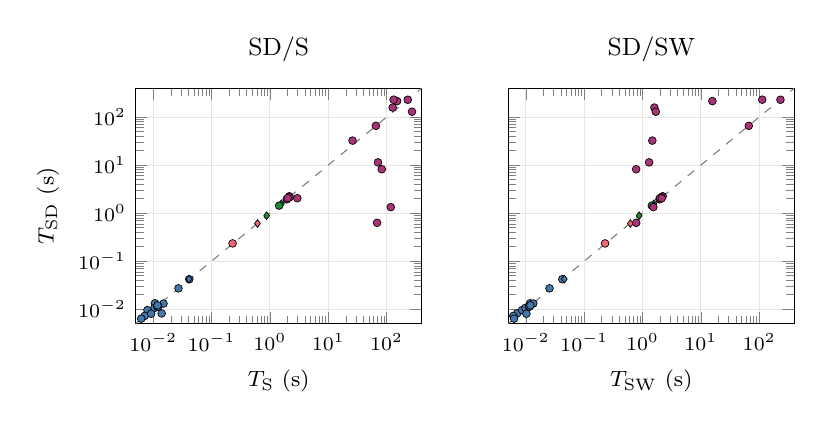
\begin{tikzpicture}
\begin{groupplot}[group style={group size=2 by 1,horizontal sep=11mm},
width=.43\textwidth,height=1.8in,xmode=log,ymode=log,
xmin=.005,xmax=400,ymin=.005,ymax=400,
xtick={.01,.1,1,10,100},ytick={.01,.1,1,10,100},
tick label style={font=\scriptsize},label style={font=\footnotesize},
title style={font=\small},grid=major,grid style={gray!20}]
\nextgroupplot[title={SD/S},xlabel={$T_{\mathrm{S}}$ (s)},ylabel={$T_{\mathrm{SD}}$ (s)}]
\addplot[gray,dashed,no marks] coordinates {(.005,.005) (400,400)};
\addplot[only marks,color=sizeblue,mark=*,mark size=1.4pt,mark options={draw=black,line width=.25pt}] coordinates {(0.0106881661,0.0132695418) (0.0139527917,0.00815941673) (0.00796033395,0.00958262524) (0.0150082912,0.0131057501) (0.0414693751,0.0420325422) (0.0105420412,0.0106582087) (0.00714958273,0.00724733295) (0.0117849591,0.0112175001) (0.0122545422,0.0113347918) (0.0118623753,0.0120392079) (0.00622904208,0.00635395804) (0.00919191632,0.00804429082) (0.0271031251,0.0272008749)};
\addplot[only marks,color=sizeblue,mark=diamond*,mark size=1.4pt,mark options={draw=black,line width=.25pt}] coordinates {(0.0410358752,0.0424029171) (1.57372021,1.57042554)};
\addplot[only marks,color=sizerose,mark=*,mark size=1.4pt,mark options={draw=black,line width=.25pt}] coordinates {(0.22921075,0.234206)};
\addplot[only marks,color=sizerose,mark=diamond*,mark size=1.4pt,mark options={draw=black,line width=.25pt}] coordinates {(0.613217042,0.608268083)};
\addplot[only marks,color=sizegreen,mark=*,mark size=1.4pt,mark options={draw=black,line width=.25pt}] coordinates {(1.44331437,1.43515742)};
\addplot[only marks,color=sizegreen,mark=diamond*,mark size=1.4pt,mark options={draw=black,line width=.25pt}] coordinates {(0.881013083,0.884120708)};
\addplot[only marks,color=sizepurple,mark=*,mark size=1.4pt,mark options={draw=black,line width=.25pt}] coordinates {(71.2466432,11.4136102) (82.8102985,8.21716367) (68.8015707,0.628461125) (151.570499,215.566638) (132.188374,230.463301) (2.13657354,2.13660808) (2.15772262,2.24763725) (2.17230025,2.13016629) (1.94581008,1.94049775) (2.01657846,2.05571879) (2.95261371,2.04632213) (127.547126,157.96961) (273.109595,129.327515) (118.231847,1.33494983) (231.004048,229.555527) (65.6820586,65.7308368) (26.1139253,32.3812967)};
\nextgroupplot[title={SD/SW},xlabel={$T_{\mathrm{SW}}$ (s)},yticklabels=\empty]
\addplot[gray,dashed,no marks] coordinates {(.005,.005) (400,400)};
\addplot[only marks,color=sizeblue,mark=*,mark size=1.4pt,mark options={draw=black,line width=.25pt}] coordinates {(0.0117819998,0.0132695418) (0.00709987525,0.00815941673) (0.00864183391,0.00958262524) (0.0134127089,0.0131057501) (0.0421956251,0.0420325422) (0.00982512487,0.0106582087) (0.00610820763,0.00724733295) (0.0112966672,0.0112175001) (0.0115406248,0.0113347918) (0.0119767906,0.0120392079) (0.0062699588,0.00635395804) (0.0102166254,0.00804429082) (0.0254336251,0.0272008749)};
\addplot[only marks,color=sizeblue,mark=diamond*,mark size=1.4pt,mark options={draw=black,line width=.25pt}] coordinates {(0.0456780419,0.0424029171) (1.57246708,1.57042554)};
\addplot[only marks,color=sizerose,mark=*,mark size=1.4pt,mark options={draw=black,line width=.25pt}] coordinates {(0.228360167,0.234206)};
\addplot[only marks,color=sizerose,mark=diamond*,mark size=1.4pt,mark options={draw=black,line width=.25pt}] coordinates {(0.618717042,0.608268083)};
\addplot[only marks,color=sizegreen,mark=*,mark size=1.4pt,mark options={draw=black,line width=.25pt}] coordinates {(1.44520921,1.43515742)};
\addplot[only marks,color=sizegreen,mark=diamond*,mark size=1.4pt,mark options={draw=black,line width=.25pt}] coordinates {(0.875552875,0.884120708)};
\addplot[only marks,color=sizepurple,mark=*,mark size=1.4pt,mark options={draw=black,line width=.25pt}] coordinates {(1.29770317,11.4136102) (0.778772125,8.21716367) (0.779829541,0.628461125) (15.7712266,215.566638) (112.791837,230.463301) (2.13614567,2.13660808) (2.218219,2.24763725) (2.12159946,2.13016629) (1.95401058,1.94049775) (1.99214796,2.05571879) (2.13044433,2.04632213) (1.59795042,157.96961) (1.69057658,129.327515) (1.53590675,1.33494983) (231.743763,229.555527) (66.3215101,65.7308368) (1.47419821,32.3812967)};
\end{groupplot}
\end{tikzpicture}
\caption{Audited complete-cost distribution at the fixed verified metric-SDP width target. Each panel shows all 36 jointly verified pairs among 43 planned cases; Table~\ref{tab:metric-main} retains other outcomes. The dashed line is equal cost, so points above it favor the reference. Blue, rose, green, and purple mark original sizes 1--32, 33--64, 65--128, and 129--300; diamonds mark development cases. Both axes use seconds on a log scale.}
\label{fig:metric-cost}
\end{figure*}

Figure~\ref{fig:metric-cost} displays the target-qualified pairs without
imputing a cost to a wall-limited case. The D stage removes additional vertices after S in 12 of 43 cases and none
in 31. Some controlled cases benefit against S: the best jointly verified
SD/S ratio is 0.009134. Yet SW's final quotient is no larger than SD's in
all 43 cases and strictly smaller in seven. Relative to SW, SD has no
additional verified completion, no ratio below 0.5 among the 36 jointly
verified cases, and seven ratios above 2; the largest is 98.857642. In that
case SD uses 158 complete compute seconds versus 1.598 for SW and has 182
quotient vertices versus SW's eight. The full ratio ranges are
0.009134--1.743446 for SD/S and 0.787373--98.857642 for SD/SW.
These finite, correlated controlled/development cases do not support an
IID confidence interval, broad solver claim, or a robust complete-cost
advantage over the strongest implemented reference. They leave the exact
contraction guarantee intact while failing to establish the planned
application-level utility endpoint.

\subsection{Correctness and non-dominance}
An independent exact-arithmetic audit checks all 729 signed four-vertex graphs
with pair weights in $\{-1,0,1\}$ and all 1,023 nonempty unweighted five-vertex
graphs, together with 120 weighted looped cases. It checks expected-copy
inequalities, fused optimal representatives, strict all-optima statements,
overlap composition, sparse formulas, and quotient preservation by enumerating
partitions. There are no assertion failures. These finite checks complement
the proofs and do not estimate large-graph coverage.

Degree weighting and uniform weighting are incomparable. One loopless
five-vertex example at $\gamma=1/8$ has a positive uniform certificate for a
two-vertex block while its exact degree-weighted pair margin is negative.
We retain it as a negative mechanism control. Likewise, two matched cliques
are already reducible by published collective rules; they test threshold
behavior rather than separation from prior preprocessing.

Appendix~\ref{app:comparison} gives small degree-specific and collective
examples, together with their recursive and oracle counterchecks.
Proposition~\ref{prop:guarded} combines both mechanisms in a connected family
at $\gamma=S/10^6$. Every Paley(29) block has a strict actual-median degree
certificate, while every original uniform candidate and every original
almost-clique subset fails, including the exhaustive polynomial search of
Schulz et al.~\cite{schulz2022cut}. Full similar-neighborhood pairs,
all repulsive cuts and all objective-faithful subgraph fusion conditions
also fail. The quantified proof covers unrestricted original searches.
Its growing resolution, ramp loops and surviving isolation-and-uniform
composition delimit the result; it is an analytic criterion comparison
separate from the frozen performance measurements.

\subsection{Public coverage and downstream utility}
Appendix Figure~\ref{fig:v2-coverage} reports the complete sequential comparison.
Median removed fractions over three discovery seeds range from 1.69\% to 35.12\%
for D, 0.10\% to 44.41\% for R, and 1.79\% to 49.54\% for RD.
The degree stage adds removals after its own fresh recursive prefix in 44 of
54 cases, with positive median additions in 14 of 18 graph--resolution settings.
The largest median addition is 1,587 vertices; the largest individual addition
is 1,618. Four settings have zero median additions, including both lower
resolutions of Gnutella. These are executed sequential reductions, rather than
a union of original-graph weak certificates. Table~\ref{tab:v2-coverage} and
Figure~\ref{fig:v2-rd-additional} retain every setting and its observed seed range.



Table~\ref{tab:v2-main} reports all five comparisons for the complete nine-call
workload; Table~\ref{tab:v2-prefixes} retains every correlated prefix.
For each setting, speedup is the median constructed standalone $T_B/T_A$
over the three fixed discovery seeds. Every D/U, R/U and RD/U setting has a
median below one at every prefix. At nine calls, these ranges are respectively
0.555--0.753, 0.378--0.751 and 0.322--0.636. Thus none of the measured
preprocessed Louvain workloads recovers its full cost against U.
Adding D after R also retains overhead in every setting: nine-call RD/R
medians range from 0.806 to 0.915. At that prefix, RD returns lower, equal and
higher exact original modularity than R in 26, 11 and 17 of 54 seed observations.
The 11 exact-quality matches have their own speedup range, 0.797--0.927;
none exceeds one. Prefixes reuse the same nine calls, so their observations
are not independent replications.

D is cheaper than R in 13, 12 and 11 of 18 setting medians at one, three and
nine calls, respectively. This does not establish a quality-matched general
advantage: at nine calls only two of 54 D/R observations have exactly equal
returned modularity, with speedups 0.954 and 1.526.
Safety preserves a global optimum, while a heuristic's returned objective
can change in either direction. The exact-Q comparisons therefore accompany
every cost comparison; Figures~\ref{fig:v2-utility} and~\ref{fig:v2-quality}
retain all 270 setting/comparison/prefix groups rather than selecting wins.

% BEGIN GENERATED V2 COMPARISON TABLE
\begin{table*}[t]
\caption{Complete nine-call V2 workloads, all five comparisons. Each row retains all 18 graph/resolution settings and 54 fixed-seed cases. Speedups are standalone $T_B/T_A$: the range spans setting medians, and $>1$ counts medians above one. Q counts are exact worse/equal/better outcomes for A versus B. Matched ranges retain every equal-Q seed and their own $n$. Table~\ref{tab:v2-prefixes} retains all three prefixes.}\label{tab:v2-main}
\centering\small
\begin{tabular}{lcrrrrr}\toprule
Pair & $k$ & Speedup range & $>1$/18 & Q worse/equal/better & Matches/54 & Matched range ($n$)\\\midrule
D/U & 9 & 0.55--0.75 & 0/18 & 31/3/20 & 3/54 & 0.59--0.62 (3)\\
R/U & 9 & 0.38--0.75 & 0/18 & 25/2/27 & 2/54 & 0.40--0.63 (2)\\
RD/U & 9 & 0.32--0.64 & 0/18 & 32/2/20 & 2/54 & 0.37--0.56 (2)\\
D/R & 9 & 0.93--1.54 & 11/18 & 34/2/18 & 2/54 & 0.95--1.53 (2)\\
RD/R & 9 & 0.81--0.92 & 0/18 & 26/11/17 & 11/54 & 0.80--0.93 (11)\\
\bottomrule\end{tabular}
\end{table*}
% END GENERATED V2 COMPARISON TABLE

The separate V1 study also retains complete-cost overhead; Appendix~\ref{app:additional-discrete-results} gives its unpooled summary and Appendix~\ref{app:v1-tables} all original observations.

The full native-solver study has 73 predeclared eligible pairs: 61 controlled
and 12 development pairs. Both native arms finish in 32 pairs, with exactly
equal lifted original modularity; one additional pair has an analytic one-node
quotient and is reported separately. The remaining 40 pairs retain timeouts,
domain exclusions or the recorded two-arm assertion. Across the 32 completed
native-only pairs, median runner speedup is 1.194, but median complete matched
pipeline speedup is 0.916; its observed range is 0.467--7.417. These ratios
condition on completion and do not characterize excluded pairs. Exact lifted
feasibility is independently checked; native search optimality relies on the
pinned solver rather than independent exhaustive verification.

\subsection{Mechanism and assembly scaling}
Appendix~\ref{app:additional-discrete-results} reports isolated assembly measurements
at block sizes 16 and 32, retaining exact-checker costs and a separately labeled
uncertified dense diagnostic. Median-checker time is 1.48--1.65 ms at $k=16$
and 6.02--6.31 ms at $k=32$, while traced peaks are 0.063 MiB and
0.209--0.240 MiB. The dense diagnostic reaches 4.70 and 8.37 MiB,
respectively; it performs no exact certification and can be faster on smaller
inputs. These finite measurements isolate representation cost. The current
CSR slice still allocates an $O(n)$ index workspace.

Controlled supplied-block results appear in Table~\ref{tab:mechanism-details}.
For the nine degree-heterogeneous reference blocks at $\gamma=1$, the median
and full-pair conditions accept all nine while uniform copying accepts three.
The reverse five-vertex example remains an explicit non-dominance control.
On common-hub blocks at $\gamma=1$, the median center accepts both supplied
blocks while the zero center accepts one. The exploratory incompatible private-leaf
blocks are rejected by every exact copy variant. Over all 17,405 recorded
AUTO-versus-forced-exact block comparisons, forced exact checking accepts 64
additional blocks and there are no AUTO-only accepts. Screening therefore
loses coverage in this study; exact certification remains the acceptance gate.
Unavailable uniform comparisons and numerical isolation matches retain
their separate statuses and never count as certified rejections or accepts.

\subsection{Exploratory global-optimum audit}
A separately reviewed post-freeze audit applies the same exact proof policy to
the original, degree-certificate, and recursive-reference graphs: nonpositive
off-diagonal modularity weights certify the singleton optimum; otherwise,
enumerate every partition only when the represented graph has at most ten
vertices. Quotient proofs establish an original optimum only with their saved
safety dependencies. Degree certificates are rechecked exactly; recursive
dependencies replay the frozen reference implementation and do not constitute
an independent reimplementation of its criteria. This audit retains 193
resolution tuples and 579 arm rows, including unresolved and unavailable rows.

\begin{table}[t]
\caption{Tuples with an established original optimum under the identical capped
audit policy. This is exploratory proof coverage, with no timing endpoint.}
\label{tab:global-audit}
\centering
\begin{tabular}{lrrrr}\toprule
Input group & Tuples & Original & Degree & Recursive\\\midrule
Controlled &127&15&58&27\\
Public &54&0&0&0\\
Development &12&0&0&0\\\bottomrule
\end{tabular}
\end{table}

Table~\ref{tab:global-audit} shows 59 distinct controlled tuples established
in at least one arm. The degree arm establishes 32 tuples unresolved by both
other arms: 22 noisy planted, eight matched-clique, and two common-hub tuples.
Conversely, one tuple is established only by the recursive arm. Overall, 100
arm rows are established, 461 remain unresolved, and 18 are unavailable.
All public and development tuples remain unresolved under this limited policy.
Thus additional safe reductions can expose simple exact proofs on the controlled
grid, without establishing public-graph global optima or general solver dominance.

\section{Conclusion}
Degree-weighted anchor copying cancels modularity's exterior null model and
produces a collective contraction test from sparse normalized adjacency
profiles. Exact verification, compatible overlap and a quantitative loss
bound accompany the certificate. On the declared public grid, it adds safe
reductions after recursive criteria in 44 of 54 cases, but neither standalone
nor sequential preparation amortizes in the measured Louvain workloads.
Controlled quotients expose additional exact proofs under a fixed capped
policy; public global optima remain unresolved. The audited metric-SDP
comparison also finds no robust complete-cost advantage over the stronger
full-pair control. The contribution is a complementary sufficient condition
whose correctness, coverage and solver utility have separate evidence.

\begin{thebibliography}{99}
\bibitem{louf2024expansion}Baptiste Louf, Colin McDiarmid, and Fiona Skerman. 2024. Modularity and Graph Expansion. \emph{15th Innovations in Theoretical Computer Science Conference (ITCS 2024)} 287: 78:1--78:21. \url{https://doi.org/10.4230/LIPIcs.ITCS.2024.78}

\bibitem{lorena2019clique}Luiz Henrique Nogueira Lorena, Marcos Gon{\c c}alves Quiles, and Luiz Antonio Nogueira Lorena. 2019. Improving the Performance of an Integer Linear Programming Community Detection Algorithm Through Clique Filtering. \emph{Computational Science and Its Applications -- ICCSA 2019} 11619: 757--769. \url{https://doi.org/10.1007/978-3-030-24289-3_56}

\bibitem{newman2006modularity}M. E. J. Newman. 2006. Modularity and community structure in networks. \emph{Proceedings of the National Academy of Sciences} 103(23): 8577--8582. \url{https://doi.org/10.1073/pnas.0601602103}

\bibitem{reichardt2006statistical}J{\"o}rg Reichardt, and Stefan Bornholdt. 2006. Statistical mechanics of community detection. \emph{Physical Review E} 74(1): 016110. \url{https://doi.org/10.1103/PhysRevE.74.016110}

\bibitem{arenas2007size}A. Arenas, J. Duch, A. Fern{\'a}ndez, and S. G{\'o}mez. 2007. Size reduction of complex networks preserving modularity. \emph{New Journal of Physics} 9(6): 176. \url{https://doi.org/10.1088/1367-2630/9/6/176}

\bibitem{lange2018partial}Jan-Hendrik Lange, Andreas Karrenbauer, and Bjoern Andres. 2018. Partial Optimality and Fast Lower Bounds for Weighted Correlation Clustering. \emph{Proceedings of the 35th International Conference on Machine Learning} 80: 2892--2901. \url{https://proceedings.mlr.press/v80/lange18a.html}

\bibitem{lange2019combinatorial}Jan-Hendrik Lange, Bjoern Andres, and Paul Swoboda. 2019. Combinatorial Persistency Criteria for Multicut and Max-Cut. \emph{IEEE/CVF Conference on Computer Vision and Pattern Recognition}. \url{https://doi.org/10.1109/CVPR.2019.00625}

\bibitem{bocker2011exact}Sebastian B{\"o}cker, Sebastian Briesemeister, and Gunnar W. Klau. 2011. Exact Algorithms for Cluster Editing: Evaluation and Experiments. \emph{Algorithmica} 60(2): 316--334. \url{https://doi.org/10.1007/s00453-009-9339-7}

\bibitem{schulz2022cut}Hjalmar Schulz, Andr{\'e} Nichterlein, Rolf Niedermeier, and Christopher Weyand. 2022. Applying a Cut-Based Data Reduction Rule for Weighted Cluster Editing in Polynomial Time. \emph{17th International Symposium on Parameterized and Exact Computation (IPEC 2022)} 249: 25:1--25:14. \url{https://doi.org/10.4230/LIPIcs.IPEC.2022.25}

\bibitem{blasius2022branch}Thomas Bl{\"a}sius, Philipp Fischbeck, Lars Gottesb{\"u}ren, Michael Hamann, Tobias Heuer, Jonas Spinner, Christopher Weyand, and Marcus Wilhelm. 2022. A Branch-And-Bound Algorithm for Cluster Editing. \emph{20th International Symposium on Experimental Algorithms} 233: 13:1--13:19. \url{https://doi.org/10.4230/LIPIcs.SEA.2022.13}

\bibitem{stein2025partial}David Stein, Bjoern Andres, and Silvia Di Gregorio. 2025. Partial Optimality in Cubic Correlation Clustering for General Graphs. arXiv:2510.20431. Preprint, version 1. \url{https://doi.org/10.48550/arXiv.2510.20431}

\bibitem{nowozin2009solution}Sebastian Nowozin, and Stefanie Jegelka. 2009. Solution Stability in Linear Programming Relaxations: Graph Partitioning and Unsupervised Learning. \emph{Proceedings of the 26th International Conference on Machine Learning}. \url{https://icml.cc/2009/papers/95.pdf}

\bibitem{veldt2017correlation}Nate Veldt, Anthony Wirth, and David F. Gleich. 2017. Correlation Clustering with Low-Rank Matrices. \emph{Proceedings of the 26th International Conference on World Wide Web} 1025--1034. \url{https://doi.org/10.1145/3038912.3052586}

\bibitem{floros2023fiedler}Dimitris Floros, Nikos Pitsianis, and Xiaobai Sun. 2023. The Fiedler connection to the parametrized modularity optimization for community detection. arXiv:2310.14359. Preprint, version 1. \url{https://doi.org/10.48550/arXiv.2310.14359}

\bibitem{blondel2008fast}Vincent D. Blondel, Jean-Loup Guillaume, Renaud Lambiotte, and Etienne Lefebvre. 2008. Fast unfolding of communities in large networks. \emph{Journal of Statistical Mechanics: Theory and Experiment} (10): P10008. \url{https://doi.org/10.1088/1742-5468/2008/10/P10008}

\bibitem{leskovec2014snap}Jure Leskovec, and Andrej Krevl. 2014. {SNAP Datasets}: {Stanford} Large Network Dataset Collection. \url{https://snap.stanford.edu/data/}

\bibitem{leskovec2007graph}Jure Leskovec, Jon Kleinberg, and Christos Faloutsos. 2007. Graph Evolution: Densification and Shrinking Diameters. \emph{ACM Transactions on Knowledge Discovery from Data} 1(1): 2. \url{https://doi.org/10.1145/1217299.1217301}

\bibitem{yin2017local}Hao Yin, Austin R. Benson, Jure Leskovec, and David F. Gleich. 2017. Local Higher-Order Graph Clustering. \emph{Proceedings of the 23rd ACM SIGKDD International Conference on Knowledge Discovery and Data Mining} 555--564. \url{https://doi.org/10.1145/3097983.3098069}

\bibitem{mcauley2012learning}Julian McAuley, and Jure Leskovec. 2012. Learning to Discover Social Circles in Ego Networks. \emph{Advances in Neural Information Processing Systems} 25. \url{https://papers.nips.cc/paper_files/paper/2012/hash/7a614fd06c325499f1680b9896beedeb-Abstract.html}

\bibitem{ripeanu2002mapping}Matei Ripeanu, Ian Foster, and Adriana Iamnitchi. 2002. Mapping the {Gnutella} Network: Properties of Large-Scale Peer-to-Peer Systems and Implications for System Design. arXiv:cs/0209028. Technical-report version. \url{https://arxiv.org/abs/cs/0209028}

\bibitem{jia2020certified}Jinyuan Jia, Binghui Wang, Xiaoyu Cao, and Neil Zhenqiang Gong. 2020. Certified Robustness of Community Detection against Adversarial Structural Perturbation via Randomized Smoothing. \emph{Proceedings of The Web Conference 2020}. \url{https://doi.org/10.1145/3366423.3380029}

\bibitem{gokavarapu2026finite}Chandrasekhar Gokavarapu, Sekhar Babu Gosala, Rajeev Muthu, Vamsi Pasalapudi, and Tarakarama Kapakayala. 2026. Finite-sample certification and operating envelopes for spectral clustering and graph centrality. arXiv:2602.10566. Preprint, version 2, 29 July 2026. \url{https://doi.org/10.48550/arXiv.2602.10566}

\bibitem{wang2026netptr}Wanjie Wang, and Tao Shen. 2026. {NetPTR}: Optimal Differentially Private Spectral Community Detection on Sparse Networks. arXiv:2606.26145. Preprint, version 1. \url{https://doi.org/10.48550/arXiv.2606.26145}

\bibitem{ling2020certifying}Shuyang Ling, and Thomas Strohmer. 2020. Certifying Global Optimality of Graph Cuts via Semidefinite Relaxation: A Performance Guarantee for Spectral Clustering. \emph{Foundations of Computational Mathematics} 20: 367--421. \url{https://doi.org/10.1007/s10208-019-09421-3}

\bibitem{chen2018convexified}Yudong Chen, Xiaodong Li, and Jiaming Xu. 2018. Convexified Modularity Maximization for Degree-corrected Stochastic Block Models. \emph{The Annals of Statistics} 46(4): 1573--1602. \url{https://doi.org/10.1214/17-AOS1595}

\bibitem{hildebrand2008convex}Roland Hildebrand. 2008. Identification of community structure in networks with convex optimization. arXiv:0806.1896. Preprint, version 2, 12 June 2008. \url{https://arxiv.org/abs/0806.1896v2}

\bibitem{mathieu2010correlation}Claire Mathieu and Warren Schudy. 2010. Correlation Clustering with Noisy Input. \emph{Proceedings of the Twenty-First Annual ACM-SIAM Symposium on Discrete Algorithms}, 712--728. \url{https://doi.org/10.1137/1.9781611973075.58}

\bibitem{wang2020community}Po-Wei Wang and J. Zico Kolter. 2020. Community detection using fast low-cardinality semidefinite programming. \emph{Advances in Neural Information Processing Systems} 33. \url{https://proceedings.neurips.cc/paper/2020/hash/229aeb9e2ae66f2fac1149e5240b2fdd-Abstract.html}

\bibitem{jansson2008rigorous}Christian Jansson, Denis Chaykin, and Christian Keil. 2008. Rigorous error bounds for the optimal value in semidefinite programming. \emph{SIAM Journal on Numerical Analysis} 46(1). \url{https://doi.org/10.1137/050622870}

\bibitem{shekhovtsov2014persistency}Alexander Shekhovtsov. 2014. Maximum Persistency in Energy Minimization. arXiv:1404.3653. Research report, version 2, 16 June 2014. \url{https://arxiv.org/abs/1404.3653v2}
\bibitem{permenter2020jordan}Frank Permenter and Pablo A. Parrilo. 2020. Dimension reduction for semidefinite programs via Jordan algebras. \emph{Mathematical Programming} 181: 51--84. \url{https://doi.org/10.1007/s10107-019-01372-5}

\bibitem{diamond2016cvxpy}Steven Diamond and Stephen Boyd. 2016. CVXPY: A Python-Embedded Modeling Language for Convex Optimization. \emph{Journal of Machine Learning Research} 17(83): 1--5. \url{https://www.jmlr.org/papers/v17/15-408.html}

\bibitem{odonoghue2016scs}Brendan O'Donoghue, Eric Chu, Neal Parikh, and Stephen Boyd. 2016. Conic Optimization via Operator Splitting and Homogeneous Self-Dual Embedding. \emph{Journal of Optimization Theory and Applications} 169(3): 1042--1068. \url{https://doi.org/10.1007/s10957-016-0892-3}

\bibitem{avis1991cutcone}David Avis and Michel Deza. 1991. The cut cone, $L^1$ embeddability, complexity, and multicommodity flows. \emph{Networks} 21(6): 595--617. \url{https://doi.org/10.1002/net.3230210602}

\bibitem{kyng2015connection}Rasmus Kyng, Yin Tat Lee, Richard Peng, Sushant Sachdeva, and Daniel A. Spielman. 2015. Sparsified Cholesky and Multigrid Solvers for Connection Laplacians. arXiv:1512.01892. Preprint, version 1. \url{https://arxiv.org/abs/1512.01892v1}

\end{thebibliography}

\appendix
\section{Proof Details}\label{app:proofs}
\subsection{The exterior expansion}
For fixed $w\notin K$, the initial contribution is
$\sum_u B_{uw}x_u^w$. After copying to anchor $r$, it is
$\sum_u B_{uw}x_r^w$. Hence
\[
 -\E_r\Delta F_w=\sum_u B_{uw}x_u^w-
 V^{-1}\sum_{u,r}d_r B_{uw}x_r^w.
\]
Multiplying the first term by $V/V$, pairing ordered terms for $u\ne r$, and
renaming $r$ as $v$ gives
$V^{-1}\sum_{u<v}(d_vB_{uw}-d_uB_{vw})(x_u^w-x_v^w)$.
The diagonal ordered terms cancel. Summing over exterior vertices proves
Eq.~\eqref{eq:expansion}. The degree-product part of $B$ cancels inside each
bracket, proving Eq.~\eqref{eq:pairpenalty}. For a separated pair,
$|x_u^w-x_v^w|\leq 1$; for an unseparated pair it is zero.

\subsection{The center's quadratic form}\label{app:center-quadratic}
Define $h_{uv}=(d_ud_v/V)(\delta_u+\delta_v)$. Expanding the pair sum for any
$x\in\R^k$ gives
\begin{align*}
 x^\top L(h)x
 &=\sum_u d_u(\delta_u+\bar\delta)x_u^2\\
 &\quad-\frac 2V\left(\sum_ud_u\delta_u x_u\right)
                    \left(\sum_ud_u x_u\right).
\end{align*}
The second term vanishes on $d_K^\perp$. Also
\[
 L(B_K)=L(A_K)-\frac\gamma S(VW-d_Kd_K^\top).
\]
Since $P_{uv}^{\rm ext}\leq h_{uv}$, the relaxed contrast
$L(B_K-h)$ is no greater than the exact contrast in positive semidefinite
order. On $d_K^\perp$ it is precisely the quadratic form in
Eq.~\eqref{eq:rational}. Positivity there is equivalent to positivity on
$\1^\perp$, because both Laplacians kill $\1$ and $d_K^\top\1=V>0$.
The partition-indicator decomposition then proves Theorem~\ref{thm:fusion}.

\subsection{Quantitative loss}
For each induced group $K_j$, translate its indicator to
$y_j=\1_{K_j}-(v_j/V)\1$. Then $d_K^\top y_j=0$ and
$y_j^\top W y_j=v_j-v_j^2/V$. Applying the lower Rayleigh bound to every
indicator gives Eq.~\eqref{eq:quantgain}. Splitting a positive group into
individual vertices decreases $\sum_jv_j^2$, so the dispersion is at most
$V-\sum_ud_u^2/V$. At least one anchor attains the expected lower bound.
Starting at a global optimum therefore loses at most half of
$\max(0,-\mu)$ times this dispersion in $F$. Multiplying by $2/S$ proves
Eq.~\eqref{eq:regret}. For disjoint blocks, copying one never splits an
already fused block; summing their bounds is valid.

\subsection{Center transport through coarsening}\label{app:transport}
Retain the assumptions of Theorem~\ref{thm:fusion}. Partition the original
vertices into nonempty groups, each wholly inside $K$ or wholly outside it,
and use the exact degree-preserving quotient, including its diagonal.
Let $C$ indicate the groups inside $K$, which form $K'$.
For an exterior group $b$, transport the center as
$c'_b=\sum_{w\in b}c_w$.

\begin{lemma}[Center transport]\label{lem:transport}
If $|K'|\ge2$, the restricted minimum computed with the transported center
satisfies $\lambda'\ge\lambda$. The resolution threshold is unchanged, so
weak and strict center certificates remain valid. If $|K'|=1$, fusion is
already represented and no singleton test is needed.
\end{lemma}
\begin{proof}
For an internal group $a$, its normalized exterior row is a degree-weighted
mixture of original rows followed by exterior-coordinate summation. Triangle
inequality gives
\[
 d'_a\delta'_a\le\sum_{u\in a}d_u\delta_u,
 \qquad \bar\delta'\le\bar\delta.
\]
Exact quotienting gives $L(A'_{K'})=C^\top L(A_K)C$,
$W'=C^\top WC$, and $S'=S$, $V'=V$.
For $y\ne0$ with $(d'_{K'})^\top y=0$, set $x=Cy$.
This injective pullback has $d_K^\top x=0$ and identical weighted norm.
Because $x_u=y_a$ within group $a$, the deviation inequalities imply
\begin{align*}
 &y^\top[L(A'_{K'})-\diag\{d'_a(\delta'_a+\bar\delta')\}]y\\
 &\quad\ge x^\top[L(A_K)-\diag\{d_u(\delta_u+\bar\delta)\}]x
 \ge\lambda y^\top W'y.
\end{align*}
Taking the quotient restricted minimum proves the claim.
\end{proof}
For rational coefficients this is also an exact proof transport: the quotient
threshold form is $C^\top H_\theta C$ plus a nonnegative diagonal correction,
where $H_\theta=L(A_K)-\diag\{d_u(\delta_u+\bar\delta+\theta)\}$ and
$\theta=\gamma V/S$.
The algebra does not require a safe coarsening; lifting a quotient optimum to
an original optimum separately requires that coarsening's safety guarantee.
Quotient strictness following merely weak safety does not itself imply an
all-original-optima conclusion.

The center premise matters. Take nine core vertices, every distinct internal
edge of weight $t=1/16$. Six core loops have weight $1/2$; the other three
loops have weight $7/16$, and each of those vertices has one edge of weight $t$
to the same exterior vertex, which has no loop. Every core full degree is one,
$V=9$ and $S=147/16$. The exterior profiles are six zeros and three $t$'s,
so the original median is zero, $\bar\delta=t/3$, and
$L(A_K)=t(9I-J)$. A contrast between two nonzero-profile vertices attains
$\lambda=23t/3=23/48$.
Contract the six zero-profile vertices into two triples, leaving the others
separate. Quotient core degrees are $(3,3,1,1,1)$; on the weighted contrast
space its internal normalized Laplacian still equals $9tI$.
The transported center remains zero and attains the same $\lambda'$.
Its recomputed unweighted median is instead $t$, with deviations
$(t,t,0,0,0)$ and mean $2t/3$. A contrast between the two triple groups
attains $\lambda'_{\rm median}=22t/3=11/24$.
At $\gamma=245/512$, the threshold is $15/32$, so the original and transported
margins are $1/96$, while the new-median margin is $-1/96$.
The original strict certificate fuses the entire core in every optimum, making
these triple contractions safe. Thus even safe coarsening need not preserve
acceptance under a recomputed median. This is an analytic example, not a
measured checker run. The frozen sequential implementation rechecks its actual
current quotient and median; it does not implement center transport or claim
automatic acceptance containment.

\subsection{Attainment of the threshold and loss bound}\label{app:sharpness}
Take the entire loopless unit-weight complete graph on $k\ge2$ vertices as $K$.
Then $d_u=k-1$, $V=S=k(k-1)$, and the empty exterior gives
$\delta=\bar\delta=0$. On $\1^\perp$, the normalized internal Laplacian
is $k/(k-1)$ times the identity, so $\mu=k/(k-1)-\gamma$.
Every off-diagonal affinity equals
$b=1-\gamma(k-1)/k=\mu(k-1)/k$.
If $\mu>0$, the unique optimum fuses all vertices; at $\mu=0$, every
partition is optimal; if $\mu<0$, the unique optimum consists of singletons.
Thus weak fusion at equality and the strict all-optima statement have the
sharp distinction in Theorem~\ref{thm:fusion}.
In the negative-margin case, singleton and fused modularities are
$-\gamma/k$ and $1-\gamma$, respectively. Their gap is
\[
 \gamma(1-1/k)-1=-\mu(1-1/k),
\]
exactly Eq.~\eqref{eq:regret}, since
$\sum_ud_u^2/V=k-1$.
For any partition with block sizes $h_j$, its expected copy gain is
$b(k^2-\sum_jh_j^2)/2$, also exactly Eq.~\eqref{eq:quantgain}.
This elementary attainment example concerns the bounds' worst case, not
practical completeness of the sufficient certificate.

\subsection{Overlap and the zero-degree exception}
Within a connected component of the block-intersection graph, choose a traversal
in which each new block intersects the previous union. Apply the first
certificate to an optimum. At every subsequent step, select an anchor in the
intersection. It has positive degree and hence positive probability. The
optimal-anchor lemma preserves the objective, and all vertices in the previous
union remain in its community. Disjoint intersection components can be
processed successively.

The positive-degree requirement is substantive. Take unit edges $(1,4)$ and
$(2,3)$ and isolated vertex 0, at resolution 1. Each edge plus vertex 0 can be
fused in some optimum, but the optimum separates the two edges. Requiring both
blocks fused forces all positive-degree vertices together. An anchor at vertex 0
has zero probability, so the overlap proof cannot use that intersection.

\section{Criterion Comparisons}\label{app:comparison}
\subsection{The pair specialization}
For a separated attractive pair, write $a(P)$ and $b(P)$ for the exterior
losses of its two directional copies, excluding the mutual gain $B_{uv}$.
For any positive anchor probabilities, the smaller loss satisfies
\[
 \min\{a(P),b(P)\}\leq\pi_v a(P)+\pi_u b(P)
 \leq\sum_{w\notin\{u,v\}}|\pi_vB_{uw}-\pi_uB_{vw}|.
\]
The last inequality bounds the expected exterior loss. Maximizing the left
side over exterior assignments gives the exact similar-neighborhood threshold
of B\"ocker et al.~\cite{bocker2011exact}. Thus acceptance by the degree-copy
pair penalty implies acceptance by that rule. A center relaxation can only
increase the penalty. Zero mutual affinity with zero penalty is covered by
proportional weighted twins~\cite{blasius2022branch}. We do not attribute a
new strongest pair rule to the proposed certificate.

\subsection{A degree-specific collective example}
The following rational construction is an algebraic comparison, obtained
during the post-freeze conceptual review; it is not a benchmark point.
Let $K=\{0,1,2,3\}$ have cycle weights
$A_{01}=8$ and $A_{12}=A_{23}=A_{30}=6$.
There are 20 independent exterior vertices, each adjacent to vertices 0,1
with weight 7 and to vertices 2,3 with weight 6. Divide these exterior vertices
into two classes of ten, and attach each class to its own new anchor by edges
of weight 200. All other entries, including loops, are zero. Use
$\gamma=2273/1750$. Then
\begin{align*}
 d_K&=(154,154,132,132),& d_E&=226,\\
 d_{\rm anchor}&=2000,& S&=9092,\\
 \gamma/S&=1/7000.
\end{align*}
The normalized exterior profiles equal $1/22$ on each exterior vertex and zero
on the anchors. Hence a median center gives $\delta=0$. The restricted internal
spectrum is $\{13/154,15/154,2/11\}$. To obtain it, divide the cycle weights
by two: its internal degrees are $(7,7,6,6)$, and the normalized adjacency has
bipartite singular values 1 and $1/14$. The original full degrees are 22 times
these degrees. Consequently
\[
 \lambda-\gamma V/S=13/154-143/1750=26/9625>0.
\]
The proposed test therefore forces all of $K$ together in every optimum.

For a high-degree and a low-degree core vertex, the uniform exterior row
contrast is
$D=20(507/1750)+2(44/7)=3214/175$.
The signed internal cut between $\{0,1\}$ and $\{2,3\}$ is $48/125$.
After uniform-copy penalties, its energy is
$48/125-D=-15734/875<0$, proving failure of the uniform PSD test.

For direct positive-closure comparison, retain every internal signed affinity
of an induced witness $H$, as in our reference implementation of
Lange's Appendix Theorem 4~\cite{lange2019combinatorial}.
Write $b_H=3549/1750$ and $b_L=1521/875$ for the core-to-exterior affinities.
Any witness containing an anchor has a negative cut separating its core
vertices: each high-degree vertex contributes at most
$20b_H-44=-602/175$, and each low-degree vertex at most
$20b_L-264/7=-516/175$. Its zero minimum-multicut premise fails.
If a witness contains exterior vertices but no anchor, its positive boundary
is at least $948/7$, while a singleton core cut in its positive closure costs
at most $13489/1750+20b_H=84469/1750<948/7$.
A witness containing only core vertices and a target pair has boundary at
least $40b_L=60840/875$, also larger than this cut bound.
Thus these direct full-induced witnesses cannot certify a core pair.
The comparison does not assert separation under a selected-edge convention
that discards internal objective interactions.
Isolating $C=K$ also fails the C-subinstance premise: adding one exterior vertex
gains $2b_H+2b_L=6591/875>0$.

\subsection{The recursive countercheck}
The same construction has a stronger prior reduction sequence.
An exterior class with its anchor has internal cut
$q[s-(10-q)c]>0$ when $q$ class vertices are separated, where
$s=948/7$ and $c=12769/1750$.
Its positive boundary is $10T$, where $T=6591/875$.
Every target-separating positive-closure cut costs at least
\begin{align*}
 &\min_{1\leq q\leq10}\{qs-q(10-q)c+\min(q,10-q)T\}\\
 &\qquad=135261/1750>10T=131820/1750.
\end{align*}
Hence prior positive-closure conditions strictly fuse each exterior class and
its anchor. After both fusions, core-to-class affinities are negative:
$-4151/175$ for high-degree vertices and $-3558/175$ for low-degree vertices.
The almost-clique condition on $K$ then has positive internal minimum cut
$5418/875$, negative internal mass $5082/875$, and zero positive exterior mass.
It certifies $K$ strictly by $336/875$.
The new condition therefore provides a direct local certificate in this
example, while a stronger recursive collective route recovers the same fusion.
This distinction must not be reported as superiority over complete prior
preprocessing or exact optimization.

\subsection{Collective fusion beyond the cheap starting fixed point}
\label{app:paley}
Let $P$ be the Paley graph on $\mathbb{F}_{29}$: two distinct residues are
adjacent when their difference is a nonzero square. It is undirected and
14-regular. The quadratic-character sum
$\sum_x\chi((x-a)(x-b))=-1$ for $a\ne b$ gives six common neighbors for
adjacent vertices and seven for nonadjacent vertices. To verify the sum,
an affine change reduces it to $\sum_x\chi(x^2-c)=-1$ for $c\ne0$.
The equation $y^2=x^2-c$ has 28 solutions, since
$(x-y)(x+y)=c$ and 2 is invertible. These counts give
\[
 A_P^2+A_P=7(I+J),\qquad
 \lambda_2(L_P)=(29-\sqrt{29})/2.
\]
The two nonconstant adjacency eigenvalues are
$(-1\pm\sqrt{29})/2$, each with multiplicity 14.

Connect two copies of $P$ by their corresponding-vertex perfect matching.
The resulting graph $G$ has 58 vertices, 435 edges, full degree 15 and
$S=870$. At $\gamma=1$, every positive pair affinity is
$\alpha=43/58$ and every negative one is $-\beta=-15/58$.
For a whole copy $K$, the median exterior center is zero and
$\delta_u=\bar\delta=1/15$: each exterior column has one matching incidence
and 28 zeros. Its block volume is $V=435$. Theorem~\ref{thm:fusion} has margin
\[
 \mu=\frac{\lambda_2(L_P)-2}{15}-\frac12
     =\frac{10-\sqrt{29}}{30}>0.
\]
Thus both copies fuse in every optimum. Their quotient has
\[
 A'=\begin{pmatrix}406&29\\29&406\end{pmatrix},\quad
 d'=(435,435),\quad B'_{12}=-377/2.
\]
Its separated partition has $Q=13/30$; joining gives zero. The two-copy
partition is consequently the unique original optimum, up to labels.
An independent rational projection of $L_P-(19/2)I$ onto $\1^\perp$
has 28 strictly positive exact elimination pivots. It verifies the same
definiteness without floating eigenvalues; the second copy follows by
isomorphism. This is a certificate-plus-quotient proof, not enumeration of
all 58-vertex partitions.

\paragraph{No original subset passes almost-clique.}
For an arbitrary subset $U$ of size $h\ge2$, let $e,m,b$ count its positive
internal edges, internal nonedges and positive boundary edges. Write
$\kappa$ for its positive weighted internal mincut, with $\kappa=0$ if
disconnected. B\"ocker Rule4~\cite{bocker2011exact} requires
$\kappa\ge\beta m+\alpha b$, while a singleton cut always gives
$\kappa\le\alpha\min(h-1,15)$.
For $2\le h\le15$, regularity gives
$b=15h-2e\ge h(16-h)>h-1$, so boundary mass alone defeats the condition.
The symmetric and antisymmetric modes of
$\left(\begin{smallmatrix}A_P&I\\I&A_P\end{smallmatrix}\right)$ give
$\lambda_2(L_G)=2$. For $16\le h\le31$, the centered indicator bound gives
$b\ge2h(58-h)/58\ge1344/58>15$, again exceeding the mincut bound.
For $32\le h\le58$, $e\le15h/2$ gives
$m\ge h(h-16)/2\ge256$, and
$\beta m\ge3840/58>645/58=15\alpha$.
These exhaustive ranges exclude even the weak condition on every original
subset, independently of the proposed bank.

\paragraph{No eligible original pair passes similar-neighborhood.}
Check the full max-min expression of B\"ocker Rule5~\cite{bocker2011exact},
rather than replacing it by a general half-contrast bound. A positive edge has
$t=6$ common positive neighbors inside a copy and $t=0$ across the matching.
Both exclusive-neighborhood offsets in the source rule are $a=14-t$.
On its remaining set $W$, the signed rows agree, so the two directional
terms are $a+z$ and $a-z$ for any two disjoint chosen subsets of $W$.
Their minimum is at most $a$, and the empty subsets attain $a$.
The exact right-hand side is therefore 8 or 14, both greater than
$B_{uv}=43/58$. Negative pairs are ineligible for this attractive rule.

\paragraph{The specified recursion and the oracle boundary.}
Singleton dominance has margin $-1189/58$ on every positive edge.
The single-edge positive-closure criterion~\cite{lange2019combinatorial}
has margin $(t-27)\alpha<0$. Every positive edge has an exclusive positive
neighbor, at which its two signed rows have opposite signs; no positive
proportional factor satisfies Twin Simple~\cite{blasius2022branch}.
Together with the all-subset almost-clique failure, these facts show that
the specified cheap pure-merge recursion has no first contraction.
Adding original Rule5 would not supply one. Arbitrary-subgraph criteria,
other cannot-link or bound-based reductions, and complete solving are outside
this exclusion.

Uniform copying also yields $L_P-(19/2)I$ on $\1^\perp$; equal degrees make
this example unable to distinguish the anchor distributions.
Moreover, the supplied-C isolation premise~\cite{blasius2022branch}
\emph{holds} for $C=K$. The C-subinstance retains all interactions incident
to $K$ and zeros only exterior-exterior interactions. Its same uniform-copy
certificate strictly fuses $K$. Each exterior vertex has total affinity
$\alpha-28\beta=-377/58<0$ to fused $K$; removing it incurs no
exterior-exterior loss. Isolating $K$ is therefore subinstance-optimal.
Scaling all signed costs by 58 gives equivalent integer costs 43 and $-15$,
consistent with the source's integer formulation. The example distinguishes
a cheap sufficient certificate from the named local merge rules, while
remaining covered by the more general isolation oracle.

\subsection{A joint original-instance separation}\label{app:guarded}
The following construction distinguishes degree-weighted collectivity from
unrestricted searches of several named initial predicates. All costs in this
subsection use the original $B=A-\beta dd^\top$ with $\beta=10^{-6}$.
The positive-support graph is connected.

For an integer $m\ge5000$, take two core Paley(29) copies $P_1,P_2$ with
weight 999 on Paley edges and their same-index matching. Each has a loop 999
at index 0 and an additional loop $39i$ at index $i=0,\ldots,28$.
For each $j\in\mathbb Z_m$, take remote copies $R_j^a,R_j^b$ with the same
weight 999 Paley edges and matching, and loops $39i$, without the extra
index 0 loop. Add weight 400 edges from $(R_j^b)_i$ to $(R_{j+1}^a)_i$.
A bridge $w_j$ connects to $(P_1)_0$ with weight $36/m$, to each other
$P_1$ vertex with weight $35/m$, and to $(R_j^a)_0$ with weight $600/m$.
Set $\gamma=\beta S$. Scaling the whole adjacency by $m$, while keeping
$\gamma$ fixed, gives an equivalent integer-weight instance.

The core volumes are $V_1=452414,V_2=451398$; remote volumes are
$V_R=461999$ for each $b$-half and $V_R+\epsilon$ for each $a$-half,
where $\epsilon=600/m$. Bridges have degree $1616/m$, and
\[
 n=58+59m,\qquad S=906028+923998m.
\]
Core degrees are $16020$ at $(P_1)_0$ and $15020+39i$ otherwise;
they are $15984$ at $(P_2)_0$ and $14985+39i$ otherwise.
Remote degrees are $15385+39i$, with extra $\epsilon$ at $(R_j^a)_0$.
Every nonbridge degree lies in $[15024,16477]$ and every off-diagonal
adjacency row sums to less than 15386.

\begin{proposition}\label{prop:guarded}
For every integer $m\ge5000$, all $2m+2$ Paley copies have strict
degree-profile certificates with their actual coordinate medians.
The unique optimal partition consists of $P_1$ with all bridges,
$P_2$ separately, and every remote Paley copy separately.
No nontrivial original subset passes the uniform-copy PSD condition or
almost-clique Rule 4. No original positive pair passes full Rule 5,
singleton dominance, single-edge positive closure or positive-factor twins;
original heavy Rules 1--3 also refuse. No original negative pair passes
Lange's repulsive-cut condition for any separating cut, and no target
passes its subgraph-fusion condition on an objective-faithful original
subgraph. A conditional isolation followed by uniform copying nevertheless
recovers the same private and core fusions.
\end{proposition}

\paragraph{Degree certificates and the unique partition.}
The Paley gap exceeds $23/2$. Weighted variance transfers its Poincar\'e
bound to the full-degree normalization, giving
$\lambda\ge999(23/2)/d_{\max}$. The actual $P_1$ bridge-column median is
$1/(445m)$: the neighboring crossproducts are 324 and 1080, placing
fourteen ratios on either side of index 0. Thus
\[
 \delta_{\max,1}=\frac{40461}{609205},\qquad
 \bar\delta_1=\frac{12899739}{201324230}.
\]
With $d_{\max,1}=16112$, the resulting margin exceeds 0.1301.
$P_2$ has zero exterior medians, with
$\delta_{\max,2}\le999/14985$, $\bar\delta_2=28971/V_2$,
$d_{\max,2}=16077$, and margin greater than 0.132.
Remote medians are also zero. Using
$\delta_{\max}\le(1399+3/25)/15385$,
$\bar\delta\le(40571+3/25)/V_R$,
$d_{\max}=16477$ and threshold $\beta(V_R+3/25)$ gives
margin greater than 0.0564. These bounds cover all $m$ in the domain.

Strict fusion leaves every remote block with negative aggregate affinity
to every exterior vertex; even its matching, cycle and own bridge
incidences are negative. The same holds for $P_2$ after core fusion.
The remaining positive affinities are
$B_{P_1,w_j}=\alpha/m$, where
$\alpha=1016-\beta V_1\,1616=8903093/31250$.
Bridge pairs have affinity $-\beta1616^2/m^2$.
Since $\alpha-\beta1616^2>0$, each remaining bridge strictly prefers
$P_1$, proving uniqueness. Its modularity is
\[
 \begin{aligned}
 T_m&=454030^2+451398^2\\
    &\quad +m(V_R+\epsilon)^2+mV_R^2,\\
 Q^*&=\frac{846886+842856m-\beta T_m}{906028+923998m}.
 \end{aligned}
\]

\paragraph{Every uniform candidate.}
Write $D_{uv}=\sum_{w\notin U}|B_{uw}-B_{vw}|$.
A passing $L(B_U-D/|U|)\succeq0$ would have an optimal fused
representative, so uniqueness first restricts $U$ to one optimal class.
For $2\le|U|\le64$, a subset without an observed internal edge has a
negative singleton cut. Otherwise its degree range is at least 14,
so one endpoint has average absolute degree distance at least 7.
At most 64 remote matched components have observed incidence from $U$;
the untouched mass is at least $923998(m-64)$. Its uniform singleton
penalty is therefore at least $7\beta923998(m-64)>15386$, above the
internal signed cut bound.
Larger candidates must mix $P_1$ vertices and bridges, or consist of
bridges alone. The latter have negative cuts. For a selected core $u$
and bridge $v$, remote adjacency reinforces the null contrast:
\[
 D_{uv}\ge\beta(d_u-1616/m)\,923998m+600/m.
\]
Their bridge singleton penalty is at least
$\beta923998(15020m-1616)/(m+29)>1016/m$, its largest possible
internal signed cut. Thus every nontrivial original uniform subset fails.

\paragraph{Every almost-clique subset.}
Set $a=999-\beta16477^2$, $A=999-\beta15024^2$,
$c=400-\beta16477^2$, $C=400-\beta15024^2$, and $b=\beta15024^2$.
The old weight 999 components are matched 58 graphs, 15-regular with
Laplacian gap 2. For a bridge-free subset containing $s\ge2$ vertices
of one such component, its positive mincut is at most $(s-1)A+C$,
or $15A+C$ when $s\ge15$. The Rule 4 right side has the lower bounds
\[
 \begin{cases}
 s(16-s)a,&2\le s\le 14,\\
 (645/29)a,&15\le s\le 31,\\
 256b,&32\le s\le 58.
 \end{cases}
\]
Each exceeds the corresponding mincut upper bound. In the first range
the difference is concave and both endpoints are positive; the other
gaps exceed 4407 and 46010. If at most one vertex is selected per old
component, internal positive edges form a cycle matching with mincut
at most $C$, while the old exterior boundary is at least $15a>C$.
A subset containing a bridge has mincut at most $1616/m$.
A proper old-component part has boundary at least $a$; a whole selected
component has negative internal mass at least $b$. Both exceed this
mincut. Bridge-only subsets have positive deficit and zero mincut.
This proves refusal for every original subset, including the exhaustive
polynomial-time Rule 4 search~\cite{schulz2022cut}.

\paragraph{Full pair and initial local conditions.}
Use the exact Rule 5 maximum over disjoint $C_u,C_v$ in its remaining
set $W$, with exclusive-neighborhood offsets $\Delta_u,\Delta_v$
as defined by B\"ocker et al.~\cite{bocker2011exact}.
The empty assignment lower-bounds both directional thresholds by $8a$
for a Paley edge, $14a$ for a matching edge and $15a$ for a cycle edge.
These exceed the respective target weights. For a $P_1$--bridge edge,
the core has its exclusive matching neighbor and the bridge has its
exclusive remote neighbor; both offsets exceed $36/m$.
For $u=(R_j^a)_0,v=w_j$, choose $C_u=R_k^a$ for any $k\ne j$ and
$C_v=\varnothing$. This is an admissible subset of $W$. Its two terms satisfy
\[
 \begin{aligned}
 \Delta_v-B(v,C_u)&\ge
 \frac{600}{m}+\frac{5393617}{12500m},\\
 \Delta_u+B(u,C_u)&\ge\frac{42859700447}{12500000}.
 \end{aligned}
\]
Both exceed $600/m$, covering the delicate remote bridge edge.

Every nonbridge has positive signed row mass at least $15a>3\cdot999$.
This defeats heavy Rules 2--3, singleton dominance and Eq 21 positive
closure; the latter's repayment is at most the other endpoint's
positive row mass. A bridge's core positive row exceeds $72/m$.
For its remote target, its own remote edge plus the negative incidences
to another $a$-half give absolute row mass greater than $1200/m$.
Each positive pair also has an exterior neighbor with opposed signs
in its two signed rows, excluding every positive proportional factor
in Twin Simple~\cite{blasius2022branch}. Rule 1 is covered by the
repulsive-cut proof below.

\paragraph{Every repulsive cut.}
Lange's Eq.(3) requires $|B_f|$ to dominate the positive capacity of
a separating cut~\cite{lange2019combinatorial}.
A cut splitting an old matched 58 component crosses at least 15 old
edges, costing $15a$. If all old components are whole but remote side
labels differ, two cycle transitions cost at least $58c$.
If the core and the entire remote ring lie on opposite sides, each
bridge path costs at least $\alpha/m$, because
$600-\beta1616(15385+\epsilon)>\alpha$.
Thus every cut separating nonbridge vertices costs at least
$\min(15a,58c,\alpha)=\alpha>\beta16477^2$, the maximum negative
pair magnitude. For a bridge target, those cases already suffice;
otherwise all nonbridges share a side and a separated bridge costs
at least $\alpha/m$. This exceeds both
$\beta1616\,16477/m$ and $\beta1616^2/m^2$.
All separating cuts are covered, including the source's connected-cut
restriction.

\paragraph{Every objective-faithful subgraph.}
For Lange's Eq.(19), retain every negative internal objective term
of $H$; positive terms may initially be omitted.
First take the full signed induced $H$ and suppose its minimum
multicut cost is zero, as required by the source.
For $s>0$ selected vertices in one Paley copy and $t$ selected
nonbridges outside it, their internal observed cut is at most $1415s$,
while the null cut is at least $\beta15024^2st$.
Nonnegative internal cuts imply $t\le6$.
Hence $H$ meeting two copies has at most 12 nonbridges, and otherwise
at most 29. With at least two nonbridges, the old matched 58 boundary
is at least $645/29$ edges: use $s(16-s)\ge28$ for $2\le s\le14$,
the gap bound $s(58-s)/29\ge645/29$ for $15\le s\le29$,
or two singleton components contributing 30 edges.
Its positive exterior cost exceeds $(645/29)a>15386$.
The singleton positive-closure cut at any target endpoint is at most
15386 for a nonbridge and $1616/m$ for a bridge, so Eq.(19) fails.
With one nonbridge the boundary is at least $15a$, while every
target has a bridge endpoint. With no nonbridges a nontrivial $H$
has negative multicut cost, violating the premise.
Finally, adding omitted positive internal terms preserves the zero
minimum, increases all closure cuts and leaves the exterior cost fixed.
A passing subgraph retaining all negative terms would therefore imply
a passing induced one, already excluded.

\paragraph{A surviving recursive composition.}
Let $T_j=R_j^a\cup R_j^b$ and let $r$ count singleton intersections
of the current communities with $T_j$.
An exterior cycle vertex joined to at least two vertices of $T_j$
has aggregate affinity at most $400-2\beta15385^2<0$.
Isolating $T_j$ therefore loses at most
$r c_{\max}+600/m$, with $c_{\max}=400-\beta15385^2$.
Inside the isolated component, uniform copying either half has
restricted signed floor at least
\[
 h=999(23/2)-1998-\beta(V_R+3/25)(16477+1092)
   =\frac{17170468259}{12500000}.
\]
Original degrees and $\beta$ remain fixed.
The two successive copies have expected gain at least $14hr/29$
when $r\ge1$, or $28h/29$ when $r=0$ and either half splits.
Copying one half leaves the other half's internal relations unchanged.
Subtracting isolation cost leaves strictly positive lower bounds
\[
 \frac{362292324377}{725000000},\qquad
 \frac{120182402813}{90625000}.
\]
Take identity if neither half splits; otherwise some anchor pair improves.
This establishes the private fusions through a composed improving map.
Their negative exterior aggregates permit exact removal; the residual
uniform core floors exceed $172318189/100000$ and $438820191/250000$.
The SEA incident-subinstance isolation oracle also covers each private
half, with positive closed neighborhoods of 88 and 87 vertices.
These are analytic counterroutes, rather than measurements of a released
implementation. The proposition concerns initial predicates at a resolution
growing with $m$; recursive cut-and-copy optimization remains capable of
recovering the same optimum.

\section{Implementation Boundaries}
An accepted certificate refers to one immutable input graph and one exact
resolution. Certificate composition rejects stale graph fingerprints and
different resolutions. Quotient assembly accumulates rationally representable
weights and validates degree and total-volume preservation. The sparse core
contains no approximate automatic merge policy.

The exact verifier uses a block-size cap 64. The production floating screen has
tolerance $10^{-10}$ and abstains when the margin is not comfortably positive.
Separate forced-exact controlled panels expose boundary cases without changing
the production acceptance count. The uniform reference uses an explicit
150-vertex graph and exterior cap; the signed closure oracle enumerates at
most 16 internal vertices. Domain exclusions are reported with their reason.


\section{Measurement Lineage and Additional Context}\label{app:measurement-protocol}
\subsection{Discrete inputs and detailed comparison controls}\label{app:discrete-inputs}
Table~\ref{tab:data} lists six public SNAP inputs~\cite{leskovec2014snap,leskovec2007graph,yin2017local,mcauley2012learning,ripeanu2002mapping} after the declared preprocessing:
remove self-loops, take the simple undirected union, retain every listed endpoint,
and relabel sorted original vertex identifiers. Directed sources use the same
union policy. Reported edge counts refer to these processed graphs.
\begin{table}[t]
\caption{Public graph inputs. Counts are preprocessing metadata, not performance
results. LCC denotes the largest connected component.}\label{tab:data}
\centering
\begin{tabular}{lrrr}\toprule
Graph & Vertices & Edges & LCC\\\midrule
ca-GrQc &5,242&14,484&4,158\\
ca-HepTh &9,877&25,973&8,638\\
email-Eu-core &1,005&16,064&986\\
Facebook &4,039&88,234&4,039\\
ca-CondMat &23,133&93,439&21,363\\
p2p-Gnutella08 &6,301&20,777&6,299\\\bottomrule
\end{tabular}
\end{table}

Controlled studies compare the same supplied block under the median, zero,
anchor, full-pair, uniform-copy, positive-closure, and almost-clique conditions.
Forced exact threshold checks are recorded separately from the production
floating-screened checker. The C-subinstance oracle enumerates all partitions
up to 10 active vertices, and uses a bounded numerical MILP up to 50 otherwise.
Enumeration optimum equality is an exact certificate; numerical MILP matches
remain diagnostics without an exact optimum proof. Larger and timed-out cases
remain unavailable or unresolved. Weighted native KaPoCE preprocessing and its
full exact solver operate under explicit input and integer-domain limits;
their original source is pinned and overflow failures are recorded.

\subsection{Public V2 composition and selection}\label{app:public-v2-selection}
The separately frozen public-pipeline extension regenerates the same complete
banks and compares four arms: unreduced discovery-incumbent control (U), the
degree certificate alone (D), recursive criteria alone (R), and a fresh R prefix
followed by one degree stage (RD). RD maps the entire original bank, including
originally oversized blocks, through its actual quotient before applying the
cap of 64. It verifies new certificates on that quotient and composes the
actual memberships; it does not union unrelated original-graph weak
certificates. Each arm retains the original discovery partition as an external
feasible fallback, whether its quotient can represent that partition or not.
Exact original modularity selects the returned solution, with ties favoring
discovery and then the earliest downstream seed. All nine Louvain calls execute
unchanged in every arm, including a one-vertex quotient. The completed grid has
54 graph--discovery--resolution cases, 216 arm states and 1,944 calls.
The one-, three- and nine-call prefixes are correlated summaries of those calls.

\subsection{Discrete experiment lineage}
The first frozen run halted on a native assertion in the Davis development
case. A separately reviewed recovery reran that entire case and all previously
unlaunched scaling jobs under a fixed selection policy. The resulting evidence
contains 139 logical jobs from 140 source attempts; both selected native
failures remain failed, with no optimum, bound or completed-time inference.
An independently reviewed analysis-only repair validates producer-resolved
generator metadata without changing measurements, endpoints or selection.
Original run records, incident evidence and all revisions remain archived.

V2 times are constructed standalone costs at one resolution. Regenerated setup
cost is charged once to each such workload even when physically shared across
resolutions. Discovery is charged in every arm; bank refinement is charged to
D, R and RD. To avoid overlap in the unchanged candidate routine, its outer
duration $B$ is partitioned into $B-F$ and its measured refinement duration $F$;
the required identity validations are charged in disjoint phases.
Each R and RD arm pays for its own recursive prefix. Certification, exact
degree-cache construction, quotient/interface creation, objective evaluation,
lifting, selection and returned-label materialization are included. Arm order
rotates, ordinary garbage collection stays enabled, and all four states remain
resident within a case. Input/output serialization is excluded and per-arm peak
memory is not measured. V1/native timings are not pooled with V2.

\paragraph{Research-tool provenance.}
Language-model agents in Codex assisted literature discovery, candidate
mathematics, implementation, analysis, manuscript drafting and internal reviews.
Exact arithmetic checks and separately assigned agent audits retain explicit
claim scopes and immutable evidence records. These internal reviews are not
human peer review; no human signoff is inferred from their verdicts.
The manuscript and reproducibility record disclose the resulting checks,
failures and unresolved claims.

\subsection{Other graph certificates}
Other graph certificates concern different objects. Randomized smoothing
certifies a detector's smoothed co-membership predicate against bounded edge
edits~\cite{jia2020certified}; sampling-model analyses give confidence sets for
population eigenspaces and, under additional assumptions, labels
\cite{gokavarapu2026finite}. Empirical spectral stability also supports private
release and model-based recovery~\cite{wang2026netptr}.

\subsection{Additional optimization and spectral comparisons}
Parametric clustering stability~\cite{nowozin2009solution} and low-rank correlation
clustering~\cite{veldt2017correlation} address related global optimization questions. Here the object of
certification is a supplied local block, whose internal matrix may coexist with
an arbitrary exterior graph.
Collective join and cut criteria also extend to cubic correlation clustering on
general graphs~\cite{stein2025partial}. Our pairwise modularity model retains
the original degree-null interaction and studies a supplied block's fusion.

Normalized modularity spectral analysis relates resolution to the graph
Laplacian's Fiedler space~\cite{floros2023fiedler}. The present local test
accounts for exterior assignments and guarantees a discrete optimal fused
representative.
Internal modularity-block Laplacian PSD structure also appears in convexified
modularity recovery~\cite{chen2018convexified}: its dual construction contains
$L(A_K)-\lambda(VW-d_Kd_K^\top)$, which is $L(B_K)$ when
$\lambda=\gamma/S$. That proof controls a complete planted partition and
model-based cross-block interactions. Our local condition instead bounds
observed exterior assignments explicitly, without a sampling model or a
supplied complete partition. When the block contains the entire graph, the
zero-exterior case recovers the
established normalized-Laplacian resolution threshold.
For an isolated connected component at $\gamma=1$, Louf et al. give an exact nonsplitting
threshold in terms of a normalized cut minimum~\cite{louf2024expansion}.
The restricted normalized-Laplacian eigenvalue is no larger than that cut
minimum, so our zero-exterior condition is a sufficient spectral relaxation
of their component criterion. Our supplied blocks may instead have arbitrary
exterior connections, whose normalized profiles enter the certificate.

Metric semidefinite relaxations of unrestricted clustering combine PSD,
unit diagonals, nonnegative co-memberships and all triangle inequalities
\cite{mathieu2010correlation}. For modularity, simplex-Gram coordinates
yield an established metric SDP with an additional centered PSD constraint
\cite{hildebrand2008convex}. The bare nonnegative PSD formulation and its
low-cardinality factor optimization use a different domain without
triangles~\cite{wang2020community}. Our condition supplies an optimal fused
representative on the metric domain, and strict fusion in every relaxed
optimum; Appendix~\ref{app:relaxation} proves both statements, including
preservation of the optional centered constraint. Its exact three-vertex
counterexample shows why triangles are needed. Rigorous postprocessing
of numerical SDP proposals is also established~\cite{jansson2008rigorous}.
It provides a way to verify objective bounds when evaluating contraction
for this relaxation.

\section{A Metric and Semidefinite Interpretation}\label{app:relaxation}
This appendix interprets the same sufficient condition within established
relaxed improving-map and metric SDP frameworks
\cite{shekhovtsov2014persistency,mathieu2010correlation,hildebrand2008convex}. It introduces no
additional production criterion or global integrality guarantee.
Define the off-diagonal pair penalty
$h_{uv}=d_ud_v(\delta_u+\delta_v)/V$ and the signed pair Laplacian
$H=L(B_K-h)$. Appendix~\ref{app:center-quadratic} and translation along $\1$ show that
Theorem~\ref{thm:fusion}'s weak condition is equivalent to $H\succeq0$;
its strict condition gives $\ker H=\operatorname{span}\{\1\}$.

For $n$ original vertices, let $J_n=\1\1^\top$ and consider
\begin{align*}
\mathcal R=\{Y=Y^\top\succeq0:\;&Y_{ii}=1,\quad 0\le Y_{ij}\le1,\\
 &Y_{ij}+Y_{jk}-Y_{ik}\le1\quad\text{for all }i,j,k\}.
\end{align*}
Every unrestricted partition co-membership matrix belongs to this compact
convex set. One may additionally impose $Y-J_n/n\succeq0$; the claims below
hold for both choices. No cardinality, balance or prescribed cluster-size
constraint is imposed.

Let $f_r(u)=r$ for $u\in K$ and $f_r(u)=u$ otherwise. With selector matrix
$(R_r)_{u,:}=e_{f_r(u)}^\top$, define
$T_r(Y)=R_rYR_r^\top$ and
$T(Y)=\sum_{r\in K}(d_r/V)T_r(Y)$.
Index substitution preserves bounds, diagonals and metric inequalities;
congruence preserves PSD. Since $R_r\1=\1$, it also preserves the optional
centered PSD constraint. Convexity makes $T(Y)$ feasible, and every copied
matrix has its $K\times K$ block equal to $J_K$.

Write $F(Y)=\sum_{u<v}B_{uv}Y_{uv}$. The paired exterior expansion of
Eq.~\eqref{eq:expansion} remains linear in $Y$. Metric inequalities give
$|Y_{uw}-Y_{vw}|\le1-Y_{uv}$ for $u,v\in K$, $w\notin K$.
Together with the degree-null cancellation and center bound, this yields
\begin{align*}
F(T(Y))-F(Y)
 &\ge\sum_{u<v\in K}(B_{uv}-h_{uv})(1-Y_{uv})\\
 &=\tfrac12\operatorname{tr}(H Y_{KK})\ge0.
\end{align*}
The trace identity uses unit diagonals; the final inequality uses PSD of
both factors.

At a relaxed optimum, each feasible $T_r$ has gain at most zero, while their
positive weighted mean has gain at least zero. Every anchor therefore
preserves optimality and gives an optimal fused representative. Under the
strict condition, the same optimality sandwich forces zero trace, so
$\operatorname{range}(Y_{KK})\subseteq\ker H$.
Unit diagonals then force $Y_{KK}=J_K$: every relaxed optimum fuses the block.
The average $T$ is generally fractional; an individual anchor need not
improve an arbitrary nonoptimal input.

Hildebrand's simplex-Gram coordinates translate as
$Y=(J_n+(p-1)X)/p$, with $p=n$ for unrestricted partitions. The literal
translation includes $Y-J_n/p\succeq0$, rather than plain PSD alone; the
objective differs by a fixed affine constant. The argument above preserves
that constraint. For a membership matrix $C$ with nonempty groups and
$C\1_m=\1_n$, its quotient transport is
\[
 Y-J_n/n=C(Z-J_m/n)C^\top.
\]
Principal representatives prove the reverse PSD implication. Exact transport
therefore retains the original coefficient $1/n$ through successive
contractions; replacing it by $1/m$ is not generally equivalent.
This observation concerns the optional centered constraint. The production
solver and signed-component presolve use the plain metric domain.
CMM's base relaxation~\cite{chen2018convexified} omits the
metric inequalities, so this proof does not establish relaxed improvement
for that bare feasible set. It also does not claim an earlier identical
observed-profile formula or a complete dual-variable construction.

\subsection{The metric premise is essential}\label{app:metric-necessity}
Consider three vertices $u,v,w$ with $A_{uv}=10$, $A_{vw}=1$, $A_{uu}=1$
and all other entries zero apart from symmetry. At $\gamma=1$,
$d=(11,11,1)$, $S=23$ and $V=22$ for $K=\{u,v\}$.
Both the zero and median centers give $\lambda=19/11$, with strict margin
$195/253$. Write $a=B_{uv}=109/23$, $b=B_{uw}=-11/23$,
$c=B_{vw}=12/23$. The unique discrete optimum fuses all three:
$F=110/23$ and $Q=0$.

Every unit-diagonal PSD/box matrix with $Y_{uv}=1$ has identical $u,v$
Gram vectors. Hence $Y_{uw}=Y_{vw}=z\in[0,1]$ and
$F(Y)=a+(b+c)z\le110/23$.
For $\varepsilon=1/1000$, let $x=1-\varepsilon$,
$h=\sqrt{1+264\varepsilon}$, and choose unit vectors $p_u,p_v$ with
$p_u^\top p_v=x$. Set $p_w=(12p_v-11p_u)/h$.
Its norm is one, and their Gram matrix $X$ has
\[
 X_{uv}=x,\quad X_{uw}=(1-12\varepsilon)/h,\quad
 X_{vw}=(1+11\varepsilon)/h.
\]
These entries are in $[0,1]$. Thus $Y=J_3/3+(2/3)X$ is also PSD/box feasible,
including $Y-J_3/3\succeq0$. Its objective satisfies
\[
 F(Y)-110/23=\frac{2(h-1-109\varepsilon)}{69}>0,
\]
because $h^2-(1+109\varepsilon)^2
=46\varepsilon-11881\varepsilon^2>0$.
Both bare PSD/box domains therefore have every optimum $Y_{uv}<1$, despite
the strict discrete certificate. This means the pair is unfused, not that
$Y_{uv}=0$ or that the optimum is integral. The witness violates the metric
inequality by
\[
 Y_{uv}+Y_{vw}-Y_{uw}-1
 =\tfrac23\varepsilon(23/h-1)>0.
\]
It is excluded by the stated metric feasible set. This analytic example shows
that its premise is necessary for extending this certificate to these relaxed
domains; it makes no solver-performance or all-SDP claim.

\section{Metric-Bound Protocol and Verification}\label{app:metric-protocol}
\subsection{Relaxation-safe comparison criteria}
The comparison criteria use the same feasible anchor copies as
Appendix~\ref{app:relaxation}. For a probability vector $\pi$ on a supplied
block $K$, define exact exterior penalties
\begin{align}
 \rho_{uv}(\pi)
 &=\sum_{w\notin K}|\pi_vB_{uw}-\pi_uB_{vw}|,\label{eq:anchor-penalty}\\
 H_\pi&=L(B_K-\rho(\pi)).\nonumber
\end{align}
The copy expansion and metric inequalities give
\[
 F\!\left(\sum_{r\in K}\pi_r T_r(Y)\right)-F(Y)
 \geq\sum_{u<v\in K}(B_{uv}-\rho_{uv})(1-Y_{uv})
 =\tfrac12\operatorname{tr}(H_\pi Y_{KK}).
\]
Thus $H_\pi\succeq0$ ensures an optimal fused representative. A positive
restriction to $\1^\perp$ forces every relaxed optimum to fuse $K$.
This is a specified improving-map sufficient test within the established
framework~\cite{shekhovtsov2014persistency}.

Uniform copying uses $\pi_r=1/|K|$. The full-pair degree-anchor reference
uses $\pi_r=d_r/V$, for which
\[
 \rho_{uv}=\frac{d_ud_v}{V}
 \sum_{w\notin K}\left|\frac{A_{uw}}{d_u}-\frac{A_{vw}}{d_v}\right|
 \leq\frac{d_ud_v}{V}(\delta_u+\delta_v)=h_{uv}.
\]
Consequently $H_\pi=H+L(h-\rho)$, where $H=L(B_K-h)$ and the second
Laplacian has nonnegative weights. The full-pair test contains the
degree/profile sufficient test on the same block and graph. This pointwise
relation does not prescribe the final quotient produced by different
sequences of weak choices.

For $K=\{u,v\}$, let $p$ be the probability of copying to $u$. The
optimized pair loss is
\[
 s(p)=\sum_{w\notin\{u,v\}}
 |p(B_{uw}+B_{vw})-B_{uw}|,\qquad 0\leq p\leq1.
\]
The threshold $B_{uv}\geq\min_p s(p)$ guarantees weak fusion, and strict
inequality guarantees fusion in every relaxed optimum. Nonzero terms have
breakpoint $B_{uw}/(B_{uw}+B_{vw})$ and weight
$|B_{uw}+B_{vw}|$; zero sums contribute constants. The implementation takes
the lower weighted median of all breakpoints, then clips it to $[0,1]$;
it chooses $p=0$ if every slope is zero. This optimizes constant mixtures of these two feasible copies,
including uniform, degree and deterministic-anchor choices. It is not full
discrete Rule5 or a general anchor/SDP-dual optimization procedure.

Every accepted weak operation is rechecked on its current quotient. In
particular, endpoint mixtures may support only one direction, so arbitrary
unions of weak pair facts are avoided. Membership congruence represents the
fused face exactly: $Y=CZC^\top$, $Z\in\mathcal M_q$. The principal
representative submatrix proves the reverse inclusion. With
$B'=C^\top BC$, this gives
$\langle B,Y\rangle/S=\langle B',Z\rangle/S$, including loop and internal
diagonal mass. Sequential relaxed-safe stages therefore preserve the full
optimum.

Positive signed-support components supply the common presolve. Every
cross-component coefficient is nonpositive and every feasible co-membership
is nonnegative. Replacing a feasible matrix by the direct sum of its principal
component matrices cannot decrease the objective. That direct sum preserves
PSD, diagonals, boxes and all triangles: a triple crossing components reduces
to a box constraint or to zero. Hence the plain metric optimum is the sum of
the component optima in original normalization. General anchor optimization,
a general relaxed-map verifier and generic discrete cut/Rule4/Rule5 extensions
are outside the implemented comparison.

\subsection{Fixed inputs, numerical policy and exact proofs}
The metric study uses the original 43 case dictionaries, five arms and fixed
solver policies in its separate configuration. The 39 controlled cases
include 35 confirmatory cells, three proved-failure stresses and one derived
negative control; the other four graphs were previously used for development.
It does not pool its measurements with the six feasibility pilots, discrete
V1/native comparisons or public V2 Louvain workloads. The legacy uniform
reference's 150-vertex exclusion does not apply here: the relaxation-safe
uniform control operates on the fixed metric inputs, whose original sizes
are at most 300. Each arm follows its own sequential weak operations on its
actual current quotient and retains composed original memberships.

The solver models PSD, unit diagonals, entry bounds and active metric cuts.
Each separation round adds at most 5,000 violated oriented triangles in
descending violation order with lexicographic ties, using threshold $10^{-7}$;
cuts are never removed, and at most 50 rounds are allowed. SCS starts with
accuracy $10^{-6}$ and tightens to $10^{-7}$ and then $10^{-8}$ only when no
new cut is found and the exact interval remains too wide. Each solve has an
iteration cap of $10^6$ and normalization enabled. Only the canonical primal
proposal warms the next solve; slacks and duals are reset. Pilot eligibility
requires completing the 240-vertex sentinel. Among eligible backends, the
fixed rule first maximizes completed sentinels, then minimizes summed compute
cost with 180 seconds assigned to unresolved pilots, and finally favors direct
on an exact tie. Both backends completed all three sentinels, and direct was
selected by the second criterion.

For each signed-support component, exact coefficients retain original $S$
and resolution. Primal proposals, free diagonal dual variables and inequality
multipliers are quantized with denominator $2^{40}$; negative inequality
multipliers are clipped to zero. A rational identity shift and rescaling enforce primal
PSD, entry bounds and all triangles. A rational Gram factor plus a diagonally
dominant residual supplies the dual correction, with zero multipliers for
inactive cuts. Original multiplicities allocate component widths whose sum
is at most $1/1000$. Singleton and zero-objective components use exact
analytic bounds. Component records retain numerical proposals, quantization,
factors and exact objective arithmetic. The general rigorous-bound idea is
established~\cite{jansson2008rigorous}; these checks authenticate this
implementation's particular proposals.

Original CSR, full degrees, candidate bank and incumbent are checkpointed
before composition. Synchronous durable events follow every validated
accepted operation, and their I/O belongs to preprocessing time. An interrupted
trace records a valid prefix, without asserting a completed fixed point.
Imports and input decoding have a separate initialization guard; final
serialization has a separate bounded window. Both contribute to physical
process wall and monitored RSS, and either failure prevents target credit.
Time ratios never replace an unresolved job by its budget.

An independent post-measurement audit checks original inputs, current-quotient
acceptance for every recorded operation, composed memberships and components,
raw proposal/quantization bindings, exact primal and dual proofs, original
lift feasibility and transferred bounds. Its inventory accounts for all
215 planned outcomes and the operator's command, output and exit records.
The descriptive analysis accepts scientific target credit only after that
complete audit; diagnostic solver statuses alone are insufficient.

\section{Profile-Penalty Envelope}\label{app:profile-envelope}
This section quantifies the spectral overestimate introduced by the center.
It specializes established $L^1$ cut representation
\cite{avis1991cutcone} and product-demand Schur energy minimization
\cite[Definitions G.13--G.14 and the proof of Lemma C.2]{kyng2015connection}.
We give the algebra explicitly. The weighted-center result is a mathematical
variant; every measured D arm retains the unweighted production median.

For positive full degrees on $K$, set $V=\sum_{i\in K}d_i$ and
$a_i=(A_{iw}/d_i)_{w\notin K}$, including implicit zeros. For a fixed center $c$,
let $\delta_i=\|a_i-c\|_1$ and define
\begin{align}
 \rho_{ij}&=\frac{d_id_j}{V}\|a_i-a_j\|_1,\notag\\
 h_{ij}&=\frac{d_id_j}{V}(\delta_i+\delta_j),\notag\\
 R_e&=L(\rho),\qquad P_c=L(h).\label{eq:profile-penalty-laplacians}
\end{align}
Thus $\rho_{ij}=P_{ij}^{\rm ext}$ from Eq.~\eqref{eq:pairpenalty}.
Both Laplacians have adjacency-weight units. The inequalities below hold on
all real vectors, with the convention
$x^\top L(w)x=\sum_{i<j}w_{ij}(x_i-x_j)^2$.

\begin{proposition}[Median envelope]\label{prop:profile-envelope}
If $c$ is a coordinatewise degree-weighted median, then
\[
 R_e\preceq P_c\preceq3R_e.
\]
For the implemented unweighted median, with $k=|K|$ and
$\kappa=\max_{i\in K}d_i/\min_{i\in K}d_i$, a valid bound is
\begin{align}
 R_e&\preceq P_c\preceq C_{k,\kappa}R_e
       \preceq(1+2\kappa)R_e,\notag\\
 C_{k,\kappa}&=1+2\kappa
   \frac{\lfloor k/2\rfloor}{\lceil k/2\rceil}.
 \label{eq:production-profile-envelope}
\end{align}
\end{proposition}
\begin{proof}
Triangle inequality gives $h_{ij}\ge\rho_{ij}$, proving the lower bound.
For a nonempty proper side $T\subset K$, let
$p=\sum_{i\in T}d_i/V$. Let $C_T$ have weights $d_id_j/V$ across
$T\mid T^c$, and $J_T$ have these weights only within $T$.
For an arbitrary vector $x$, let $\mu_T,\mu_{T^c}$ be its weighted side means
and $E_T=\sum_{i\in T}d_i(x_i-\mu_T)^2$, with $E_{T^c}$ defined similarly.
Weighted-variance expansion gives
\begin{align}
 x^\top J_Tx&=pE_T,\notag\\
 x^\top C_Tx&=(1-p)E_T+pE_{T^c}\notag\\
 &\quad+p(1-p)V(\mu_T-\mu_{T^c})^2.
 \label{eq:profile-cut-variance}
\end{align}
Consequently
\[
 J_T\preceq\frac{p}{1-p}C_T,\qquad
 C_T+2J_T\preceq\frac{1+p}{1-p}C_T.
\]
Equivalently, eliminating $T^c$ in the product-demand biclique gives
\[
 \operatorname{Sc}_{T^c}(C_T)
 =\frac{1-p}{p}(J_T)_{TT},
\]
and minimizing the full cut energy over $x_{T^c}$ gives the same inequality.
Here the Schur subscript denotes the eliminated indices. Both sides have
positive mass; the eliminated block $p\diag(d_{T^c})$ is invertible.

For each coordinate $\ell$ and $t\ge0$, take
$T^+_{\ell,t}=\{i:a_{i\ell}>c_\ell+t\}$ and
$T^-_{\ell,t}=\{i:a_{i\ell}<c_\ell-t\}$.
Layer-cake decomposition expresses the scalar pair distance as
\begin{align*}
 |a_{i\ell}-a_{j\ell}|
 &=\int_0^\infty\!\bigl(
 |\1_{T^+_{\ell,t}}(i)-\1_{T^+_{\ell,t}}(j)|\\
 &\qquad+|\1_{T^-_{\ell,t}}(i)-\1_{T^-_{\ell,t}}(j)|\bigr)\,dt.
\end{align*}
The center distance sum has the same integral with each absolute indicator
difference replaced by its indicator sum. Hence its atom is $C_T+2J_T$,
whereas the pair-distance atom is $C_T$.
An empty side contributes zero. A full side has zero cut but generally
nonzero center energy and is excluded by the median premise.

For a weighted median, each strict threshold side has $p\le1/2$.
For an unweighted median, it has at most $\lfloor k/2\rfloor$ indices, so
\[
 \frac{p}{1-p}\le\kappa
       \frac{\lfloor k/2\rfloor}{\lceil k/2\rceil}.
\]
Summing coordinates and integrating the nonnegative atom inequalities proves
both upper bounds. This also covers midpoint medians for even $k$.
\end{proof}

For an arbitrary center, define $\tau$ as the maximum degree-volume fraction
strictly above or strictly below it in any coordinate, with $\tau=0$ if
there are no coordinates. If $\tau<1$, the same proof gives
$R_e\preceq P_c\preceq(1+\tau)(1-\tau)^{-1}R_e$.
Here $\tau$ is a one-sided volume fraction. Identical profiles and a different
center have $R_e=0$ and nonzero $P_c$, so unrestricted centers admit no finite
universal factor.

The universal weighted-median factor 3 is sharp. For one binary coordinate
equal to one on $T$ and zero elsewhere, choose center zero and a nonconstant
$x_T$ with weighted mean zero, setting $x_{T^c}=0$. With at least two indices
in $T$, Eq.~\eqref{eq:profile-cut-variance} gives ratio
$(1+p)/(1-p)$: $p=1/2$ attains 3 with an endpoint median, while unique
medians at $p<1/2$ approach it. For the production midpoint policy, the odd
family $k=2r+1$, $r\ge2$, with $r$ one-profiles of weight $\kappa d_0$ and
$r+1$ zero-profiles of weight $d_0$ has unique median zero and ratio
$1+2\kappa r/(r+1)$. This approaches $1+2\kappa$ over unrestricted sizes;
we make no optimal-factor claim for the cap64 policy. For $k=2$, a center
between the two coordinate values instead gives $h_{12}=\rho_{12}$ exactly.
These are symbolic sharpness families, rather than measured graph cases.

Finally let $G=L(B_K)$. If $P_c\preceq CR_e$, then
\[
 G-CR_e\preceq G-P_c\preceq G-R_e.
\]
Thus $G-CR_e\succeq0$ suffices for center acceptance; positivity on
$\1^\perp$ suffices for strict acceptance. This is a robust full-pair premise,
stronger than merely $G-R_e\succeq0$. The center condition is exactly
Theorem~\ref{thm:fusion}'s projected condition, by
Appendix~\ref{app:center-quadratic}. The envelope bounds exterior-penalty
energy, and supplies no multiplicative guarantee for a signed margin,
resolution threshold, accepted coverage or running time.

\section{Necessary Structure of the First SD--D Merge}\label{app:sd-first-d}
Use the exact S and D controls in Appendix~\ref{app:metric-protocol}.
S scans every nonnegative signed pair with optimized constant-mixture loss,
then every eligible uniform collective bank block, restarting after each
accepted merge. SD reaches a completed S fixed point before D starts.
Both stages use the same original bank mapped and deduplicated before cap64,
with exact current graph, memberships, full degrees, original $S$ and resolution.

\begin{proposition}[First additional D block]\label{prop:sd-first-d}
If S completes its fixed point and D subsequently accepts a first block $K$
on that unchanged quotient, then $|K|\ge3$ and the positive current full
degrees in $K$ are not all equal. Weak acceptance suffices.
\end{proposition}
\begin{proof}
D excludes nonpositive block degrees and its bank excludes singletons.
For an accepted pair $\{u,v\}$, its two-vertex Laplacian condition gives
$B_{uv}\ge h_{uv}\ge\rho_{uv}\ge0$.
The optimized S pair loss is
\[
 s(p)=\sum_{w\notin\{u,v\}}|pB_{vw}-(1-p)B_{uw}|.
\]
At the included probability $p=d_u/(d_u+d_v)$, null cancellation gives
\[
 s(p)=\frac{d_ud_v}{d_u+d_v}
  \sum_{w\notin\{u,v\}}
  \left|\frac{A_{uw}}{d_u}-\frac{A_{vw}}{d_v}\right|
  =\rho_{uv}.
\]
Thus $B_{uv}\ge\min_p s(p)$ and this nonnegative pair would pass S,
including at equality, contradicting its fixed point.

If all block degrees equal $d>0$, then $V=kd$ and
\begin{align*}
 \rho_{ij}&=\frac1k\sum_{w\notin K}|A_{iw}-A_{jw}|\\
          &=\frac1k\sum_{w\notin K}|B_{iw}-B_{jw}|
           =\rho^{\rm uniform}_{ij}.
\end{align*}
Exterior degrees need not be equal. Since $h\ge\rho$, D acceptance implies
\[
 L(B_K-\rho^{\rm uniform})
 =L(B_K-h)+L(h-\rho^{\rm uniform})\succeq0.
\]
Before D's first merge, the graph and membership map are unchanged.
The same mapped/capped block would therefore pass S's uniform check,
another contradiction.
\end{proof}

The premise requires a genuinely completed S scan. An interrupted accepted
prefix or phase field alone does not establish it. The statement applies to
the first SD--D block, rather than standalone D or later D quotients, because
SD never returns to S. It proves necessary joint structure if an additional
acceptance occurs; existence, frequency and optimization utility require
separate evidence. Stronger collective-anchor or general improving-map
controls are outside this invariant.

\subsection{A connected heterogeneous witness}\label{app:sd-connected}
The following exact construction separates the initial S and D tests on a
connected positive signed support, even if S receives every original subset.
It is an analytic witness outside the frozen 43-input metric study. Put
$H=\{0,1,2\}$, $L=\{3,4,5\}$, $K=H\cup L$, and let $W$ contain 20 further
vertices. Set $\gamma=375/2048$. The symmetric adjacency has
\begin{align*}
 A_{ij}&=295/256 &&(i\in H,j\in L),\\
 A_{iw}&=d_i/64 &&(i\in K,w\in W),\\
 A_{ii}&=8267/256 &&(i\in H),\\
 A_{ii}&=523/256 &&(i\in L),\\
 A_{ww}&=211/16 &&(w\in W),
\end{align*}
and every other off-diagonal entry is zero. Here $d_i=52$ on $H$ and
$d_i=8$ on $L$; the displayed row sums give $d_w=16$ on $W$, so
$S=500$, $V_K=180$, and $\beta=\gamma/S=3/8192$.
Write $z=5/512$ and, for distinct vertices of the indicated types,
\begin{align*}
B_{HL}&=1,& B_{HH}&=-507/512=-a_H,& B_{LL}&=-3/128=-a_L,\\
B_{Hw}&=65/128=b_H=52z,&B_{Lw}&=5/64=b_L=8z,&
B_{ww'}&=-3/32=-b_W.
\end{align*}
Every positive signed edge is between types, and these edges connect all
26 vertices. Finally choose two distinct $H$ vertices $0,1$ and $w_1\in W$.
For $\varepsilon=2^{-20}$ increase $A_{0w_1}$ and $A_{1w_1}$ by
$\varepsilon$, decrease $A_{00}$ and $A_{11}$ by $\varepsilon$, and decrease
$A_{w_1w_1}$ by $2\varepsilon$. Full degrees, $S$, $\gamma$, $\beta$ and
$B_K$ are unchanged. All entries and the quotient after fusing $K$ remain
nonnegative, dyadic and exactly representable in binary64.

\begin{proposition}[Scoped joint degree witness]\label{prop:sd-connected}
On the perturbed graph, every nonnegative signed pair fails S's optimized-pair
test and every original subset of size at least two fails S's uniform test.
With the supplied bank $\{K\}$, the first SD--D operation strictly
accepts $K$ after the completed S fixed point. Its normalized exterior
profiles are unequal, and the actual unweighted-median penalty is strictly
larger than the full-pair penalty on one internal pair. W nevertheless also
accepts $K$. Before any contraction, the published discrete almost-clique
Rule~4 fails on every nontrivial subset, and published similar-neighborhood
Rule~5 fails on every positive pair. These are initial-criterion statements;
they do not exclude arbitrary adaptive or exact-subproblem preprocessing.
\end{proposition}
\begin{proof}
For H--L optimized pairs, the two other $H$ columns each contribute at least
$a_H$ to the exterior loss for every mixture $p\in[0,1]$, so the loss is at
least $2a_H>1=B_{HL}$. For H--W, the two other $H$ columns contribute at
least $b_H$ each, while its affinity is at most $b_H+\varepsilon<2b_H$.
For L--W, the 19 other $W$ columns each contribute at least
$\min(b_L,b_W)=b_L$, greater in total than $B_{Lw}=b_L$.
All other pairs have negative affinity. Thus no optimized pair passes S.

For any core-only uniform block $J\subseteq K$ of size $r\le6$, the 20
exterior $W$ columns give each H--L pair a penalty at least
\[
\frac{20}{r}(b_H-b_L)\ge\frac{20}{6}\frac{55}{128}
  =\frac{275}{192}>1=B_{HL}.
\]
The perturbation only enlarges these contrasts. Same-type internal weights
are negative already, so every effective internal edge is negative.
A $W$-only block also has negative internal weights and nonnegative penalties.

Now let $J$ contain $p$ vertices of $H$, $\ell$ of $L$, and $t\ge1$ of $W$;
write $r=p+\ell\ge1$, $c=b_W=3/32$ and
$C=z(52p+8\ell)$. Before the perturbation, the singleton cut of a selected
$W$ vertex has energy no greater than
\begin{equation}
 C-(t-1)c-\frac{20-t}{r+t}(C+rc).
 \label{eq:connected-witness-singleton}
\end{equation}
We dropped other nonnegative exterior penalties. Multiplication by $r+t$
gives the numerator
\[
N=C(r+2t-20)-c\{t(t-1)+19r\}.
\]
If $r+2t-20\le0$, then
$128N\le-12\{t(t-1)+19r\}\le-228r\le-228<-285/4$.
Otherwise replace $C$ by its maximum for
fixed $r$, obtained using up to three high-degree vertices. The following
table gives the six resulting concave quadratics' discriminants after
multiplication by 128:
\begin{center}\small
\begin{tabular}{rrr}\toprule
$r$ & $128C_{\max}(r)$ & Discriminant\\\midrule
1&65&$-50060$\\
2&130&$-60224$\\
3&195&$-30348$\\
4&205&$-23132$\\
5&215&$-14156$\\
6&225&$-3420$\\\bottomrule
\end{tabular}
\end{center}
Every quadratic is negative for real $t$; their largest maximum is the
$r=6$ value $-285/4$ after multiplication by 128. Thus the unperturbed
cut is at most $-285/[512(r+t)]\le-285/(512\cdot26)$. The two modified
edges change its raw cut by at most $2\varepsilon$ and its averaged
exterior penalty by at most $2\varepsilon$. Since
$4\varepsilon<285/(512\cdot26)$, every mixed block still fails.
These cases cover every original uniform subset, independently of the bank.

The actual normalized exterior row of each core vertex was $1/64$ on all
20 columns. After the perturbation, rows $0,1$ take value
$1/64+\varepsilon/52$ at $w_1$; four core rows stay at $1/64$. Hence the
ordinary unweighted coordinate median is still $1/64$, with
$\delta_0=\delta_1=\varepsilon/52$, all other deviations zero, and
$\mu=\varepsilon/90$. In the notation of
Appendix~\ref{app:profile-envelope}, $h_{01}=26\varepsilon/45$ whereas
$\rho_{01}=0$, since the two altered profiles are identical.

The unchanged signed internal Laplacian $L(B_K)$ has eigenvalues
$15/512$ on the two within-$H$ zero-sum directions, $375/128$ on the two
within-$L$ directions, and $6$ on the group-difference direction.
Moreover $\sum_{i<j}h_{ij}\le\sum_i d_i\delta_i=2\varepsilon$.
As $(x_i-x_j)^2\le2\lVert x\rVert_2^2$,
\[
x^\top L(B_K-h)x\ge
  (15/512-4\varepsilon)\lVert x\rVert_2^2>0
\quad(x\perp\1).
\]
Translation by a constant identifies this strict all-vector Laplacian
condition with D's exact restricted condition on $d_K^\perp$, as in
Appendix~\ref{app:center-quadratic}. Thus D strictly accepts $K$.
Since $\rho_{ij}\le h_{ij}$, W accepts the same block. The prescribed bank
$\{K\}$ maps to a singleton after the merge; this states a symbolic
trajectory, not an observed run or a discovery-frequency claim.

For completeness, the published discrete almost-clique test
\cite{bocker2011exact} fails directly on supplied $K$: its positive
internal graph is $K_{3,3}$ with unit edges and minimum cut 3, while its
negative internal mass is $3a_H+3a_L=1557/512>3$. Its positive exterior
boundary adds $1125/32+2\varepsilon$. In fact no original nontrivial
subset passes Rule~4. If it contains no $W$, either its internal positive
graph is disconnected or its cut is at most 3 while its positive $W$
boundary is at least $20(b_H+b_L)>3$. If it contains $1\le t\le19$
$W$ vertices and some core vertex, a $W$ singleton bounds its positive
internal cut by $pb_H+\ell b_L$ (choose an unaltered $W$ when $t\ge2$);
the positive boundary to omitted $W$ is at least
$(20-t)(pb_H+\ell b_L)$, and the negative internal $W$--$W$ mass is
$\binom{t}{2}b_W$. The $t=1$ perturbation adds at most
$2\varepsilon$ against nineteen boundary copies. A $W$-only block has
zero positive internal cut and negative internal mass. At $t=20$, an
unaltered $W$ singleton bounds the positive cut by
$pb_H+\ell b_L\le225/128$, below its $190b_W=285/16$ negative mass.

Rule~5 of the same published source maximizes over disjoint common-neighbor
sets and includes the empty choice. On positive H--L edges its two
exclusive-neighbor terms are $2+2a_H$ and $2+2a_L$; on H--W they are at least
$19b_H+2a_H$ and $2b_H+19b_W$, while the edge weight is at most
$b_H+\varepsilon$; on L--W the terms are
$19b_L+2a_L$ and $2b_L+19b_W$. For each type their minimum already exceeds
its signed edge weight, with strict slack surviving the perturbation.
Thus the full published original-state pair test refuses, regardless of
which common-neighbor subsets are later considered.
\end{proof}

The instance has a connected positive signed support and nonzero observed
profile dispersion. Its exact input weights are admissible to direct
floating-CSR D verification with a supplied block. The current discovery
front end rejects self-loops, so this looped witness is not an end-to-end
input to that pipeline. The project's separate local Rule~4 checker
requires integer adjacency; uniform scaling by $2^{20}$ preserves the
signed inequalities and gives an integer encoding in principle, but that
adapter and checker were not executed. The stronger full-pair W criterion
contains D on the same graph and block, as shown by $h\ge\rho$.
Published adaptive improving maps and incident-subinstance oracles remain
unexcluded, and the synthetic loops and low resolution are limitations.
This construction proves no running-time, discovery, or broad-method gain.

\section{Additional Discrete Performance and Assembly Results}\label{app:additional-discrete-results}
\subsection{Full public coverage}
% BEGIN GENERATED V2 COVERAGE FIGURE
\begin{figure*}[t]
\centering
\begingroup
\definecolor{vTwoD}{HTML}{0072B2}
\definecolor{vTwoR}{HTML}{E69F00}
\definecolor{vTwoRD}{HTML}{6A7178}
\begin{tikzpicture}[x=.018in,y=.385in,every node/.style={font=\footnotesize}]
\node at (50,6.7) {$\gamma=1/2$};
\draw[gray!20,line width=.3pt] (0,-.5) -- (0,5.5);
\node at (0,-.85) {0};
\draw[gray!20,line width=.3pt] (25,-.5) -- (25,5.5);
\node at (25,-.85) {25};
\draw[gray!20,line width=.3pt] (50,-.5) -- (50,5.5);
\node at (50,-.85) {50};
\draw[gray!20,line width=.3pt] (75,-.5) -- (75,5.5);
\node at (75,-.85) {75};
\draw[gray!20,line width=.3pt] (100,-.5) -- (100,5.5);
\node at (100,-.85) {100};
\node at (50,-1.3) {Vertices removed (\%)};
\node[anchor=east] at (-4,5) {GrQc};
\filldraw[fill=vTwoD,draw=black,line width=.2pt] (0,5.1450000000000005) rectangle (35.1201831362,5.335);
\draw[line width=.5pt] (34.0328119039,5.24) -- (35.2537199542,5.24);
\draw[line width=.5pt] (34.0328119039,5.19) -- (34.0328119039,5.29);
\draw[line width=.5pt] (35.2537199542,5.19) -- (35.2537199542,5.29);
\filldraw[fill=vTwoR,draw=black,line width=.2pt] (0,4.905) rectangle (44.4105303319,5.095);
\draw[line width=.5pt] (44.3342235788,5) -- (44.6394505914,5);
\draw[line width=.5pt] (44.3342235788,4.95) -- (44.3342235788,5.05);
\draw[line width=.5pt] (44.6394505914,4.95) -- (44.6394505914,5.05);
\filldraw[fill=vTwoRD,draw=black,line width=.2pt] (0,4.665) rectangle (49.5421594811,4.8549999999999995);
\draw[line width=.5pt] (48.9317054559,4.76) -- (49.8283098054,4.76);
\draw[line width=.5pt] (48.9317054559,4.71) -- (48.9317054559,4.81);
\draw[line width=.5pt] (49.8283098054,4.71) -- (49.8283098054,4.81);
\node[anchor=east] at (-4,4) {HepTh};
\filldraw[fill=vTwoD,draw=black,line width=.2pt] (0,4.1450000000000005) rectangle (24.1267591374,4.335);
\draw[line width=.5pt] (23.9242685026,4.24) -- (24.3697478992,4.24);
\draw[line width=.5pt] (23.9242685026,4.19) -- (23.9242685026,4.29);
\draw[line width=.5pt] (24.3697478992,4.19) -- (24.3697478992,4.29);
\filldraw[fill=vTwoR,draw=black,line width=.2pt] (0,3.905) rectangle (34.8385137187,4.095);
\draw[line width=.5pt] (34.5651513617,4) -- (34.9903816948,4);
\draw[line width=.5pt] (34.5651513617,3.95) -- (34.5651513617,4.05);
\draw[line width=.5pt] (34.9903816948,3.95) -- (34.9903816948,4.05);
\filldraw[fill=vTwoRD,draw=black,line width=.2pt] (0,3.6649999999999996) rectangle (38.8782018832,3.855);
\draw[line width=.5pt] (38.8174546927,3.76) -- (38.9591981371,3.76);
\draw[line width=.5pt] (38.8174546927,3.71) -- (38.8174546927,3.8099999999999996);
\draw[line width=.5pt] (38.9591981371,3.71) -- (38.9591981371,3.8099999999999996);
\node[anchor=east] at (-4,3) {Email};
\filldraw[fill=vTwoD,draw=black,line width=.2pt] (0,3.145) rectangle (1.69154228856,3.3350000000000004);
\draw[line width=.5pt] (1.19402985075,3.24) -- (1.79104477612,3.24);
\draw[line width=.5pt] (1.19402985075,3.1900000000000004) -- (1.19402985075,3.29);
\draw[line width=.5pt] (1.79104477612,3.1900000000000004) -- (1.79104477612,3.29);
\filldraw[fill=vTwoR,draw=black,line width=.2pt] (0,2.905) rectangle (9.55223880597,3.095);
\draw[line width=.5pt] (9.55223880597,3) -- (9.55223880597,3);
\draw[line width=.5pt] (9.55223880597,2.95) -- (9.55223880597,3.05);
\draw[line width=.5pt] (9.55223880597,2.95) -- (9.55223880597,3.05);
\filldraw[fill=vTwoRD,draw=black,line width=.2pt] (0,2.6649999999999996) rectangle (9.55223880597,2.855);
\draw[line width=.5pt] (9.55223880597,2.76) -- (9.65174129353,2.76);
\draw[line width=.5pt] (9.55223880597,2.71) -- (9.55223880597,2.8099999999999996);
\draw[line width=.5pt] (9.65174129353,2.71) -- (9.65174129353,2.8099999999999996);
\node[anchor=east] at (-4,2) {Facebook};
\filldraw[fill=vTwoD,draw=black,line width=.2pt] (0,2.145) rectangle (5.64496162416,2.3350000000000004);
\draw[line width=.5pt] (5.59544441693,2.24) -- (5.74399603862,2.24);
\draw[line width=.5pt] (5.59544441693,2.1900000000000004) -- (5.59544441693,2.29);
\draw[line width=.5pt] (5.74399603862,2.1900000000000004) -- (5.74399603862,2.29);
\filldraw[fill=vTwoR,draw=black,line width=.2pt] (0,1.905) rectangle (4.33275563258,2.095);
\draw[line width=.5pt] (4.33275563258,2) -- (4.33275563258,2);
\draw[line width=.5pt] (4.33275563258,1.95) -- (4.33275563258,2.05);
\draw[line width=.5pt] (4.33275563258,1.95) -- (4.33275563258,2.05);
\filldraw[fill=vTwoRD,draw=black,line width=.2pt] (0,1.665) rectangle (7.97227036395,1.855);
\draw[line width=.5pt] (7.97227036395,1.76) -- (8.07130477841,1.76);
\draw[line width=.5pt] (7.97227036395,1.71) -- (7.97227036395,1.81);
\draw[line width=.5pt] (8.07130477841,1.71) -- (8.07130477841,1.81);
\node[anchor=east] at (-4,1) {CondMat};
\filldraw[fill=vTwoD,draw=black,line width=.2pt] (0,1.145) rectangle (21.9124194873,1.335);
\draw[line width=.5pt] (21.3720658799,1.24) -- (21.9383564605,1.24);
\draw[line width=.5pt] (21.3720658799,1.19) -- (21.3720658799,1.29);
\draw[line width=.5pt] (21.9383564605,1.19) -- (21.9383564605,1.29);
\filldraw[fill=vTwoR,draw=black,line width=.2pt] (0,0.905) rectangle (32.084035793,1.095);
\draw[line width=.5pt] (32.0797129642,1) -- (32.1272640816,1);
\draw[line width=.5pt] (32.0797129642,0.95) -- (32.0797129642,1.05);
\draw[line width=.5pt] (32.1272640816,0.95) -- (32.1272640816,1.05);
\filldraw[fill=vTwoRD,draw=black,line width=.2pt] (0,0.665) rectangle (36.3938961657,0.855);
\draw[line width=.5pt] (36.1129122898,0.76) -- (36.4976440583,0.76);
\draw[line width=.5pt] (36.1129122898,0.71) -- (36.1129122898,0.81);
\draw[line width=.5pt] (36.4976440583,0.71) -- (36.4976440583,0.81);
\node[anchor=east] at (-4,0) {Gnutella};
\filldraw[fill=vTwoD,draw=black,line width=.2pt] (0,0.145) rectangle (6.04665926043,0.33499999999999996);
\draw[line width=.5pt] (5.41183939057,0.24) -- (6.06252975718,0.24);
\draw[line width=.5pt] (5.41183939057,0.19) -- (5.41183939057,0.29);
\draw[line width=.5pt] (6.06252975718,0.19) -- (6.06252975718,0.29);
\filldraw[fill=vTwoR,draw=black,line width=.2pt] (0,-0.095) rectangle (27.6940168227,0.095);
\draw[line width=.5pt] (27.6940168227,0) -- (27.6940168227,0);
\draw[line width=.5pt] (27.6940168227,-0.05) -- (27.6940168227,0.05);
\draw[line width=.5pt] (27.6940168227,-0.05) -- (27.6940168227,0.05);
\filldraw[fill=vTwoRD,draw=black,line width=.2pt] (0,-0.33499999999999996) rectangle (27.6940168227,-0.145);
\draw[line width=.5pt] (27.6940168227,-0.24) -- (27.6940168227,-0.24);
\draw[line width=.5pt] (27.6940168227,-0.29) -- (27.6940168227,-0.19);
\draw[line width=.5pt] (27.6940168227,-0.29) -- (27.6940168227,-0.19);
\node at (165,6.7) {$\gamma=1$};
\draw[gray!20,line width=.3pt] (115,-.5) -- (115,5.5);
\node at (115,-.85) {0};
\draw[gray!20,line width=.3pt] (140,-.5) -- (140,5.5);
\node at (140,-.85) {25};
\draw[gray!20,line width=.3pt] (165,-.5) -- (165,5.5);
\node at (165,-.85) {50};
\draw[gray!20,line width=.3pt] (190,-.5) -- (190,5.5);
\node at (190,-.85) {75};
\draw[gray!20,line width=.3pt] (215,-.5) -- (215,5.5);
\node at (215,-.85) {100};
\node at (165,-1.3) {Vertices removed (\%)};
\filldraw[fill=vTwoD,draw=black,line width=.2pt] (115,5.1450000000000005) rectangle (150.120183136,5.335);
\draw[line width=.5pt] (149.032811904,5.24) -- (150.253719954,5.24);
\draw[line width=.5pt] (149.032811904,5.19) -- (149.032811904,5.29);
\draw[line width=.5pt] (150.253719954,5.19) -- (150.253719954,5.29);
\filldraw[fill=vTwoR,draw=black,line width=.2pt] (115,4.905) rectangle (157.388401374,5.095);
\draw[line width=.5pt] (157.273941244,5) -- (157.483784815,5);
\draw[line width=.5pt] (157.273941244,4.95) -- (157.273941244,5.05);
\draw[line width=.5pt] (157.483784815,4.95) -- (157.483784815,5.05);
\filldraw[fill=vTwoRD,draw=black,line width=.2pt] (115,4.665) rectangle (163.149561236,4.8549999999999995);
\draw[line width=.5pt] (162.691720717,4.76) -- (163.531095002,4.76);
\draw[line width=.5pt] (162.691720717,4.71) -- (162.691720717,4.81);
\draw[line width=.5pt] (163.531095002,4.71) -- (163.531095002,4.81);
\filldraw[fill=vTwoD,draw=black,line width=.2pt] (115,4.1450000000000005) rectangle (139.126759137,4.335);
\draw[line width=.5pt] (138.924268503,4.24) -- (139.369747899,4.24);
\draw[line width=.5pt] (138.924268503,4.19) -- (138.924268503,4.29);
\draw[line width=.5pt] (139.369747899,4.19) -- (139.369747899,4.29);
\filldraw[fill=vTwoR,draw=black,line width=.2pt] (115,3.905) rectangle (147.854105498,4.095);
\draw[line width=.5pt] (147.550369545,4) -- (147.955350815,4);
\draw[line width=.5pt] (147.550369545,3.95) -- (147.550369545,4.05);
\draw[line width=.5pt] (147.955350815,3.95) -- (147.955350815,4.05);
\filldraw[fill=vTwoRD,draw=black,line width=.2pt] (115,3.6649999999999996) rectangle (152.217778678,3.855);
\draw[line width=.5pt] (152.11653336,3.76) -- (152.379771186,3.76);
\draw[line width=.5pt] (152.11653336,3.71) -- (152.11653336,3.8099999999999996);
\draw[line width=.5pt] (152.379771186,3.71) -- (152.379771186,3.8099999999999996);
\filldraw[fill=vTwoD,draw=black,line width=.2pt] (115,3.145) rectangle (116.691542289,3.3350000000000004);
\draw[line width=.5pt] (116.194029851,3.24) -- (116.791044776,3.24);
\draw[line width=.5pt] (116.194029851,3.1900000000000004) -- (116.194029851,3.29);
\draw[line width=.5pt] (116.791044776,3.1900000000000004) -- (116.791044776,3.29);
\filldraw[fill=vTwoR,draw=black,line width=.2pt] (115,2.905) rectangle (124.552238806,3.095);
\draw[line width=.5pt] (124.552238806,3) -- (124.552238806,3);
\draw[line width=.5pt] (124.552238806,2.95) -- (124.552238806,3.05);
\draw[line width=.5pt] (124.552238806,2.95) -- (124.552238806,3.05);
\filldraw[fill=vTwoRD,draw=black,line width=.2pt] (115,2.6649999999999996) rectangle (124.552238806,2.855);
\draw[line width=.5pt] (124.552238806,2.76) -- (124.651741294,2.76);
\draw[line width=.5pt] (124.552238806,2.71) -- (124.552238806,2.8099999999999996);
\draw[line width=.5pt] (124.651741294,2.71) -- (124.651741294,2.8099999999999996);
\filldraw[fill=vTwoD,draw=black,line width=.2pt] (115,2.145) rectangle (120.521168606,2.3350000000000004);
\draw[line width=.5pt] (120.496410002,2.24) -- (120.743996039,2.24);
\draw[line width=.5pt] (120.496410002,2.1900000000000004) -- (120.496410002,2.29);
\draw[line width=.5pt] (120.743996039,2.1900000000000004) -- (120.743996039,2.29);
\filldraw[fill=vTwoR,draw=black,line width=.2pt] (115,1.905) rectangle (119.060410993,2.095);
\draw[line width=.5pt] (119.060410993,2) -- (119.060410993,2);
\draw[line width=.5pt] (119.060410993,1.95) -- (119.060410993,2.05);
\draw[line width=.5pt] (119.060410993,1.95) -- (119.060410993,2.05);
\filldraw[fill=vTwoRD,draw=black,line width=.2pt] (115,1.665) rectangle (122.774201535,1.855);
\draw[line width=.5pt] (122.774201535,1.76) -- (122.873235949,1.76);
\draw[line width=.5pt] (122.774201535,1.71) -- (122.774201535,1.81);
\draw[line width=.5pt] (122.873235949,1.71) -- (122.873235949,1.81);
\filldraw[fill=vTwoD,draw=black,line width=.2pt] (115,1.145) rectangle (136.912419487,1.335);
\draw[line width=.5pt] (136.37206588,1.24) -- (136.93835646,1.24);
\draw[line width=.5pt] (136.37206588,1.19) -- (136.37206588,1.29);
\draw[line width=.5pt] (136.93835646,1.19) -- (136.93835646,1.29);
\filldraw[fill=vTwoR,draw=black,line width=.2pt] (115,0.905) rectangle (145.450006484,1.095);
\draw[line width=.5pt] (145.432715169,1) -- (145.510526088,1);
\draw[line width=.5pt] (145.432715169,0.95) -- (145.432715169,1.05);
\draw[line width=.5pt] (145.510526088,0.95) -- (145.510526088,1.05);
\filldraw[fill=vTwoRD,draw=black,line width=.2pt] (115,0.665) rectangle (149.980331129,0.855);
\draw[line width=.5pt] (149.807417974,0.76) -- (150.196472572,0.76);
\draw[line width=.5pt] (149.807417974,0.71) -- (149.807417974,0.81);
\draw[line width=.5pt] (150.196472572,0.71) -- (150.196472572,0.81);
\filldraw[fill=vTwoD,draw=black,line width=.2pt] (115,0.145) rectangle (121.04665926,0.33499999999999996);
\draw[line width=.5pt] (120.411839391,0.24) -- (121.062529757,0.24);
\draw[line width=.5pt] (120.411839391,0.19) -- (120.411839391,0.29);
\draw[line width=.5pt] (121.062529757,0.19) -- (121.062529757,0.29);
\filldraw[fill=vTwoR,draw=black,line width=.2pt] (115,-0.095) rectangle (142.694016823,0.095);
\draw[line width=.5pt] (142.694016823,0) -- (142.694016823,0);
\draw[line width=.5pt] (142.694016823,-0.05) -- (142.694016823,0.05);
\draw[line width=.5pt] (142.694016823,-0.05) -- (142.694016823,0.05);
\filldraw[fill=vTwoRD,draw=black,line width=.2pt] (115,-0.33499999999999996) rectangle (142.694016823,-0.145);
\draw[line width=.5pt] (142.694016823,-0.24) -- (142.694016823,-0.24);
\draw[line width=.5pt] (142.694016823,-0.29) -- (142.694016823,-0.19);
\draw[line width=.5pt] (142.694016823,-0.29) -- (142.694016823,-0.19);
\node at (280,6.7) {$\gamma=2$};
\draw[gray!20,line width=.3pt] (230,-.5) -- (230,5.5);
\node at (230,-.85) {0};
\draw[gray!20,line width=.3pt] (255,-.5) -- (255,5.5);
\node at (255,-.85) {25};
\draw[gray!20,line width=.3pt] (280,-.5) -- (280,5.5);
\node at (280,-.85) {50};
\draw[gray!20,line width=.3pt] (305,-.5) -- (305,5.5);
\node at (305,-.85) {75};
\draw[gray!20,line width=.3pt] (330,-.5) -- (330,5.5);
\node at (330,-.85) {100};
\node at (280,-1.3) {Vertices removed (\%)};
\filldraw[fill=vTwoD,draw=black,line width=.2pt] (230,5.1450000000000005) rectangle (264.662342617,5.335);
\draw[line width=.5pt] (264.032811904,5.24) -- (265.005723006,5.24);
\draw[line width=.5pt] (264.032811904,5.19) -- (264.032811904,5.29);
\draw[line width=.5pt] (265.005723006,5.19) -- (265.005723006,5.29);
\filldraw[fill=vTwoR,draw=black,line width=.2pt] (230,4.905) rectangle (260.045784052,5.095);
\draw[line width=.5pt] (259.988553987,5) -- (260.236550935,5);
\draw[line width=.5pt] (259.988553987,4.95) -- (259.988553987,5.05);
\draw[line width=.5pt] (260.236550935,4.95) -- (260.236550935,5.05);
\filldraw[fill=vTwoRD,draw=black,line width=.2pt] (230,4.665) rectangle (269.908431896,4.8549999999999995);
\draw[line width=.5pt] (269.374284624,4.76) -- (270.041968714,4.76);
\draw[line width=.5pt] (269.374284624,4.71) -- (269.374284624,4.81);
\draw[line width=.5pt] (270.041968714,4.71) -- (270.041968714,4.81);
\filldraw[fill=vTwoD,draw=black,line width=.2pt] (230,4.1450000000000005) rectangle (254.126759137,4.335);
\draw[line width=.5pt] (253.924268503,4.24) -- (254.369747899,4.24);
\draw[line width=.5pt] (253.924268503,4.19) -- (253.924268503,4.29);
\draw[line width=.5pt] (254.369747899,4.19) -- (254.369747899,4.29);
\filldraw[fill=vTwoR,draw=black,line width=.2pt] (230,3.905) rectangle (248.011541966,4.095);
\draw[line width=.5pt] (247.950794776,4) -- (248.041915561,4);
\draw[line width=.5pt] (247.950794776,3.95) -- (247.950794776,4.05);
\draw[line width=.5pt] (248.041915561,3.95) -- (248.041915561,4.05);
\filldraw[fill=vTwoRD,draw=black,line width=.2pt] (230,3.6649999999999996) rectangle (257.336235699,3.855);
\draw[line width=.5pt] (257.275488509,3.76) -- (257.599473524,3.76);
\draw[line width=.5pt] (257.275488509,3.71) -- (257.275488509,3.8099999999999996);
\draw[line width=.5pt] (257.599473524,3.71) -- (257.599473524,3.8099999999999996);
\filldraw[fill=vTwoD,draw=black,line width=.2pt] (230,3.145) rectangle (231.691542289,3.3350000000000004);
\draw[line width=.5pt] (231.194029851,3.24) -- (231.791044776,3.24);
\draw[line width=.5pt] (231.194029851,3.1900000000000004) -- (231.194029851,3.29);
\draw[line width=.5pt] (231.791044776,3.1900000000000004) -- (231.791044776,3.29);
\filldraw[fill=vTwoR,draw=black,line width=.2pt] (230,2.905) rectangle (230.099502488,3.095);
\draw[line width=.5pt] (230.099502488,3) -- (230.099502488,3);
\draw[line width=.5pt] (230.099502488,2.95) -- (230.099502488,3.05);
\draw[line width=.5pt] (230.099502488,2.95) -- (230.099502488,3.05);
\filldraw[fill=vTwoRD,draw=black,line width=.2pt] (230,2.6649999999999996) rectangle (231.791044776,2.855);
\draw[line width=.5pt] (231.293532338,2.76) -- (231.890547264,2.76);
\draw[line width=.5pt] (231.293532338,2.71) -- (231.293532338,2.8099999999999996);
\draw[line width=.5pt] (231.890547264,2.71) -- (231.890547264,2.8099999999999996);
\filldraw[fill=vTwoD,draw=black,line width=.2pt] (230,2.145) rectangle (235.471651399,2.3350000000000004);
\draw[line width=.5pt] (235.347858381,2.24) -- (235.644961624,2.24);
\draw[line width=.5pt] (235.347858381,2.1900000000000004) -- (235.347858381,2.29);
\draw[line width=.5pt] (235.644961624,2.1900000000000004) -- (235.644961624,2.29);
\filldraw[fill=vTwoR,draw=black,line width=.2pt] (230,1.905) rectangle (232.203515722,2.095);
\draw[line width=.5pt] (232.203515722,2) -- (232.203515722,2);
\draw[line width=.5pt] (232.203515722,1.95) -- (232.203515722,2.05);
\draw[line width=.5pt] (232.203515722,1.95) -- (232.203515722,2.05);
\filldraw[fill=vTwoRD,draw=black,line width=.2pt] (230,1.665) rectangle (236.140133696,1.855);
\draw[line width=.5pt] (236.090616489,1.76) -- (236.214409507,1.76);
\draw[line width=.5pt] (236.090616489,1.71) -- (236.090616489,1.81);
\draw[line width=.5pt] (236.214409507,1.71) -- (236.214409507,1.81);
\filldraw[fill=vTwoD,draw=black,line width=.2pt] (230,1.145) rectangle (251.912419487,1.335);
\draw[line width=.5pt] (251.37206588,1.24) -- (251.93835646,1.24);
\draw[line width=.5pt] (251.37206588,1.19) -- (251.37206588,1.29);
\draw[line width=.5pt] (251.93835646,1.19) -- (251.93835646,1.29);
\filldraw[fill=vTwoR,draw=black,line width=.2pt] (230,0.905) rectangle (253.291401893,1.095);
\draw[line width=.5pt] (253.269787749,1) -- (253.325984524,1);
\draw[line width=.5pt] (253.269787749,0.95) -- (253.269787749,1.05);
\draw[line width=.5pt] (253.325984524,0.95) -- (253.325984524,1.05);
\filldraw[fill=vTwoRD,draw=black,line width=.2pt] (230,0.665) rectangle (260.186313924,0.855);
\draw[line width=.5pt] (259.875070246,0.76) -- (260.264124843,0.76);
\draw[line width=.5pt] (259.875070246,0.71) -- (259.875070246,0.81);
\draw[line width=.5pt] (260.264124843,0.71) -- (260.264124843,0.81);
\filldraw[fill=vTwoD,draw=black,line width=.2pt] (230,0.145) rectangle (236.04665926,0.33499999999999996);
\draw[line width=.5pt] (235.411839391,0.24) -- (236.062529757,0.24);
\draw[line width=.5pt] (235.411839391,0.19) -- (235.411839391,0.29);
\draw[line width=.5pt] (236.062529757,0.19) -- (236.062529757,0.29);
\filldraw[fill=vTwoR,draw=black,line width=.2pt] (230,-0.095) rectangle (230.476114902,0.095);
\draw[line width=.5pt] (230.476114902,0) -- (230.476114902,0);
\draw[line width=.5pt] (230.476114902,-0.05) -- (230.476114902,0.05);
\draw[line width=.5pt] (230.476114902,-0.05) -- (230.476114902,0.05);
\filldraw[fill=vTwoRD,draw=black,line width=.2pt] (230,-0.33499999999999996) rectangle (236.110141247,-0.145);
\draw[line width=.5pt] (235.491191874,-0.24) -- (236.126011744,-0.24);
\draw[line width=.5pt] (235.491191874,-0.29) -- (235.491191874,-0.19);
\draw[line width=.5pt] (236.126011744,-0.29) -- (236.126011744,-0.19);
\filldraw[fill=vTwoD,draw=black,line width=.2pt] (110,7.1) rectangle (118,7.32);
\node[anchor=west] at (120,7.21) {D};
\filldraw[fill=vTwoR,draw=black,line width=.2pt] (155,7.1) rectangle (163,7.32);
\node[anchor=west] at (165,7.21) {R};
\filldraw[fill=vTwoRD,draw=black,line width=.2pt] (200,7.1) rectangle (208,7.32);
\node[anchor=west] at (210,7.21) {RD};
\end{tikzpicture}
\endgroup
\caption{Complete V2 coverage on all six full graphs at all three resolutions. D, R and RD denote the specified public pipelines. Bars show median fractions of all original vertices removed over three fixed discovery seeds; whiskers are their observed minimum and maximum. All 18 graph/resolution groups are shown. RD executes its own fresh R prefix; its additional removals appear in Table~\ref{tab:v2-coverage} and Figure~\ref{fig:v2-rd-additional}.}\label{fig:v2-coverage}
\end{figure*}
% END GENERATED V2 COVERAGE FIGURE

\subsection{Separate first-round summary}
The first-round standalone experiment gives the same qualitative overhead
result, with all 54 warm aggregate medians below one and nine-call ratios
0.546--0.749. Its degree and recursive structural partitions are incomparable;
positive median additional join rank occurs in 14 of 18 settings, reaching
1,376 identifications. That structural statistic does not itself justify a
safe hybrid. Median checking cost is 0.144--2.275 seconds and complete
preparation is 0.430--6.892 seconds. Appendix~\ref{app:v1-tables} retains
these separate V1 observations, including full costs, cap exclusions and
largest-component coverage. V2 executes and charges every pipeline stage;
the two timing studies are not pooled.

\subsection{Isolated assembly methods and diagnostics}
Isolated processes measure median-center assembly, full-pair assembly and
verification, and a dense floating exterior diagnostic on fixed-core graphs
with 100,1,000,10,000 exterior vertices and block sizes 16,32. Three timing
repetitions rotate method order. Separate memory repetitions enable allocation
tracing; their timings are excluded. Peak process RSS includes graph input and
preparation. Dense diagnostics never certify a contraction. This comparison
isolates representation cost rather than declaring a dense assembly kernel to
be a complete competitor.
Figure~\ref{fig:scaling} shows whole-checker time and traced allocation.
At $k=16$, median-certificate time increases from 1.48 to 1.65 ms as exterior
size grows from 100 to 10,000; its traced peak stays near 0.063 MiB, while the
dense diagnostic grows from 0.052 to 4.70 MiB. At $k=32$, median-checker
times are 6.02--6.31 ms, with traced peaks of 0.209--0.240 MiB; the dense
diagnostic reaches 8.37 MiB. The smaller dense diagnostic can be faster
because it performs no exact certification. These finite observations support
the sparse representation claim, not asymptotic independence of the complete
checker: the current CSR column slice uses an $O(n)$ index workspace.

% BEGIN GENERATED SCALING FIGURE
\begin{figure*}[t]
\centering
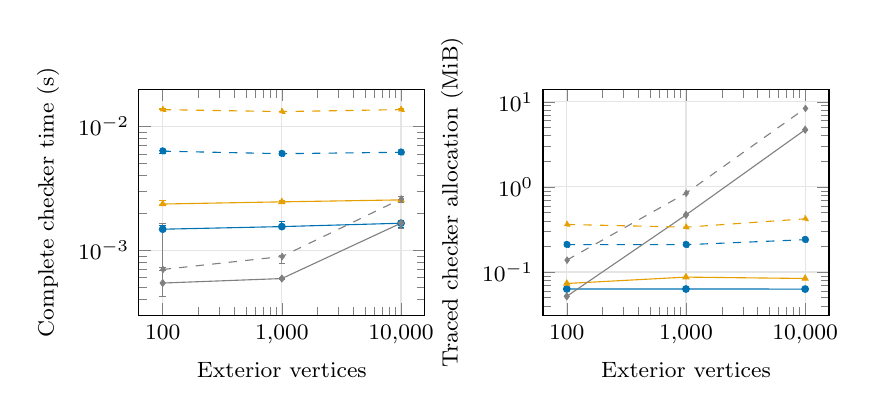
\begin{tikzpicture}
\begin{groupplot}[group style={group size=2 by 1,horizontal sep=15mm},width=.43\textwidth,height=1.75in,xmode=log,ymode=log,xtick={100,1000,10000},xticklabels={100,{1,000},{10,000}},xlabel={Exterior vertices},tick label style={font=\footnotesize},label style={font=\footnotesize},grid=major,grid style={gray!20}]
\nextgroupplot[ylabel={Complete checker time (s)}]
\addplot[color=proposalblue,solid,mark=*,mark size=1.2pt,error bars/.cd,y dir=both,y explicit] table[row sep=\\,x=x,y=y,y error minus=lo,y error plus=hi]{x y lo hi\\
100 0.00147900032 1.25728548e-07 0.000103874598\\
1000 0.00155283324 3.7999358e-05 0.000150999986\\
10000 0.00165308267 0.000121332705 1.39581971e-05\\
};
\addplot[color=referenceorange,solid,mark=triangle*,mark size=1.2pt,error bars/.cd,y dir=both,y explicit] table[row sep=\\,x=x,y=y,y error minus=lo,y error plus=hi]{x y lo hi\\
100 0.00236191694 2.47079879e-05 0.000145999715\\
1000 0.00245995773 5.11668622e-05 4.954217e-05\\
10000 0.00255141733 8.57091509e-05 2.34995969e-05\\
};
\addplot[color=gray,solid,mark=diamond*,mark size=1.2pt,error bars/.cd,y dir=both,y explicit] table[row sep=\\,x=x,y=y,y error minus=lo,y error plus=hi]{x y lo hi\\
100 0.000543707982 0.000119041186 0.00109558413\\
1000 0.000591000076 5.66709787e-06 7.83288851e-06\\
10000 0.0016561253 0.000152875204 6.52913004e-05\\
};
\addplot[color=proposalblue,dashed,mark=*,mark size=1.2pt,error bars/.cd,y dir=both,y explicit] table[row sep=\\,x=x,y=y,y error minus=lo,y error plus=hi]{x y lo hi\\
100 0.00631241733 0.000238792039 9.2915725e-05\\
1000 0.00602245796 0.000155750196 4.17088158e-05\\
10000 0.00618449971 0.00021683285 8.92500393e-05\\
};
\addplot[color=referenceorange,dashed,mark=triangle*,mark size=1.2pt,error bars/.cd,y dir=both,y explicit] table[row sep=\\,x=x,y=y,y error minus=lo,y error plus=hi]{x y lo hi\\
100 0.0136633748 3.1542033e-05 0.000305125024\\
1000 0.0131747918 1.06245279e-05 9.31243412e-05\\
10000 0.0136640002 4.93340194e-05 0.000171042047\\
};
\addplot[color=gray,dashed,mark=diamond*,mark size=1.2pt,error bars/.cd,y dir=both,y explicit] table[row sep=\\,x=x,y=y,y error minus=lo,y error plus=hi]{x y lo hi\\
100 0.000699541997 8.50111246e-06 2.41659582e-05\\
1000 0.0008896254 0.000101292506 2.35824846e-05\\
10000 0.0025932081 0.000141791999 0.00010158401\\
};
\nextgroupplot[ylabel={Traced checker allocation (MiB)}]
\addplot[color=proposalblue,solid,mark=*,mark size=1.2pt] coordinates {(100,0.0631608963) (1000,0.0630531311) (10000,0.063000679)};
\addplot[color=referenceorange,solid,mark=triangle*,mark size=1.2pt] coordinates {(100,0.073261261) (1000,0.0870714188) (10000,0.0838756561)};
\addplot[color=gray,solid,mark=diamond*,mark size=1.2pt] coordinates {(100,0.0517587662) (1000,0.469156265) (10000,4.70250225)};
\addplot[color=proposalblue,dashed,mark=*,mark size=1.2pt] coordinates {(100,0.20945549) (1000,0.209393501) (10000,0.239811897)};
\addplot[color=referenceorange,dashed,mark=triangle*,mark size=1.2pt] coordinates {(100,0.362134933) (1000,0.336591721) (10000,0.421858788)};
\addplot[color=gray,dashed,mark=diamond*,mark size=1.2pt] coordinates {(100,0.137942314) (1000,0.843913078) (10000,8.37305069)};
\end{groupplot}
\end{tikzpicture}
\caption{Fixed-core scaling. Circles: median certificate; triangles: full-pair certificate; diamonds: uncertified dense diagnostic. Time shows the median and range of three isolated, unprofiled repetitions; traced memory uses a separate repetition. Solid curves have $k=16$ and dashed curves $k=32$. Process RSS, including input and preparation, is reported separately.}\label{fig:scaling}
\end{figure*}
% END GENERATED SCALING FIGURE

\section{Complete Sequential-Pipeline Results}\label{app:v2-results}
The following figures and table retain every setting of the separately frozen
four-arm extension. Timing and exact modularity describe returned feasible
solutions. The three discovery seeds are fixed observations, and the one-,
three- and nine-call prefixes are correlated summaries. Observed ranges are
not confidence intervals. Original-graph objective evaluation and explicit
quality-matched denominators accompany all speedup comparisons.

% BEGIN RETAINED COMPLETE V2 COMPARISON TABLE
\begin{table*}[t]
\caption{Complete V2 descriptive comparison summary. Each row contains all 18 graph/resolution settings and 54 fixed discovery-seed observations. Speedups are constructed standalone $T_B/T_A$: the first range spans the 18 per-setting medians, and the count records medians above 1. Q counts are exact worse/equal/better outcomes for A versus B, out of 54. Matches require exact equal Q; their range uses every matched seed speedup, with its own non-null $n$ and no values if $n=0$. Prefixes $k$ are correlated summaries of the same nine calls. These are observed counts, not pooled population inference.}\label{tab:v2-prefixes}
\centering\small
\begin{tabular}{lcrrrrr}\toprule
Pair & $k$ & Speedup range & $>1$/18 & Q worse/equal/better & Matches/54 & Matched range ($n$)\\\midrule
D/U & 1 & 0.19--0.33 & 0/18 & 32/7/15 & 7/54 & 0.18--0.28 (7)\\
D/U & 3 & 0.32--0.54 & 0/18 & 31/4/19 & 4/54 & 0.33--0.41 (4)\\
D/U & 9 & 0.55--0.75 & 0/18 & 31/3/20 & 3/54 & 0.59--0.62 (3)\\
R/U & 1 & 0.13--0.33 & 0/18 & 21/6/27 & 6/54 & 0.20--0.24 (6)\\
R/U & 3 & 0.21--0.55 & 0/18 & 29/4/21 & 4/54 & 0.28--0.39 (4)\\
R/U & 9 & 0.38--0.75 & 0/18 & 25/2/27 & 2/54 & 0.40--0.63 (2)\\
RD/U & 1 & 0.10--0.25 & 0/18 & 26/7/21 & 7/54 & 0.10--0.19 (7)\\
RD/U & 3 & 0.17--0.43 & 0/18 & 34/4/16 & 4/54 & 0.23--0.32 (4)\\
RD/U & 9 & 0.32--0.64 & 0/18 & 32/2/20 & 2/54 & 0.37--0.56 (2)\\
D/R & 1 & 0.92--2.02 & 13/18 & 32/4/18 & 4/54 & 0.92--1.38 (4)\\
D/R & 3 & 0.91--1.84 & 12/18 & 31/4/19 & 4/54 & 0.91--1.45 (4)\\
D/R & 9 & 0.93--1.54 & 11/18 & 34/2/18 & 2/54 & 0.95--1.53 (2)\\
RD/R & 1 & 0.72--0.80 & 0/18 & 25/13/16 & 13/54 & 0.71--0.81 (13)\\
RD/R & 3 & 0.75--0.86 & 0/18 & 26/12/16 & 12/54 & 0.74--0.86 (12)\\
RD/R & 9 & 0.81--0.92 & 0/18 & 26/11/17 & 11/54 & 0.80--0.93 (11)\\
\bottomrule\end{tabular}
\end{table*}
% END RETAINED COMPLETE V2 COMPARISON TABLE

% BEGIN GENERATED tables/public-pipelines-v2/coverage-table.tex
\begin{table*}[t]
\caption{All 18 V2 graph/resolution coverage settings. Entries are median [minimum,maximum] over three fixed discovery seeds. The denominator is every original vertex. RD additional counts use its own freshly executed R prefix. The observed ranges are not confidence intervals.}\label{tab:v2-coverage}
\centering\small
\begin{tabular}{lcrrrr}\toprule
Graph & $\gamma$ & D removed (\%) & R removed (\%) & RD removed (\%) & RD additional vertices\\\midrule
GrQc & 1/2 & 35.1 [34.0,35.3] & 44.4 [44.3,44.6] & 49.5 [48.9,49.8] & 272 [237,273]\\
GrQc & 1 & 35.1 [34.0,35.3] & 42.4 [42.3,42.5] & 48.1 [47.7,48.5] & 308 [278,317]\\
GrQc & 2 & 34.7 [34.0,35.0] & 30.0 [30.0,30.2] & 39.9 [39.4,40.0] & 520 [479,524]\\
HepTh & 1/2 & 24.1 [23.9,24.4] & 34.8 [34.6,35.0] & 38.9 [38.8,39.0] & 393 [392,426]\\
HepTh & 1 & 24.1 [23.9,24.4] & 32.9 [32.6,33.0] & 37.2 [37.1,37.4] & 437 [421,461]\\
HepTh & 2 & 24.1 [23.9,24.4] & 18.0 [18.0,18.0] & 27.3 [27.3,27.6] & 921 [921,944]\\
Email & 1/2 & 1.7 [1.2,1.8] & 9.6 [9.6,9.6] & 9.6 [9.6,9.7] & 0 [0,1]\\
Email & 1 & 1.7 [1.2,1.8] & 9.6 [9.6,9.6] & 9.6 [9.6,9.7] & 0 [0,1]\\
Email & 2 & 1.7 [1.2,1.8] & 0.1 [0.1,0.1] & 1.8 [1.3,1.9] & 17 [12,18]\\
Facebook & 1/2 & 5.6 [5.6,5.7] & 4.3 [4.3,4.3] & 8.0 [8.0,8.1] & 147 [147,151]\\
Facebook & 1 & 5.5 [5.5,5.7] & 4.1 [4.1,4.1] & 7.8 [7.8,7.9] & 150 [150,154]\\
Facebook & 2 & 5.5 [5.3,5.6] & 2.2 [2.2,2.2] & 6.1 [6.1,6.2] & 159 [157,162]\\
CondMat & 1/2 & 21.9 [21.4,21.9] & 32.1 [32.1,32.1] & 36.4 [36.1,36.5] & 987 [932,1022]\\
CondMat & 1 & 21.9 [21.4,21.9] & 30.5 [30.4,30.5] & 35.0 [34.8,35.2] & 1034 [1008,1102]\\
CondMat & 2 & 21.9 [21.4,21.9] & 23.3 [23.3,23.3] & 30.2 [29.9,30.3] & 1587 [1523,1618]\\
Gnutella & 1/2 & 6.0 [5.4,6.1] & 27.7 [27.7,27.7] & 27.7 [27.7,27.7] & 0 [0,0]\\
Gnutella & 1 & 6.0 [5.4,6.1] & 27.7 [27.7,27.7] & 27.7 [27.7,27.7] & 0 [0,0]\\
Gnutella & 2 & 6.0 [5.4,6.1] & 0.5 [0.5,0.5] & 6.1 [5.5,6.1] & 355 [316,356]\\
\bottomrule\end{tabular}
\end{table*}
% END GENERATED tables/public-pipelines-v2/coverage-table.tex

% BEGIN GENERATED figures/public-pipelines-v2/rd-additional.tex
\begin{figure*}[t]
\centering
\begingroup
\definecolor{vTwoD}{HTML}{0072B2}
\definecolor{vTwoR}{HTML}{E69F00}
\definecolor{vTwoRD}{HTML}{6A7178}
\begin{tikzpicture}[x=0.000875in,y=.31in,every node/.style={font=\footnotesize}]
\node at (1000.0,6.1) {$\gamma=1/2$};
\draw[gray!20,line width=.3pt] (0.0,-.5) -- (0.0,5.5);
\node at (0.0,-.9) {0};
\draw[gray!20,line width=.3pt] (500.0,-.5) -- (500.0,5.5);
\node at (500.0,-.9) {500};
\draw[gray!20,line width=.3pt] (1000.0,-.5) -- (1000.0,5.5);
\node at (1000.0,-.9) {1000};
\draw[gray!20,line width=.3pt] (1500.0,-.5) -- (1500.0,5.5);
\node at (1500.0,-.9) {1500};
\draw[gray!20,line width=.3pt] (2000.0,-.5) -- (2000.0,5.5);
\node at (2000.0,-.9) {2000};
\node at (1000.0,-1.4) {Additional vertices removed};
\node[anchor=east] at (-80.0,5) {GrQc};
\draw[vTwoRD,line width=.7pt] (237.0,5) -- (273.0,5);
\draw[vTwoRD,line width=.7pt] (237.0,4.92) -- (237.0,5.08);
\draw[vTwoRD,line width=.7pt] (273.0,4.92) -- (273.0,5.08);
\fill[vTwoRD] (272.0,5) circle[radius=1.3pt];
\node[anchor=east] at (-80.0,4) {HepTh};
\draw[vTwoRD,line width=.7pt] (392.0,4) -- (426.0,4);
\draw[vTwoRD,line width=.7pt] (392.0,3.92) -- (392.0,4.08);
\draw[vTwoRD,line width=.7pt] (426.0,3.92) -- (426.0,4.08);
\fill[vTwoRD] (393.0,4) circle[radius=1.3pt];
\node[anchor=east] at (-80.0,3) {Email};
\draw[vTwoRD,line width=.7pt] (0.0,3) -- (1.0,3);
\draw[vTwoRD,line width=.7pt] (0.0,2.92) -- (0.0,3.08);
\draw[vTwoRD,line width=.7pt] (1.0,2.92) -- (1.0,3.08);
\fill[vTwoRD] (0.0,3) circle[radius=1.3pt];
\node[anchor=east] at (-80.0,2) {Facebook};
\draw[vTwoRD,line width=.7pt] (147.0,2) -- (151.0,2);
\draw[vTwoRD,line width=.7pt] (147.0,1.92) -- (147.0,2.08);
\draw[vTwoRD,line width=.7pt] (151.0,1.92) -- (151.0,2.08);
\fill[vTwoRD] (147.0,2) circle[radius=1.3pt];
\node[anchor=east] at (-80.0,1) {CondMat};
\draw[vTwoRD,line width=.7pt] (932.0,1) -- (1022.0,1);
\draw[vTwoRD,line width=.7pt] (932.0,0.92) -- (932.0,1.08);
\draw[vTwoRD,line width=.7pt] (1022.0,0.92) -- (1022.0,1.08);
\fill[vTwoRD] (987.0,1) circle[radius=1.3pt];
\node[anchor=east] at (-80.0,0) {Gnutella};
\draw[vTwoRD,line width=.7pt] (0.0,0) -- (0.0,0);
\draw[vTwoRD,line width=.7pt] (0.0,-0.08) -- (0.0,0.08);
\draw[vTwoRD,line width=.7pt] (0.0,-0.08) -- (0.0,0.08);
\fill[vTwoRD] (0.0,0) circle[radius=1.3pt];
\node at (3400.0,6.1) {$\gamma=1$};
\draw[gray!20,line width=.3pt] (2400.0,-.5) -- (2400.0,5.5);
\node at (2400.0,-.9) {0};
\draw[gray!20,line width=.3pt] (2900.0,-.5) -- (2900.0,5.5);
\node at (2900.0,-.9) {500};
\draw[gray!20,line width=.3pt] (3400.0,-.5) -- (3400.0,5.5);
\node at (3400.0,-.9) {1000};
\draw[gray!20,line width=.3pt] (3900.0,-.5) -- (3900.0,5.5);
\node at (3900.0,-.9) {1500};
\draw[gray!20,line width=.3pt] (4400.0,-.5) -- (4400.0,5.5);
\node at (4400.0,-.9) {2000};
\node at (3400.0,-1.4) {Additional vertices removed};
\draw[vTwoRD,line width=.7pt] (2678.0,5) -- (2717.0,5);
\draw[vTwoRD,line width=.7pt] (2678.0,4.92) -- (2678.0,5.08);
\draw[vTwoRD,line width=.7pt] (2717.0,4.92) -- (2717.0,5.08);
\fill[vTwoRD] (2708.0,5) circle[radius=1.3pt];
\draw[vTwoRD,line width=.7pt] (2821.0,4) -- (2861.0,4);
\draw[vTwoRD,line width=.7pt] (2821.0,3.92) -- (2821.0,4.08);
\draw[vTwoRD,line width=.7pt] (2861.0,3.92) -- (2861.0,4.08);
\fill[vTwoRD] (2837.0,4) circle[radius=1.3pt];
\draw[vTwoRD,line width=.7pt] (2400.0,3) -- (2401.0,3);
\draw[vTwoRD,line width=.7pt] (2400.0,2.92) -- (2400.0,3.08);
\draw[vTwoRD,line width=.7pt] (2401.0,2.92) -- (2401.0,3.08);
\fill[vTwoRD] (2400.0,3) circle[radius=1.3pt];
\draw[vTwoRD,line width=.7pt] (2550.0,2) -- (2554.0,2);
\draw[vTwoRD,line width=.7pt] (2550.0,1.92) -- (2550.0,2.08);
\draw[vTwoRD,line width=.7pt] (2554.0,1.92) -- (2554.0,2.08);
\fill[vTwoRD] (2550.0,2) circle[radius=1.3pt];
\draw[vTwoRD,line width=.7pt] (3408.0,1) -- (3502.0,1);
\draw[vTwoRD,line width=.7pt] (3408.0,0.92) -- (3408.0,1.08);
\draw[vTwoRD,line width=.7pt] (3502.0,0.92) -- (3502.0,1.08);
\fill[vTwoRD] (3434.0,1) circle[radius=1.3pt];
\draw[vTwoRD,line width=.7pt] (2400.0,0) -- (2400.0,0);
\draw[vTwoRD,line width=.7pt] (2400.0,-0.08) -- (2400.0,0.08);
\draw[vTwoRD,line width=.7pt] (2400.0,-0.08) -- (2400.0,0.08);
\fill[vTwoRD] (2400.0,0) circle[radius=1.3pt];
\node at (5800.0,6.1) {$\gamma=2$};
\draw[gray!20,line width=.3pt] (4800.0,-.5) -- (4800.0,5.5);
\node at (4800.0,-.9) {0};
\draw[gray!20,line width=.3pt] (5300.0,-.5) -- (5300.0,5.5);
\node at (5300.0,-.9) {500};
\draw[gray!20,line width=.3pt] (5800.0,-.5) -- (5800.0,5.5);
\node at (5800.0,-.9) {1000};
\draw[gray!20,line width=.3pt] (6300.0,-.5) -- (6300.0,5.5);
\node at (6300.0,-.9) {1500};
\draw[gray!20,line width=.3pt] (6800.0,-.5) -- (6800.0,5.5);
\node at (6800.0,-.9) {2000};
\node at (5800.0,-1.4) {Additional vertices removed};
\draw[vTwoRD,line width=.7pt] (5279.0,5) -- (5324.0,5);
\draw[vTwoRD,line width=.7pt] (5279.0,4.92) -- (5279.0,5.08);
\draw[vTwoRD,line width=.7pt] (5324.0,4.92) -- (5324.0,5.08);
\fill[vTwoRD] (5320.0,5) circle[radius=1.3pt];
\draw[vTwoRD,line width=.7pt] (5721.0,4) -- (5744.0,4);
\draw[vTwoRD,line width=.7pt] (5721.0,3.92) -- (5721.0,4.08);
\draw[vTwoRD,line width=.7pt] (5744.0,3.92) -- (5744.0,4.08);
\fill[vTwoRD] (5721.0,4) circle[radius=1.3pt];
\draw[vTwoRD,line width=.7pt] (4812.0,3) -- (4818.0,3);
\draw[vTwoRD,line width=.7pt] (4812.0,2.92) -- (4812.0,3.08);
\draw[vTwoRD,line width=.7pt] (4818.0,2.92) -- (4818.0,3.08);
\fill[vTwoRD] (4817.0,3) circle[radius=1.3pt];
\draw[vTwoRD,line width=.7pt] (4957.0,2) -- (4962.0,2);
\draw[vTwoRD,line width=.7pt] (4957.0,1.92) -- (4957.0,2.08);
\draw[vTwoRD,line width=.7pt] (4962.0,1.92) -- (4962.0,2.08);
\fill[vTwoRD] (4959.0,2) circle[radius=1.3pt];
\draw[vTwoRD,line width=.7pt] (6323.0,1) -- (6418.0,1);
\draw[vTwoRD,line width=.7pt] (6323.0,0.92) -- (6323.0,1.08);
\draw[vTwoRD,line width=.7pt] (6418.0,0.92) -- (6418.0,1.08);
\fill[vTwoRD] (6387.0,1) circle[radius=1.3pt];
\draw[vTwoRD,line width=.7pt] (5116.0,0) -- (5156.0,0);
\draw[vTwoRD,line width=.7pt] (5116.0,-0.08) -- (5116.0,0.08);
\draw[vTwoRD,line width=.7pt] (5156.0,-0.08) -- (5156.0,0.08);
\fill[vTwoRD] (5155.0,0) circle[radius=1.3pt];
\end{tikzpicture}
\endgroup
\caption{All RD additional vertex removals after its own freshly executed R prefix. Points show the median and whiskers the observed minimum and maximum over three fixed discovery seeds, on a shared vertex-count scale. These are not a structural-partition union or an extra solver run. Exact counts are retained in Table~\ref{tab:v2-coverage}.}\label{fig:v2-rd-additional}
\end{figure*}
% END GENERATED figures/public-pipelines-v2/rd-additional.tex

% BEGIN GENERATED figures/public-pipelines-v2/utility.tex
\begin{figure*}[t]
\centering
\begingroup
\definecolor{vTwoD}{HTML}{0072B2}
\definecolor{vTwoR}{HTML}{E69F00}
\definecolor{vTwoRD}{HTML}{6A7178}
\begin{tikzpicture}[x=.52in,y=.17in,every node/.style={font=\fontsize{8.2}{9}\selectfont}]
\node[anchor=east,font=\small\bfseries] at (-1.25,32.9) {D/U};
\node at (1.5,36.9) {$\gamma=1/2$};
\node[anchor=east] at (-.1,35.9) {GrQc};
\filldraw[fill=vTwoR!46.470443!white,draw=gray!15,line width=.25pt] (0.0,35.4) rectangle (1.0,36.4);
\node at (0.5,35.9) {0.19};
\filldraw[fill=vTwoR!31.09861!white,draw=gray!15,line width=.25pt] (1.0,35.4) rectangle (2.0,36.4);
\node at (1.5,35.9) {0.33};
\filldraw[fill=vTwoR!14.087707!white,draw=gray!15,line width=.25pt] (2.0,35.4) rectangle (3.0,36.4);
\node at (2.5,35.9) {0.61};
\node[anchor=east] at (-.1,34.9) {HepTh};
\filldraw[fill=vTwoR!40.559745!white,draw=gray!15,line width=.25pt] (0.0,34.4) rectangle (1.0,35.4);
\node at (0.5,34.9) {0.24};
\filldraw[fill=vTwoR!27.031604!white,draw=gray!15,line width=.25pt] (1.0,34.4) rectangle (2.0,35.4);
\node at (1.5,34.9) {0.38};
\filldraw[fill=vTwoR!13.333893!white,draw=gray!15,line width=.25pt] (2.0,34.4) rectangle (3.0,35.4);
\node at (2.5,34.9) {0.62};
\node[anchor=east] at (-.1,33.9) {Email};
\filldraw[fill=vTwoR!38.577507!white,draw=gray!15,line width=.25pt] (0.0,33.4) rectangle (1.0,34.4);
\node at (0.5,33.9) {0.25};
\filldraw[fill=vTwoR!27.687125!white,draw=gray!15,line width=.25pt] (1.0,33.4) rectangle (2.0,34.4);
\node at (1.5,33.9) {0.37};
\filldraw[fill=vTwoR!16.60787!white,draw=gray!15,line width=.25pt] (2.0,33.4) rectangle (3.0,34.4);
\node at (2.5,33.9) {0.55};
\node[anchor=east] at (-.1,32.9) {Facebook};
\filldraw[fill=vTwoR!37.497507!white,draw=gray!15,line width=.25pt] (0.0,32.4) rectangle (1.0,33.4);
\node at (0.5,32.9) {0.26};
\filldraw[fill=vTwoR!27.202226!white,draw=gray!15,line width=.25pt] (1.0,32.4) rectangle (2.0,33.4);
\node at (1.5,32.9) {0.38};
\filldraw[fill=vTwoR!15.589303!white,draw=gray!15,line width=.25pt] (2.0,32.4) rectangle (3.0,33.4);
\node at (2.5,32.9) {0.58};
\node[anchor=east] at (-.1,31.9) {CondMat};
\filldraw[fill=vTwoR!38.368188!white,draw=gray!15,line width=.25pt] (0.0,31.4) rectangle (1.0,32.4);
\node at (0.5,31.9) {0.26};
\filldraw[fill=vTwoR!26.64141!white,draw=gray!15,line width=.25pt] (1.0,31.4) rectangle (2.0,32.4);
\node at (1.5,31.9) {0.39};
\filldraw[fill=vTwoR!13.689164!white,draw=gray!15,line width=.25pt] (2.0,31.4) rectangle (3.0,32.4);
\node at (2.5,31.9) {0.62};
\node[anchor=east] at (-.1,30.9) {Gnutella};
\filldraw[fill=vTwoR!38.408073!white,draw=gray!15,line width=.25pt] (0.0,30.4) rectangle (1.0,31.4);
\node at (0.5,30.9) {0.26};
\filldraw[fill=vTwoR!27.340287!white,draw=gray!15,line width=.25pt] (1.0,30.4) rectangle (2.0,31.4);
\node at (1.5,30.9) {0.38};
\filldraw[fill=vTwoR!15.227057!white,draw=gray!15,line width=.25pt] (2.0,30.4) rectangle (3.0,31.4);
\node at (2.5,30.9) {0.58};
\node at (0.5,29.95) {1};
\node at (1.5,29.95) {3};
\node at (2.5,29.95) {9};
\node at (5.05,36.9) {$\gamma=1$};
\filldraw[fill=vTwoR!47.571138!white,draw=gray!15,line width=.25pt] (3.55,35.4) rectangle (4.55,36.4);
\node at (4.05,35.9) {0.19};
\filldraw[fill=vTwoR!31.317019!white,draw=gray!15,line width=.25pt] (4.55,35.4) rectangle (5.55,36.4);
\node at (5.05,35.9) {0.33};
\filldraw[fill=vTwoR!14.16954!white,draw=gray!15,line width=.25pt] (5.55,35.4) rectangle (6.55,36.4);
\node at (6.05,35.9) {0.61};
\filldraw[fill=vTwoR!41.354243!white,draw=gray!15,line width=.25pt] (3.55,34.4) rectangle (4.55,35.4);
\node at (4.05,34.9) {0.23};
\filldraw[fill=vTwoR!27.52474!white,draw=gray!15,line width=.25pt] (4.55,34.4) rectangle (5.55,35.4);
\node at (5.05,34.9) {0.38};
\filldraw[fill=vTwoR!12.833596!white,draw=gray!15,line width=.25pt] (5.55,34.4) rectangle (6.55,35.4);
\node at (6.05,34.9) {0.63};
\filldraw[fill=vTwoR!36.412633!white,draw=gray!15,line width=.25pt] (3.55,33.4) rectangle (4.55,34.4);
\node at (4.05,33.9) {0.28};
\filldraw[fill=vTwoR!26.759868!white,draw=gray!15,line width=.25pt] (4.55,33.4) rectangle (5.55,34.4);
\node at (5.05,33.9) {0.39};
\filldraw[fill=vTwoR!14.197699!white,draw=gray!15,line width=.25pt] (5.55,33.4) rectangle (6.55,34.4);
\node at (6.05,33.9) {0.60};
\filldraw[fill=vTwoR!38.907457!white,draw=gray!15,line width=.25pt] (3.55,32.4) rectangle (4.55,33.4);
\node at (4.05,32.9) {0.25};
\filldraw[fill=vTwoR!27.937332!white,draw=gray!15,line width=.25pt] (4.55,32.4) rectangle (5.55,33.4);
\node at (5.05,32.9) {0.37};
\filldraw[fill=vTwoR!15.434907!white,draw=gray!15,line width=.25pt] (5.55,32.4) rectangle (6.55,33.4);
\node at (6.05,32.9) {0.58};
\filldraw[fill=vTwoR!38.693091!white,draw=gray!15,line width=.25pt] (3.55,31.4) rectangle (4.55,32.4);
\node at (4.05,31.9) {0.25};
\filldraw[fill=vTwoR!26.878842!white,draw=gray!15,line width=.25pt] (4.55,31.4) rectangle (5.55,32.4);
\node at (5.05,31.9) {0.39};
\filldraw[fill=vTwoR!13.589274!white,draw=gray!15,line width=.25pt] (5.55,31.4) rectangle (6.55,32.4);
\node at (6.05,31.9) {0.62};
\filldraw[fill=vTwoR!36.439463!white,draw=gray!15,line width=.25pt] (3.55,30.4) rectangle (4.55,31.4);
\node at (4.05,30.9) {0.27};
\filldraw[fill=vTwoR!24.905742!white,draw=gray!15,line width=.25pt] (4.55,30.4) rectangle (5.55,31.4);
\node at (5.05,30.9) {0.41};
\filldraw[fill=vTwoR!13.65256!white,draw=gray!15,line width=.25pt] (5.55,30.4) rectangle (6.55,31.4);
\node at (6.05,30.9) {0.62};
\node at (4.05,29.95) {1};
\node at (5.05,29.95) {3};
\node at (6.05,29.95) {9};
\node at (8.6,36.9) {$\gamma=2$};
\filldraw[fill=vTwoR!44.836522!white,draw=gray!15,line width=.25pt] (7.1,35.4) rectangle (8.1,36.4);
\node at (7.6,35.9) {0.20};
\filldraw[fill=vTwoR!31.842039!white,draw=gray!15,line width=.25pt] (8.1,35.4) rectangle (9.1,36.4);
\node at (8.6,35.9) {0.32};
\filldraw[fill=vTwoR!14.78244!white,draw=gray!15,line width=.25pt] (9.1,35.4) rectangle (10.1,36.4);
\node at (9.6,35.9) {0.59};
\filldraw[fill=vTwoR!40.604656!white,draw=gray!15,line width=.25pt] (7.1,34.4) rectangle (8.1,35.4);
\node at (7.6,34.9) {0.24};
\filldraw[fill=vTwoR!27.860591!white,draw=gray!15,line width=.25pt] (8.1,34.4) rectangle (9.1,35.4);
\node at (8.6,34.9) {0.37};
\filldraw[fill=vTwoR!13.617264!white,draw=gray!15,line width=.25pt] (9.1,34.4) rectangle (10.1,35.4);
\node at (9.6,34.9) {0.62};
\filldraw[fill=vTwoR!37.450345!white,draw=gray!15,line width=.25pt] (7.1,33.4) rectangle (8.1,34.4);
\node at (7.6,33.9) {0.27};
\filldraw[fill=vTwoR!26.771459!white,draw=gray!15,line width=.25pt] (8.1,33.4) rectangle (9.1,34.4);
\node at (8.6,33.9) {0.39};
\filldraw[fill=vTwoR!14.05432!white,draw=gray!15,line width=.25pt] (9.1,33.4) rectangle (10.1,34.4);
\node at (9.6,33.9) {0.61};
\filldraw[fill=vTwoR!38.31848!white,draw=gray!15,line width=.25pt] (7.1,32.4) rectangle (8.1,33.4);
\node at (7.6,32.9) {0.26};
\filldraw[fill=vTwoR!26.08296!white,draw=gray!15,line width=.25pt] (8.1,32.4) rectangle (9.1,33.4);
\node at (8.6,32.9) {0.40};
\filldraw[fill=vTwoR!14.286002!white,draw=gray!15,line width=.25pt] (9.1,32.4) rectangle (10.1,33.4);
\node at (9.6,32.9) {0.60};
\filldraw[fill=vTwoR!38.819788!white,draw=gray!15,line width=.25pt] (7.1,31.4) rectangle (8.1,32.4);
\node at (7.6,31.9) {0.25};
\filldraw[fill=vTwoR!26.954268!white,draw=gray!15,line width=.25pt] (8.1,31.4) rectangle (9.1,32.4);
\node at (8.6,31.9) {0.38};
\filldraw[fill=vTwoR!14.285658!white,draw=gray!15,line width=.25pt] (9.1,31.4) rectangle (10.1,32.4);
\node at (9.6,31.9) {0.60};
\filldraw[fill=vTwoR!31.686795!white,draw=gray!15,line width=.25pt] (7.1,30.4) rectangle (8.1,31.4);
\node at (7.6,30.9) {0.33};
\filldraw[fill=vTwoR!17.414238!white,draw=gray!15,line width=.25pt] (8.1,30.4) rectangle (9.1,31.4);
\node at (8.6,30.9) {0.54};
\filldraw[fill=vTwoR!7.9954335!white,draw=gray!15,line width=.25pt] (9.1,30.4) rectangle (10.1,31.4);
\node at (9.6,30.9) {0.75};
\node at (7.6,29.95) {1};
\node at (8.6,29.95) {3};
\node at (9.6,29.95) {9};
\node[anchor=east,font=\small\bfseries] at (-1.25,25.299999999999997) {R/U};
\node[anchor=east] at (-.1,28.299999999999997) {GrQc};
\filldraw[fill=vTwoR!44.549417!white,draw=gray!15,line width=.25pt] (0.0,27.799999999999997) rectangle (1.0,28.799999999999997);
\node at (0.5,28.299999999999997) {0.21};
\filldraw[fill=vTwoR!28.964511!white,draw=gray!15,line width=.25pt] (1.0,27.799999999999997) rectangle (2.0,28.799999999999997);
\node at (1.5,28.299999999999997) {0.36};
\filldraw[fill=vTwoR!12.259544!white,draw=gray!15,line width=.25pt] (2.0,27.799999999999997) rectangle (3.0,28.799999999999997);
\node at (2.5,28.299999999999997) {0.65};
\node[anchor=east] at (-.1,27.299999999999997) {HepTh};
\filldraw[fill=vTwoR!42.382576!white,draw=gray!15,line width=.25pt] (0.0,26.799999999999997) rectangle (1.0,27.799999999999997);
\node at (0.5,27.299999999999997) {0.22};
\filldraw[fill=vTwoR!28.306968!white,draw=gray!15,line width=.25pt] (1.0,26.799999999999997) rectangle (2.0,27.799999999999997);
\node at (1.5,27.299999999999997) {0.37};
\filldraw[fill=vTwoR!12.949757!white,draw=gray!15,line width=.25pt] (2.0,26.799999999999997) rectangle (3.0,27.799999999999997);
\node at (2.5,27.299999999999997) {0.63};
\node[anchor=east] at (-.1,26.299999999999997) {Email};
\filldraw[fill=vTwoR!47.151193!white,draw=gray!15,line width=.25pt] (0.0,25.799999999999997) rectangle (1.0,26.799999999999997);
\node at (0.5,26.299999999999997) {0.19};
\filldraw[fill=vTwoR!34.888283!white,draw=gray!15,line width=.25pt] (1.0,25.799999999999997) rectangle (2.0,26.799999999999997);
\node at (1.5,26.299999999999997) {0.29};
\filldraw[fill=vTwoR!20.589757!white,draw=gray!15,line width=.25pt] (2.0,25.799999999999997) rectangle (3.0,26.799999999999997);
\node at (2.5,26.299999999999997) {0.48};
\node[anchor=east] at (-.1,25.299999999999997) {Facebook};
\filldraw[fill=vTwoR!57.149903!white,draw=gray!15,line width=.25pt] (0.0,24.799999999999997) rectangle (1.0,25.799999999999997);
\node at (0.5,25.299999999999997) {0.13};
\filldraw[fill=vTwoR!44.175489!white,draw=gray!15,line width=.25pt] (1.0,24.799999999999997) rectangle (2.0,25.799999999999997);
\node at (1.5,25.299999999999997) {0.21};
\filldraw[fill=vTwoR!27.458989!white,draw=gray!15,line width=.25pt] (2.0,24.799999999999997) rectangle (3.0,25.799999999999997);
\node at (2.5,25.299999999999997) {0.38};
\node[anchor=east] at (-.1,24.299999999999997) {CondMat};
\filldraw[fill=vTwoR!42.190877!white,draw=gray!15,line width=.25pt] (0.0,23.799999999999997) rectangle (1.0,24.799999999999997);
\node at (0.5,24.299999999999997) {0.22};
\filldraw[fill=vTwoR!29.040915!white,draw=gray!15,line width=.25pt] (1.0,23.799999999999997) rectangle (2.0,24.799999999999997);
\node at (1.5,24.299999999999997) {0.36};
\filldraw[fill=vTwoR!14.005063!white,draw=gray!15,line width=.25pt] (2.0,23.799999999999997) rectangle (3.0,24.799999999999997);
\node at (2.5,24.299999999999997) {0.61};
\node[anchor=east] at (-.1,23.299999999999997) {Gnutella};
\filldraw[fill=vTwoR!36.434855!white,draw=gray!15,line width=.25pt] (0.0,22.799999999999997) rectangle (1.0,23.799999999999997);
\node at (0.5,23.299999999999997) {0.27};
\filldraw[fill=vTwoR!25.16657!white,draw=gray!15,line width=.25pt] (1.0,22.799999999999997) rectangle (2.0,23.799999999999997);
\node at (1.5,23.299999999999997) {0.41};
\filldraw[fill=vTwoR!14.156447!white,draw=gray!15,line width=.25pt] (2.0,22.799999999999997) rectangle (3.0,23.799999999999997);
\node at (2.5,23.299999999999997) {0.61};
\node at (0.5,22.349999999999998) {1};
\node at (1.5,22.349999999999998) {3};
\node at (2.5,22.349999999999998) {9};
\filldraw[fill=vTwoR!45.172664!white,draw=gray!15,line width=.25pt] (3.55,27.799999999999997) rectangle (4.55,28.799999999999997);
\node at (4.05,28.299999999999997) {0.20};
\filldraw[fill=vTwoR!28.409198!white,draw=gray!15,line width=.25pt] (4.55,27.799999999999997) rectangle (5.55,28.799999999999997);
\node at (5.05,28.299999999999997) {0.37};
\filldraw[fill=vTwoR!12.906184!white,draw=gray!15,line width=.25pt] (5.55,27.799999999999997) rectangle (6.55,28.799999999999997);
\node at (6.05,28.299999999999997) {0.63};
\filldraw[fill=vTwoR!40.702206!white,draw=gray!15,line width=.25pt] (3.55,26.799999999999997) rectangle (4.55,27.799999999999997);
\node at (4.05,27.299999999999997) {0.24};
\filldraw[fill=vTwoR!26.499448!white,draw=gray!15,line width=.25pt] (4.55,26.799999999999997) rectangle (5.55,27.799999999999997);
\node at (5.05,27.299999999999997) {0.39};
\filldraw[fill=vTwoR!11.283791!white,draw=gray!15,line width=.25pt] (5.55,26.799999999999997) rectangle (6.55,27.799999999999997);
\node at (6.05,27.299999999999997) {0.67};
\filldraw[fill=vTwoR!45.429586!white,draw=gray!15,line width=.25pt] (3.55,25.799999999999997) rectangle (4.55,26.799999999999997);
\node at (4.05,26.299999999999997) {0.20};
\filldraw[fill=vTwoR!34.228762!white,draw=gray!15,line width=.25pt] (4.55,25.799999999999997) rectangle (5.55,26.799999999999997);
\node at (5.05,26.299999999999997) {0.30};
\filldraw[fill=vTwoR!20.609904!white,draw=gray!15,line width=.25pt] (5.55,25.799999999999997) rectangle (6.55,26.799999999999997);
\node at (6.05,26.299999999999997) {0.48};
\filldraw[fill=vTwoR!58.019656!white,draw=gray!15,line width=.25pt] (3.55,24.799999999999997) rectangle (4.55,25.799999999999997);
\node at (4.05,25.299999999999997) {0.13};
\filldraw[fill=vTwoR!44.114894!white,draw=gray!15,line width=.25pt] (4.55,24.799999999999997) rectangle (5.55,25.799999999999997);
\node at (5.05,25.299999999999997) {0.21};
\filldraw[fill=vTwoR!27.2483!white,draw=gray!15,line width=.25pt] (5.55,24.799999999999997) rectangle (6.55,25.799999999999997);
\node at (6.05,25.299999999999997) {0.38};
\filldraw[fill=vTwoR!42.956294!white,draw=gray!15,line width=.25pt] (3.55,23.799999999999997) rectangle (4.55,24.799999999999997);
\node at (4.05,24.299999999999997) {0.22};
\filldraw[fill=vTwoR!29.678813!white,draw=gray!15,line width=.25pt] (4.55,23.799999999999997) rectangle (5.55,24.799999999999997);
\node at (5.05,24.299999999999997) {0.35};
\filldraw[fill=vTwoR!14.148777!white,draw=gray!15,line width=.25pt] (5.55,23.799999999999997) rectangle (6.55,24.799999999999997);
\node at (6.05,24.299999999999997) {0.61};
\filldraw[fill=vTwoR!40.589914!white,draw=gray!15,line width=.25pt] (3.55,22.799999999999997) rectangle (4.55,23.799999999999997);
\node at (4.05,23.299999999999997) {0.24};
\filldraw[fill=vTwoR!35.541933!white,draw=gray!15,line width=.25pt] (4.55,22.799999999999997) rectangle (5.55,23.799999999999997);
\node at (5.05,23.299999999999997) {0.28};
\filldraw[fill=vTwoR!25.155697!white,draw=gray!15,line width=.25pt] (5.55,22.799999999999997) rectangle (6.55,23.799999999999997);
\node at (6.05,23.299999999999997) {0.41};
\node at (4.05,22.349999999999998) {1};
\node at (5.05,22.349999999999998) {3};
\node at (6.05,22.349999999999998) {9};
\filldraw[fill=vTwoR!44.433898!white,draw=gray!15,line width=.25pt] (7.1,27.799999999999997) rectangle (8.1,28.799999999999997);
\node at (7.6,28.299999999999997) {0.21};
\filldraw[fill=vTwoR!30.246908!white,draw=gray!15,line width=.25pt] (8.1,27.799999999999997) rectangle (9.1,28.799999999999997);
\node at (8.6,28.299999999999997) {0.34};
\filldraw[fill=vTwoR!14.166044!white,draw=gray!15,line width=.25pt] (9.1,27.799999999999997) rectangle (10.1,28.799999999999997);
\node at (9.6,28.299999999999997) {0.61};
\filldraw[fill=vTwoR!41.463348!white,draw=gray!15,line width=.25pt] (7.1,26.799999999999997) rectangle (8.1,27.799999999999997);
\node at (7.6,27.299999999999997) {0.23};
\filldraw[fill=vTwoR!28.367704!white,draw=gray!15,line width=.25pt] (8.1,26.799999999999997) rectangle (9.1,27.799999999999997);
\node at (8.6,27.299999999999997) {0.37};
\filldraw[fill=vTwoR!14.113974!white,draw=gray!15,line width=.25pt] (9.1,26.799999999999997) rectangle (10.1,27.799999999999997);
\node at (9.6,27.299999999999997) {0.61};
\filldraw[fill=vTwoR!44.805777!white,draw=gray!15,line width=.25pt] (7.1,25.799999999999997) rectangle (8.1,26.799999999999997);
\node at (7.6,26.299999999999997) {0.20};
\filldraw[fill=vTwoR!32.39701!white,draw=gray!15,line width=.25pt] (8.1,25.799999999999997) rectangle (9.1,26.799999999999997);
\node at (8.6,26.299999999999997) {0.32};
\filldraw[fill=vTwoR!17.920675!white,draw=gray!15,line width=.25pt] (9.1,25.799999999999997) rectangle (10.1,26.799999999999997);
\node at (9.6,26.299999999999997) {0.53};
\filldraw[fill=vTwoR!58.159067!white,draw=gray!15,line width=.25pt] (7.1,24.799999999999997) rectangle (8.1,25.799999999999997);
\node at (7.6,25.299999999999997) {0.13};
\filldraw[fill=vTwoR!43.26558!white,draw=gray!15,line width=.25pt] (8.1,24.799999999999997) rectangle (9.1,25.799999999999997);
\node at (8.6,25.299999999999997) {0.22};
\filldraw[fill=vTwoR!26.511527!white,draw=gray!15,line width=.25pt] (9.1,24.799999999999997) rectangle (10.1,25.799999999999997);
\node at (9.6,25.299999999999997) {0.39};
\filldraw[fill=vTwoR!42.283066!white,draw=gray!15,line width=.25pt] (7.1,23.799999999999997) rectangle (8.1,24.799999999999997);
\node at (7.6,24.299999999999997) {0.22};
\filldraw[fill=vTwoR!29.757406!white,draw=gray!15,line width=.25pt] (8.1,23.799999999999997) rectangle (9.1,24.799999999999997);
\node at (8.6,24.299999999999997) {0.35};
\filldraw[fill=vTwoR!15.665965!white,draw=gray!15,line width=.25pt] (9.1,23.799999999999997) rectangle (10.1,24.799999999999997);
\node at (9.6,24.299999999999997) {0.57};
\filldraw[fill=vTwoR!30.910618!white,draw=gray!15,line width=.25pt] (7.1,22.799999999999997) rectangle (8.1,23.799999999999997);
\node at (7.6,23.299999999999997) {0.33};
\filldraw[fill=vTwoR!16.861027!white,draw=gray!15,line width=.25pt] (8.1,22.799999999999997) rectangle (9.1,23.799999999999997);
\node at (8.6,23.299999999999997) {0.55};
\filldraw[fill=vTwoR!8.0608654!white,draw=gray!15,line width=.25pt] (9.1,22.799999999999997) rectangle (10.1,23.799999999999997);
\node at (9.6,23.299999999999997) {0.75};
\node at (7.6,22.349999999999998) {1};
\node at (8.6,22.349999999999998) {3};
\node at (9.6,22.349999999999998) {9};
\node[anchor=east,font=\small\bfseries] at (-1.25,17.7) {RD/U};
\node[anchor=east] at (-.1,20.7) {GrQc};
\filldraw[fill=vTwoR!50.93379!white,draw=gray!15,line width=.25pt] (0.0,20.2) rectangle (1.0,21.2);
\node at (0.5,20.7) {0.16};
\filldraw[fill=vTwoR!34.32476!white,draw=gray!15,line width=.25pt] (1.0,20.2) rectangle (2.0,21.2);
\node at (1.5,20.7) {0.30};
\filldraw[fill=vTwoR!15.869424!white,draw=gray!15,line width=.25pt] (2.0,20.2) rectangle (3.0,21.2);
\node at (2.5,20.7) {0.57};
\node[anchor=east] at (-.1,19.7) {HepTh};
\filldraw[fill=vTwoR!49.062774!white,draw=gray!15,line width=.25pt] (0.0,19.2) rectangle (1.0,20.2);
\node at (0.5,19.7) {0.18};
\filldraw[fill=vTwoR!33.730947!white,draw=gray!15,line width=.25pt] (1.0,19.2) rectangle (2.0,20.2);
\node at (1.5,19.7) {0.30};
\filldraw[fill=vTwoR!16.615702!white,draw=gray!15,line width=.25pt] (2.0,19.2) rectangle (3.0,20.2);
\node at (2.5,19.7) {0.55};
\node[anchor=east] at (-.1,18.7) {Email};
\filldraw[fill=vTwoR!56.0117!white,draw=gray!15,line width=.25pt] (0.0,18.2) rectangle (1.0,19.2);
\node at (0.5,18.7) {0.14};
\filldraw[fill=vTwoR!42.930853!white,draw=gray!15,line width=.25pt] (1.0,18.2) rectangle (2.0,19.2);
\node at (1.5,18.7) {0.22};
\filldraw[fill=vTwoR!26.404676!white,draw=gray!15,line width=.25pt] (2.0,18.2) rectangle (3.0,19.2);
\node at (2.5,18.7) {0.39};
\node[anchor=east] at (-.1,17.7) {Facebook};
\filldraw[fill=vTwoR!63.613577!white,draw=gray!15,line width=.25pt] (0.0,17.2) rectangle (1.0,18.2);
\node at (0.5,17.7) {0.10};
\filldraw[fill=vTwoR!50.212883!white,draw=gray!15,line width=.25pt] (1.0,17.2) rectangle (2.0,18.2);
\node at (1.5,17.7) {0.17};
\filldraw[fill=vTwoR!31.966535!white,draw=gray!15,line width=.25pt] (2.0,17.2) rectangle (3.0,18.2);
\node at (2.5,17.7) {0.32};
\node[anchor=east] at (-.1,16.7) {CondMat};
\filldraw[fill=vTwoR!48.77764!white,draw=gray!15,line width=.25pt] (0.0,16.2) rectangle (1.0,17.2);
\node at (0.5,16.7) {0.18};
\filldraw[fill=vTwoR!34.791177!white,draw=gray!15,line width=.25pt] (1.0,16.2) rectangle (2.0,17.2);
\node at (1.5,16.7) {0.29};
\filldraw[fill=vTwoR!17.405466!white,draw=gray!15,line width=.25pt] (2.0,16.2) rectangle (3.0,17.2);
\node at (2.5,16.7) {0.54};
\node[anchor=east] at (-.1,15.7) {Gnutella};
\filldraw[fill=vTwoR!44.001297!white,draw=gray!15,line width=.25pt] (0.0,15.2) rectangle (1.0,16.2);
\node at (0.5,15.7) {0.21};
\filldraw[fill=vTwoR!31.369999!white,draw=gray!15,line width=.25pt] (1.0,15.2) rectangle (2.0,16.2);
\node at (1.5,15.7) {0.33};
\filldraw[fill=vTwoR!18.446283!white,draw=gray!15,line width=.25pt] (2.0,15.2) rectangle (3.0,16.2);
\node at (2.5,15.7) {0.52};
\node at (0.5,14.75) {1};
\node at (1.5,14.75) {3};
\node at (2.5,14.75) {9};
\filldraw[fill=vTwoR!52.329651!white,draw=gray!15,line width=.25pt] (3.55,20.2) rectangle (4.55,21.2);
\node at (4.05,20.7) {0.16};
\filldraw[fill=vTwoR!34.856973!white,draw=gray!15,line width=.25pt] (4.55,20.2) rectangle (5.55,21.2);
\node at (5.05,20.7) {0.29};
\filldraw[fill=vTwoR!16.510876!white,draw=gray!15,line width=.25pt] (5.55,20.2) rectangle (6.55,21.2);
\node at (6.05,20.7) {0.56};
\filldraw[fill=vTwoR!48.698125!white,draw=gray!15,line width=.25pt] (3.55,19.2) rectangle (4.55,20.2);
\node at (4.05,19.7) {0.18};
\filldraw[fill=vTwoR!33.191127!white,draw=gray!15,line width=.25pt] (4.55,19.2) rectangle (5.55,20.2);
\node at (5.05,19.7) {0.31};
\filldraw[fill=vTwoR!15.648298!white,draw=gray!15,line width=.25pt] (5.55,19.2) rectangle (6.55,20.2);
\node at (6.05,19.7) {0.57};
\filldraw[fill=vTwoR!54.308277!white,draw=gray!15,line width=.25pt] (3.55,18.2) rectangle (4.55,19.2);
\node at (4.05,18.7) {0.15};
\filldraw[fill=vTwoR!42.015431!white,draw=gray!15,line width=.25pt] (4.55,18.2) rectangle (5.55,19.2);
\node at (5.05,18.7) {0.23};
\filldraw[fill=vTwoR!25.846385!white,draw=gray!15,line width=.25pt] (5.55,18.2) rectangle (6.55,19.2);
\node at (6.05,18.7) {0.40};
\filldraw[fill=vTwoR!64.335029!white,draw=gray!15,line width=.25pt] (3.55,17.2) rectangle (4.55,18.2);
\node at (4.05,17.7) {0.10};
\filldraw[fill=vTwoR!49.897182!white,draw=gray!15,line width=.25pt] (4.55,17.2) rectangle (5.55,18.2);
\node at (5.05,17.7) {0.17};
\filldraw[fill=vTwoR!31.467172!white,draw=gray!15,line width=.25pt] (5.55,17.2) rectangle (6.55,18.2);
\node at (6.05,17.7) {0.33};
\filldraw[fill=vTwoR!49.860017!white,draw=gray!15,line width=.25pt] (3.55,16.2) rectangle (4.55,17.2);
\node at (4.05,16.7) {0.17};
\filldraw[fill=vTwoR!35.406743!white,draw=gray!15,line width=.25pt] (4.55,16.2) rectangle (5.55,17.2);
\node at (5.05,16.7) {0.28};
\filldraw[fill=vTwoR!17.5558!white,draw=gray!15,line width=.25pt] (5.55,16.2) rectangle (6.55,17.2);
\node at (6.05,16.7) {0.54};
\filldraw[fill=vTwoR!46.907818!white,draw=gray!15,line width=.25pt] (3.55,15.2) rectangle (4.55,16.2);
\node at (4.05,15.7) {0.19};
\filldraw[fill=vTwoR!39.852363!white,draw=gray!15,line width=.25pt] (4.55,15.2) rectangle (5.55,16.2);
\node at (5.05,15.7) {0.24};
\filldraw[fill=vTwoR!27.660844!white,draw=gray!15,line width=.25pt] (5.55,15.2) rectangle (6.55,16.2);
\node at (6.05,15.7) {0.38};
\node at (4.05,14.75) {1};
\node at (5.05,14.75) {3};
\node at (6.05,14.75) {9};
\filldraw[fill=vTwoR!51.410835!white,draw=gray!15,line width=.25pt] (7.1,20.2) rectangle (8.1,21.2);
\node at (7.6,20.7) {0.16};
\filldraw[fill=vTwoR!37.159869!white,draw=gray!15,line width=.25pt] (8.1,20.2) rectangle (9.1,21.2);
\node at (8.6,20.7) {0.27};
\filldraw[fill=vTwoR!18.468296!white,draw=gray!15,line width=.25pt] (9.1,20.2) rectangle (10.1,21.2);
\node at (9.6,20.7) {0.52};
\filldraw[fill=vTwoR!49.26335!white,draw=gray!15,line width=.25pt] (7.1,19.2) rectangle (8.1,20.2);
\node at (7.6,19.7) {0.17};
\filldraw[fill=vTwoR!36.128271!white,draw=gray!15,line width=.25pt] (8.1,19.2) rectangle (9.1,20.2);
\node at (8.6,19.7) {0.28};
\filldraw[fill=vTwoR!19.007324!white,draw=gray!15,line width=.25pt] (9.1,19.2) rectangle (10.1,20.2);
\node at (9.6,19.7) {0.51};
\filldraw[fill=vTwoR!53.979625!white,draw=gray!15,line width=.25pt] (7.1,18.2) rectangle (8.1,19.2);
\node at (7.6,18.7) {0.15};
\filldraw[fill=vTwoR!41.627468!white,draw=gray!15,line width=.25pt] (8.1,18.2) rectangle (9.1,19.2);
\node at (8.6,18.7) {0.23};
\filldraw[fill=vTwoR!24.267976!white,draw=gray!15,line width=.25pt] (9.1,18.2) rectangle (10.1,19.2);
\node at (9.6,18.7) {0.42};
\filldraw[fill=vTwoR!65!white,draw=gray!15,line width=.25pt] (7.1,17.2) rectangle (8.1,18.2);
\node at (7.6,17.7) {0.10};
\filldraw[fill=vTwoR!49.45203!white,draw=gray!15,line width=.25pt] (8.1,17.2) rectangle (9.1,18.2);
\node at (8.6,17.7) {0.17};
\filldraw[fill=vTwoR!31.075993!white,draw=gray!15,line width=.25pt] (9.1,17.2) rectangle (10.1,18.2);
\node at (9.6,17.7) {0.33};
\filldraw[fill=vTwoR!49.248791!white,draw=gray!15,line width=.25pt] (7.1,16.2) rectangle (8.1,17.2);
\node at (7.6,16.7) {0.17};
\filldraw[fill=vTwoR!35.66919!white,draw=gray!15,line width=.25pt] (8.1,16.2) rectangle (9.1,17.2);
\node at (8.6,16.7) {0.28};
\filldraw[fill=vTwoR!19.615721!white,draw=gray!15,line width=.25pt] (9.1,16.2) rectangle (10.1,17.2);
\node at (9.6,16.7) {0.50};
\filldraw[fill=vTwoR!38.627327!white,draw=gray!15,line width=.25pt] (7.1,15.2) rectangle (8.1,16.2);
\node at (7.6,15.7) {0.25};
\filldraw[fill=vTwoR!23.81523!white,draw=gray!15,line width=.25pt] (8.1,15.2) rectangle (9.1,16.2);
\node at (8.6,15.7) {0.43};
\filldraw[fill=vTwoR!12.777813!white,draw=gray!15,line width=.25pt] (9.1,15.2) rectangle (10.1,16.2);
\node at (9.6,15.7) {0.64};
\node at (7.6,14.75) {1};
\node at (8.6,14.75) {3};
\node at (9.6,14.75) {9};
\node[anchor=east,font=\small\bfseries] at (-1.25,10.1) {D/R};
\node[anchor=east] at (-.1,13.1) {GrQc};
\filldraw[fill=vTwoR!1.8685654!white,draw=gray!15,line width=.25pt] (0.0,12.6) rectangle (1.0,13.6);
\node at (0.5,13.1) {0.94};
\filldraw[fill=vTwoR!1.7740798!white,draw=gray!15,line width=.25pt] (1.0,12.6) rectangle (2.0,13.6);
\node at (1.5,13.1) {0.94};
\filldraw[fill=vTwoR!1.9198931!white,draw=gray!15,line width=.25pt] (2.0,12.6) rectangle (3.0,13.6);
\node at (2.5,13.1) {0.93};
\node[anchor=east] at (-.1,12.1) {HepTh};
\filldraw[fill=vTwoD!1.8075019!white,draw=gray!15,line width=.25pt] (0.0,11.6) rectangle (1.0,12.6);
\node at (0.5,12.1) {1.07};
\filldraw[fill=vTwoD!1.2753638!white,draw=gray!15,line width=.25pt] (1.0,11.6) rectangle (2.0,12.6);
\node at (1.5,12.1) {1.05};
\filldraw[fill=vTwoR!0.38413615!white,draw=gray!15,line width=.25pt] (2.0,11.6) rectangle (3.0,12.6);
\node at (2.5,12.1) {0.99};
\node[anchor=east] at (-.1,11.1) {Email};
\filldraw[fill=vTwoD!8.5736858!white,draw=gray!15,line width=.25pt] (0.0,10.6) rectangle (1.0,11.6);
\node at (0.5,11.1) {1.36};
\filldraw[fill=vTwoD!7.3943527!white,draw=gray!15,line width=.25pt] (1.0,10.6) rectangle (2.0,11.6);
\node at (1.5,11.1) {1.30};
\filldraw[fill=vTwoD!5.4288191!white,draw=gray!15,line width=.25pt] (2.0,10.6) rectangle (3.0,11.6);
\node at (2.5,11.1) {1.21};
\node[anchor=east] at (-.1,10.1) {Facebook};
\filldraw[fill=vTwoD!19.882565!white,draw=gray!15,line width=.25pt] (0.0,9.6) rectangle (1.0,10.6);
\node at (0.5,10.1) {2.02};
\filldraw[fill=vTwoD!16.973264!white,draw=gray!15,line width=.25pt] (1.0,9.6) rectangle (2.0,10.6);
\node at (1.5,10.1) {1.83};
\filldraw[fill=vTwoD!11.88242!white,draw=gray!15,line width=.25pt] (2.0,9.6) rectangle (3.0,10.6);
\node at (2.5,10.1) {1.52};
\node[anchor=east] at (-.1,9.1) {CondMat};
\filldraw[fill=vTwoD!3.9452795!white,draw=gray!15,line width=.25pt] (0.0,8.6) rectangle (1.0,9.6);
\node at (0.5,9.1) {1.15};
\filldraw[fill=vTwoD!2.3995049!white,draw=gray!15,line width=.25pt] (1.0,8.6) rectangle (2.0,9.6);
\node at (1.5,9.1) {1.09};
\filldraw[fill=vTwoD!0.6233961!white,draw=gray!15,line width=.25pt] (2.0,8.6) rectangle (3.0,9.6);
\node at (2.5,9.1) {1.02};
\node[anchor=east] at (-.1,8.1) {Gnutella};
\filldraw[fill=vTwoR!1.9183423!white,draw=gray!15,line width=.25pt] (0.0,7.6) rectangle (1.0,8.6);
\node at (0.5,8.1) {0.93};
\filldraw[fill=vTwoR!2.1737172!white,draw=gray!15,line width=.25pt] (1.0,7.6) rectangle (2.0,8.6);
\node at (1.5,8.1) {0.93};
\filldraw[fill=vTwoR!1.0706096!white,draw=gray!15,line width=.25pt] (2.0,7.6) rectangle (3.0,8.6);
\node at (2.5,8.1) {0.96};
\node at (0.5,7.1499999999999995) {1};
\node at (1.5,7.1499999999999995) {3};
\node at (2.5,7.1499999999999995) {9};
\filldraw[fill=vTwoR!2.3724429!white,draw=gray!15,line width=.25pt] (3.55,12.6) rectangle (4.55,13.6);
\node at (4.05,13.1) {0.92};
\filldraw[fill=vTwoR!2.6922638!white,draw=gray!15,line width=.25pt] (4.55,12.6) rectangle (5.55,13.6);
\node at (5.05,13.1) {0.91};
\filldraw[fill=vTwoR!1.3373423!white,draw=gray!15,line width=.25pt] (5.55,12.6) rectangle (6.55,13.6);
\node at (6.05,13.1) {0.95};
\filldraw[fill=vTwoD!0.39322527!white,draw=gray!15,line width=.25pt] (3.55,11.6) rectangle (4.55,12.6);
\node at (4.05,12.1) {1.01};
\filldraw[fill=vTwoR!1.0252925!white,draw=gray!15,line width=.25pt] (4.55,11.6) rectangle (5.55,12.6);
\node at (5.05,12.1) {0.96};
\filldraw[fill=vTwoR!1.549805!white,draw=gray!15,line width=.25pt] (5.55,11.6) rectangle (6.55,12.6);
\node at (6.05,12.1) {0.95};
\filldraw[fill=vTwoD!8.9367858!white,draw=gray!15,line width=.25pt] (3.55,10.6) rectangle (4.55,11.6);
\node at (4.05,11.1) {1.37};
\filldraw[fill=vTwoD!7.559418!white,draw=gray!15,line width=.25pt] (4.55,10.6) rectangle (5.55,11.6);
\node at (5.05,11.1) {1.31};
\filldraw[fill=vTwoD!5.873158!white,draw=gray!15,line width=.25pt] (5.55,10.6) rectangle (6.55,11.6);
\node at (6.05,11.1) {1.23};
\filldraw[fill=vTwoD!19.469823!white,draw=gray!15,line width=.25pt] (3.55,9.6) rectangle (4.55,10.6);
\node at (4.05,10.1) {1.99};
\filldraw[fill=vTwoD!16.177562!white,draw=gray!15,line width=.25pt] (4.55,9.6) rectangle (5.55,10.6);
\node at (5.05,10.1) {1.77};
\filldraw[fill=vTwoD!11.823806!white,draw=gray!15,line width=.25pt] (5.55,9.6) rectangle (6.55,10.6);
\node at (6.05,10.1) {1.52};
\filldraw[fill=vTwoD!3.6653437!white,draw=gray!15,line width=.25pt] (3.55,8.6) rectangle (4.55,9.6);
\node at (4.05,9.1) {1.14};
\filldraw[fill=vTwoD!2.7999707!white,draw=gray!15,line width=.25pt] (4.55,8.6) rectangle (5.55,9.6);
\node at (5.05,9.1) {1.10};
\filldraw[fill=vTwoD!1.0101509!white,draw=gray!15,line width=.25pt] (5.55,8.6) rectangle (6.55,9.6);
\node at (6.05,9.1) {1.04};
\filldraw[fill=vTwoD!4.3748826!white,draw=gray!15,line width=.25pt] (3.55,7.6) rectangle (4.55,8.6);
\node at (4.05,8.1) {1.17};
\filldraw[fill=vTwoD!10.666972!white,draw=gray!15,line width=.25pt] (4.55,7.6) rectangle (5.55,8.6);
\node at (5.05,8.1) {1.46};
\filldraw[fill=vTwoD!11.914379!white,draw=gray!15,line width=.25pt] (5.55,7.6) rectangle (6.55,8.6);
\node at (6.05,8.1) {1.53};
\node at (4.05,7.1499999999999995) {1};
\node at (5.05,7.1499999999999995) {3};
\node at (6.05,7.1499999999999995) {9};
\filldraw[fill=vTwoR!0.62030031!white,draw=gray!15,line width=.25pt] (7.1,12.6) rectangle (8.1,13.6);
\node at (7.6,13.1) {0.98};
\filldraw[fill=vTwoR!1.0627583!white,draw=gray!15,line width=.25pt] (8.1,12.6) rectangle (9.1,13.6);
\node at (8.6,13.1) {0.96};
\filldraw[fill=vTwoR!0.41000576!white,draw=gray!15,line width=.25pt] (9.1,12.6) rectangle (10.1,13.6);
\node at (9.6,13.1) {0.99};
\filldraw[fill=vTwoD!0.28972862!white,draw=gray!15,line width=.25pt] (7.1,11.6) rectangle (8.1,12.6);
\node at (7.6,12.1) {1.01};
\filldraw[fill=vTwoD!0.76663012!white,draw=gray!15,line width=.25pt] (8.1,11.6) rectangle (9.1,12.6);
\node at (8.6,12.1) {1.03};
\filldraw[fill=vTwoD!0.53856994!white,draw=gray!15,line width=.25pt] (9.1,11.6) rectangle (10.1,12.6);
\node at (9.6,12.1) {1.02};
\filldraw[fill=vTwoD!7.3554318!white,draw=gray!15,line width=.25pt] (7.1,10.6) rectangle (8.1,11.6);
\node at (7.6,11.1) {1.30};
\filldraw[fill=vTwoD!5.8394423!white,draw=gray!15,line width=.25pt] (8.1,10.6) rectangle (9.1,11.6);
\node at (8.6,11.1) {1.23};
\filldraw[fill=vTwoD!3.7423546!white,draw=gray!15,line width=.25pt] (9.1,10.6) rectangle (10.1,11.6);
\node at (9.6,11.1) {1.14};
\filldraw[fill=vTwoD!19.697247!white,draw=gray!15,line width=.25pt] (7.1,9.6) rectangle (8.1,10.6);
\node at (7.6,10.1) {2.01};
\filldraw[fill=vTwoD!17.18262!white,draw=gray!15,line width=.25pt] (8.1,9.6) rectangle (9.1,10.6);
\node at (8.6,10.1) {1.84};
\filldraw[fill=vTwoD!12.225525!white,draw=gray!15,line width=.25pt] (9.1,9.6) rectangle (10.1,10.6);
\node at (9.6,10.1) {1.54};
\filldraw[fill=vTwoD!4.0489381!white,draw=gray!15,line width=.25pt] (7.1,8.6) rectangle (8.1,9.6);
\node at (7.6,9.1) {1.15};
\filldraw[fill=vTwoD!2.9154709!white,draw=gray!15,line width=.25pt] (8.1,8.6) rectangle (9.1,9.6);
\node at (8.6,9.1) {1.11};
\filldraw[fill=vTwoD!1.1265447!white,draw=gray!15,line width=.25pt] (9.1,8.6) rectangle (10.1,9.6);
\node at (9.6,9.1) {1.04};
\filldraw[fill=vTwoR!0.77617613!white,draw=gray!15,line width=.25pt] (7.1,7.6) rectangle (8.1,8.6);
\node at (7.6,8.1) {0.97};
\filldraw[fill=vTwoR!0.70890371!white,draw=gray!15,line width=.25pt] (8.1,7.6) rectangle (9.1,8.6);
\node at (8.6,8.1) {0.98};
\filldraw[fill=vTwoR!0.22648842!white,draw=gray!15,line width=.25pt] (9.1,7.6) rectangle (10.1,8.6);
\node at (9.6,8.1) {0.99};
\node at (7.6,7.1499999999999995) {1};
\node at (8.6,7.1499999999999995) {3};
\node at (9.6,7.1499999999999995) {9};
\node[anchor=east,font=\small\bfseries] at (-1.25,2.5) {RD/R};
\node[anchor=east] at (-.1,5.5) {GrQc};
\filldraw[fill=vTwoR!6.6494489!white,draw=gray!15,line width=.25pt] (0.0,5.0) rectangle (1.0,6.0);
\node at (0.5,5.5) {0.79};
\filldraw[fill=vTwoR!5.5337611!white,draw=gray!15,line width=.25pt] (1.0,5.0) rectangle (2.0,6.0);
\node at (1.5,5.5) {0.82};
\filldraw[fill=vTwoR!4.1730592!white,draw=gray!15,line width=.25pt] (2.0,5.0) rectangle (3.0,6.0);
\node at (2.5,5.5) {0.86};
\node[anchor=east] at (-.1,4.5) {HepTh};
\filldraw[fill=vTwoR!6.2310405!white,draw=gray!15,line width=.25pt] (0.0,4.0) rectangle (1.0,5.0);
\node at (0.5,4.5) {0.80};
\filldraw[fill=vTwoR!5.3884089!white,draw=gray!15,line width=.25pt] (1.0,4.0) rectangle (2.0,5.0);
\node at (1.5,4.5) {0.83};
\filldraw[fill=vTwoR!3.792734!white,draw=gray!15,line width=.25pt] (2.0,4.0) rectangle (3.0,5.0);
\node at (2.5,4.5) {0.87};
\node[anchor=east] at (-.1,3.5) {Email};
\filldraw[fill=vTwoR!9.148029!white,draw=gray!15,line width=.25pt] (0.0,3.0) rectangle (1.0,4.0);
\node at (0.5,3.5) {0.72};
\filldraw[fill=vTwoR!8.1989633!white,draw=gray!15,line width=.25pt] (1.0,3.0) rectangle (2.0,4.0);
\node at (1.5,3.5) {0.75};
\filldraw[fill=vTwoR!5.8149191!white,draw=gray!15,line width=.25pt] (2.0,3.0) rectangle (3.0,4.0);
\node at (2.5,3.5) {0.81};
\node[anchor=east] at (-.1,2.5) {Facebook};
\filldraw[fill=vTwoR!6.4782243!white,draw=gray!15,line width=.25pt] (0.0,2.0) rectangle (1.0,3.0);
\node at (0.5,2.5) {0.79};
\filldraw[fill=vTwoR!6.037393!white,draw=gray!15,line width=.25pt] (1.0,2.0) rectangle (2.0,3.0);
\node at (1.5,2.5) {0.81};
\filldraw[fill=vTwoR!4.487138!white,draw=gray!15,line width=.25pt] (2.0,2.0) rectangle (3.0,3.0);
\node at (2.5,2.5) {0.85};
\node[anchor=east] at (-.1,1.5) {CondMat};
\filldraw[fill=vTwoR!6.5983861!white,draw=gray!15,line width=.25pt] (0.0,1.0) rectangle (1.0,2.0);
\node at (0.5,1.5) {0.79};
\filldraw[fill=vTwoR!5.7502616!white,draw=gray!15,line width=.25pt] (1.0,1.0) rectangle (2.0,2.0);
\node at (1.5,1.5) {0.82};
\filldraw[fill=vTwoR!3.7083387!white,draw=gray!15,line width=.25pt] (2.0,1.0) rectangle (3.0,2.0);
\node at (2.5,1.5) {0.88};
\node[anchor=east] at (-.1,0.5) {Gnutella};
\filldraw[fill=vTwoR!7.922852!white,draw=gray!15,line width=.25pt] (0.0,0.0) rectangle (1.0,1.0);
\node at (0.5,0.5) {0.76};
\filldraw[fill=vTwoR!6.3167969!white,draw=gray!15,line width=.25pt] (1.0,0.0) rectangle (2.0,1.0);
\node at (1.5,0.5) {0.80};
\filldraw[fill=vTwoR!4.2898351!white,draw=gray!15,line width=.25pt] (2.0,0.0) rectangle (3.0,1.0);
\node at (2.5,0.5) {0.86};
\node at (0.5,-0.45) {1};
\node at (1.5,-0.45) {3};
\node at (2.5,-0.45) {9};
\filldraw[fill=vTwoR!6.929497!white,draw=gray!15,line width=.25pt] (3.55,5.0) rectangle (4.55,6.0);
\node at (4.05,5.5) {0.78};
\filldraw[fill=vTwoR!6.3684733!white,draw=gray!15,line width=.25pt] (4.55,5.0) rectangle (5.55,6.0);
\node at (5.05,5.5) {0.80};
\filldraw[fill=vTwoR!3.6786778!white,draw=gray!15,line width=.25pt] (5.55,5.0) rectangle (6.55,6.0);
\node at (6.05,5.5) {0.88};
\filldraw[fill=vTwoR!6.9469399!white,draw=gray!15,line width=.25pt] (3.55,4.0) rectangle (4.55,5.0);
\node at (4.05,4.5) {0.78};
\filldraw[fill=vTwoR!6.5069777!white,draw=gray!15,line width=.25pt] (4.55,4.0) rectangle (5.55,5.0);
\node at (5.05,4.5) {0.79};
\filldraw[fill=vTwoR!4.4117508!white,draw=gray!15,line width=.25pt] (5.55,4.0) rectangle (6.55,5.0);
\node at (6.05,4.5) {0.86};
\filldraw[fill=vTwoR!8.9484925!white,draw=gray!15,line width=.25pt] (3.55,3.0) rectangle (4.55,4.0);
\node at (4.05,3.5) {0.73};
\filldraw[fill=vTwoR!7.7866685!white,draw=gray!15,line width=.25pt] (4.55,3.0) rectangle (5.55,4.0);
\node at (5.05,3.5) {0.76};
\filldraw[fill=vTwoR!5.3366554!white,draw=gray!15,line width=.25pt] (5.55,3.0) rectangle (6.55,4.0);
\node at (6.05,3.5) {0.83};
\filldraw[fill=vTwoR!6.3153734!white,draw=gray!15,line width=.25pt] (3.55,2.0) rectangle (4.55,3.0);
\node at (4.05,2.5) {0.80};
\filldraw[fill=vTwoR!5.7822875!white,draw=gray!15,line width=.25pt] (4.55,2.0) rectangle (5.55,3.0);
\node at (5.05,2.5) {0.81};
\filldraw[fill=vTwoR!4.2188718!white,draw=gray!15,line width=.25pt] (5.55,2.0) rectangle (6.55,3.0);
\node at (6.05,2.5) {0.86};
\filldraw[fill=vTwoR!6.793319!white,draw=gray!15,line width=.25pt] (3.55,1.0) rectangle (4.55,2.0);
\node at (4.05,1.5) {0.79};
\filldraw[fill=vTwoR!5.6571892!white,draw=gray!15,line width=.25pt] (4.55,1.0) rectangle (5.55,2.0);
\node at (5.05,1.5) {0.82};
\filldraw[fill=vTwoR!3.4070233!white,draw=gray!15,line width=.25pt] (5.55,1.0) rectangle (6.55,2.0);
\node at (6.05,1.5) {0.89};
\filldraw[fill=vTwoR!6.1201687!white,draw=gray!15,line width=.25pt] (3.55,0.0) rectangle (4.55,1.0);
\node at (4.05,0.5) {0.80};
\filldraw[fill=vTwoR!4.2796489!white,draw=gray!15,line width=.25pt] (4.55,0.0) rectangle (5.55,1.0);
\node at (5.05,0.5) {0.86};
\filldraw[fill=vTwoR!2.5051469!white,draw=gray!15,line width=.25pt] (5.55,0.0) rectangle (6.55,1.0);
\node at (6.05,0.5) {0.92};
\node at (4.05,-0.45) {1};
\node at (5.05,-0.45) {3};
\node at (6.05,-0.45) {9};
\filldraw[fill=vTwoR!7.1989841!white,draw=gray!15,line width=.25pt] (7.1,5.0) rectangle (8.1,6.0);
\node at (7.6,5.5) {0.77};
\filldraw[fill=vTwoR!6.3946786!white,draw=gray!15,line width=.25pt] (8.1,5.0) rectangle (9.1,6.0);
\node at (8.6,5.5) {0.80};
\filldraw[fill=vTwoR!3.5995561!white,draw=gray!15,line width=.25pt] (9.1,5.0) rectangle (10.1,6.0);
\node at (9.6,5.5) {0.88};
\filldraw[fill=vTwoR!8.7783346!white,draw=gray!15,line width=.25pt] (7.1,4.0) rectangle (8.1,5.0);
\node at (7.6,4.5) {0.73};
\filldraw[fill=vTwoR!7.4496106!white,draw=gray!15,line width=.25pt] (8.1,4.0) rectangle (9.1,5.0);
\node at (8.6,4.5) {0.77};
\filldraw[fill=vTwoR!4.689039!white,draw=gray!15,line width=.25pt] (9.1,4.0) rectangle (10.1,5.0);
\node at (9.6,4.5) {0.85};
\filldraw[fill=vTwoR!9.1738479!white,draw=gray!15,line width=.25pt] (7.1,3.0) rectangle (8.1,4.0);
\node at (7.6,3.5) {0.72};
\filldraw[fill=vTwoR!7.9263755!white,draw=gray!15,line width=.25pt] (8.1,3.0) rectangle (9.1,4.0);
\node at (8.6,3.5) {0.76};
\filldraw[fill=vTwoR!6.0770578!white,draw=gray!15,line width=.25pt] (9.1,3.0) rectangle (10.1,4.0);
\node at (9.6,3.5) {0.81};
\filldraw[fill=vTwoR!6.8409331!white,draw=gray!15,line width=.25pt] (7.1,2.0) rectangle (8.1,3.0);
\node at (7.6,2.5) {0.78};
\filldraw[fill=vTwoR!6.1864493!white,draw=gray!15,line width=.25pt] (8.1,2.0) rectangle (9.1,3.0);
\node at (8.6,2.5) {0.80};
\filldraw[fill=vTwoR!4.5913233!white,draw=gray!15,line width=.25pt] (9.1,2.0) rectangle (10.1,3.0);
\node at (9.6,2.5) {0.85};
\filldraw[fill=vTwoR!6.9657255!white,draw=gray!15,line width=.25pt] (7.1,1.0) rectangle (8.1,2.0);
\node at (7.6,1.5) {0.78};
\filldraw[fill=vTwoR!6.0177801!white,draw=gray!15,line width=.25pt] (8.1,1.0) rectangle (9.1,2.0);
\node at (8.6,1.5) {0.81};
\filldraw[fill=vTwoR!3.9497561!white,draw=gray!15,line width=.25pt] (9.1,1.0) rectangle (10.1,2.0);
\node at (9.6,1.5) {0.87};
\filldraw[fill=vTwoR!7.7167083!white,draw=gray!15,line width=.25pt] (7.1,0.0) rectangle (8.1,1.0);
\node at (7.6,0.5) {0.76};
\filldraw[fill=vTwoR!7.1484119!white,draw=gray!15,line width=.25pt] (8.1,0.0) rectangle (9.1,1.0);
\node at (8.6,0.5) {0.78};
\filldraw[fill=vTwoR!4.7169478!white,draw=gray!15,line width=.25pt] (9.1,0.0) rectangle (10.1,1.0);
\node at (9.6,0.5) {0.85};
\node at (7.6,-0.45) {1};
\node at (8.6,-0.45) {3};
\node at (9.6,-0.45) {9};
\node at (5.05,-1.15) {Correlated prefix $k$};
\end{tikzpicture}
\endgroup
\caption{All 270 V2 utility groups: five arm comparisons, all three resolutions, six full graphs and prefixes $k=1,3,9$. Values are medians of constructed standalone $T_B/T_A$ over three fixed discovery seeds. Blue exceeds 1 and orange is below 1; intensity uses one symmetric logarithmic scale across the full grid. A value rounded to unity retains a + or - direction marker when needed; n/a denotes an undefined median. Prefixes are correlated, not independent replications. No V1 or native timing is pooled.}\label{fig:v2-utility}
\end{figure*}
% END GENERATED figures/public-pipelines-v2/utility.tex

% BEGIN GENERATED figures/public-pipelines-v2/quality-difference.tex
\begin{figure*}[t]
\centering
\begingroup
\definecolor{vTwoD}{HTML}{0072B2}
\definecolor{vTwoR}{HTML}{E69F00}
\definecolor{vTwoRD}{HTML}{6A7178}
\begin{tikzpicture}[x=.57in,y=.17in,every node/.style={font=\fontsize{8.2}{9}\selectfont}]
\node[anchor=east,font=\small\bfseries] at (-1.25,32.9) {D/U};
\node at (1.5,36.9) {$\gamma=1/2$};
\node[anchor=east] at (-.1,35.9) {GrQc};
\filldraw[fill=vTwoR!30!white,draw=gray!15,line width=.25pt] (0.0,35.4) rectangle (1.0,36.4);
\node at (0.5,35.9) {$-2.9\!\times\!10^{-4}$};
\filldraw[fill=vTwoR!30!white,draw=gray!15,line width=.25pt] (1.0,35.4) rectangle (2.0,36.4);
\node at (1.5,35.9) {$-7.0\!\times\!10^{-4}$};
\filldraw[fill=vTwoR!30!white,draw=gray!15,line width=.25pt] (2.0,35.4) rectangle (3.0,36.4);
\node at (2.5,35.9) {$-8.5\!\times\!10^{-4}$};
\node[anchor=east] at (-.1,34.9) {HepTh};
\filldraw[fill=vTwoD!30!white,draw=gray!15,line width=.25pt] (0.0,34.4) rectangle (1.0,35.4);
\node at (0.5,34.9) {$+6.8\!\times\!10^{-4}$};
\filldraw[fill=vTwoD!30!white,draw=gray!15,line width=.25pt] (1.0,34.4) rectangle (2.0,35.4);
\node at (1.5,34.9) {$+8.6\!\times\!10^{-4}$};
\filldraw[fill=vTwoR!30!white,draw=gray!15,line width=.25pt] (2.0,34.4) rectangle (3.0,35.4);
\node at (2.5,34.9) {$-1.8\!\times\!10^{-4}$};
\node[anchor=east] at (-.1,33.9) {Email};
\filldraw[fill=vTwoR!30!white,draw=gray!15,line width=.25pt] (0.0,33.4) rectangle (1.0,34.4);
\node at (0.5,33.9) {$-2.1\!\times\!10^{-3}$};
\filldraw[fill=vTwoR!30!white,draw=gray!15,line width=.25pt] (1.0,33.4) rectangle (2.0,34.4);
\node at (1.5,33.9) {$-2.7\!\times\!10^{-4}$};
\filldraw[fill=vTwoR!30!white,draw=gray!15,line width=.25pt] (2.0,33.4) rectangle (3.0,34.4);
\node at (2.5,33.9) {$-1.2\!\times\!10^{-4}$};
\node[anchor=east] at (-.1,32.9) {Facebook};
\filldraw[fill=vTwoR!30!white,draw=gray!15,line width=.25pt] (0.0,32.4) rectangle (1.0,33.4);
\node at (0.5,32.9) {$-1.7\!\times\!10^{-5}$};
\filldraw[fill=vTwoR!30!white,draw=gray!15,line width=.25pt] (1.0,32.4) rectangle (2.0,33.4);
\node at (1.5,32.9) {$-8.5\!\times\!10^{-5}$};
\filldraw[fill=vTwoR!30!white,draw=gray!15,line width=.25pt] (2.0,32.4) rectangle (3.0,33.4);
\node at (2.5,32.9) {$-7.0\!\times\!10^{-5}$};
\node[anchor=east] at (-.1,31.9) {CondMat};
\filldraw[fill=vTwoD!30!white,draw=gray!15,line width=.25pt] (0.0,31.4) rectangle (1.0,32.4);
\node at (0.5,31.9) {$+6.8\!\times\!10^{-3}$};
\filldraw[fill=vTwoD!30!white,draw=gray!15,line width=.25pt] (1.0,31.4) rectangle (2.0,32.4);
\node at (1.5,31.9) {$+2.1\!\times\!10^{-4}$};
\filldraw[fill=vTwoR!30!white,draw=gray!15,line width=.25pt] (2.0,31.4) rectangle (3.0,32.4);
\node at (2.5,31.9) {$-1.3\!\times\!10^{-3}$};
\node[anchor=east] at (-.1,30.9) {Gnutella};
\filldraw[fill=vTwoR!30!white,draw=gray!15,line width=.25pt] (0.0,30.4) rectangle (1.0,31.4);
\node at (0.5,30.9) {$-7.1\!\times\!10^{-3}$};
\filldraw[fill=vTwoR!30!white,draw=gray!15,line width=.25pt] (1.0,30.4) rectangle (2.0,31.4);
\node at (1.5,30.9) {$-4.3\!\times\!10^{-3}$};
\filldraw[fill=vTwoD!30!white,draw=gray!15,line width=.25pt] (2.0,30.4) rectangle (3.0,31.4);
\node at (2.5,30.9) {$+1.0\!\times\!10^{-3}$};
\node at (0.5,29.95) {1};
\node at (1.5,29.95) {3};
\node at (2.5,29.95) {9};
\node at (5.05,36.9) {$\gamma=1$};
\filldraw[fill=vTwoR!30!white,draw=gray!15,line width=.25pt] (3.55,35.4) rectangle (4.55,36.4);
\node at (4.05,35.9) {$-4.2\!\times\!10^{-4}$};
\filldraw[fill=vTwoR!30!white,draw=gray!15,line width=.25pt] (4.55,35.4) rectangle (5.55,36.4);
\node at (5.05,35.9) {$-6.0\!\times\!10^{-4}$};
\filldraw[fill=vTwoR!30!white,draw=gray!15,line width=.25pt] (5.55,35.4) rectangle (6.55,36.4);
\node at (6.05,35.9) {$-4.8\!\times\!10^{-4}$};
\filldraw[fill=vTwoR!30!white,draw=gray!15,line width=.25pt] (3.55,34.4) rectangle (4.55,35.4);
\node at (4.05,34.9) {$-1.5\!\times\!10^{-3}$};
\filldraw[fill=vTwoR!30!white,draw=gray!15,line width=.25pt] (4.55,34.4) rectangle (5.55,35.4);
\node at (5.05,34.9) {$-1.4\!\times\!10^{-3}$};
\filldraw[fill=vTwoR!30!white,draw=gray!15,line width=.25pt] (5.55,34.4) rectangle (6.55,35.4);
\node at (6.05,34.9) {$-7.2\!\times\!10^{-4}$};
\filldraw[fill=vTwoD!30!white,draw=gray!15,line width=.25pt] (3.55,33.4) rectangle (4.55,34.4);
\node at (4.05,33.9) {$+9.5\!\times\!10^{-4}$};
\filldraw[fill=vTwoD!30!white,draw=gray!15,line width=.25pt] (4.55,33.4) rectangle (5.55,34.4);
\node at (5.05,33.9) {$+8.0\!\times\!10^{-4}$};
\filldraw[fill=white,draw=gray!15,line width=.25pt] (5.55,33.4) rectangle (6.55,34.4);
\node at (6.05,33.9) {0};
\filldraw[fill=white,draw=gray!15,line width=.25pt] (3.55,32.4) rectangle (4.55,33.4);
\node at (4.05,32.9) {0};
\filldraw[fill=vTwoR!30!white,draw=gray!15,line width=.25pt] (4.55,32.4) rectangle (5.55,33.4);
\node at (5.05,32.9) {$-8.6\!\times\!10^{-5}$};
\filldraw[fill=vTwoD!30!white,draw=gray!15,line width=.25pt] (5.55,32.4) rectangle (6.55,33.4);
\node at (6.05,32.9) {$+4.1\!\times\!10^{-4}$};
\filldraw[fill=white,draw=gray!15,line width=.25pt] (3.55,31.4) rectangle (4.55,32.4);
\node at (4.05,31.9) {0};
\filldraw[fill=vTwoD!30!white,draw=gray!15,line width=.25pt] (4.55,31.4) rectangle (5.55,32.4);
\node at (5.05,31.9) {$+5.2\!\times\!10^{-4}$};
\filldraw[fill=vTwoD!30!white,draw=gray!15,line width=.25pt] (5.55,31.4) rectangle (6.55,32.4);
\node at (6.05,31.9) {$+1.1\!\times\!10^{-3}$};
\filldraw[fill=white,draw=gray!15,line width=.25pt] (3.55,30.4) rectangle (4.55,31.4);
\node at (4.05,30.9) {0};
\filldraw[fill=white,draw=gray!15,line width=.25pt] (4.55,30.4) rectangle (5.55,31.4);
\node at (5.05,30.9) {0};
\filldraw[fill=white,draw=gray!15,line width=.25pt] (5.55,30.4) rectangle (6.55,31.4);
\node at (6.05,30.9) {0};
\node at (4.05,29.95) {1};
\node at (5.05,29.95) {3};
\node at (6.05,29.95) {9};
\node at (8.6,36.9) {$\gamma=2$};
\filldraw[fill=vTwoR!30!white,draw=gray!15,line width=.25pt] (7.1,35.4) rectangle (8.1,36.4);
\node at (7.6,35.9) {$-2.4\!\times\!10^{-3}$};
\filldraw[fill=vTwoR!30!white,draw=gray!15,line width=.25pt] (8.1,35.4) rectangle (9.1,36.4);
\node at (8.6,35.9) {$-1.6\!\times\!10^{-3}$};
\filldraw[fill=vTwoR!30!white,draw=gray!15,line width=.25pt] (9.1,35.4) rectangle (10.1,36.4);
\node at (9.6,35.9) {$-1.0\!\times\!10^{-3}$};
\filldraw[fill=vTwoR!30!white,draw=gray!15,line width=.25pt] (7.1,34.4) rectangle (8.1,35.4);
\node at (7.6,34.9) {$-4.3\!\times\!10^{-4}$};
\filldraw[fill=vTwoR!30!white,draw=gray!15,line width=.25pt] (8.1,34.4) rectangle (9.1,35.4);
\node at (8.6,34.9) {$-1.9\!\times\!10^{-3}$};
\filldraw[fill=vTwoR!30!white,draw=gray!15,line width=.25pt] (9.1,34.4) rectangle (10.1,35.4);
\node at (9.6,34.9) {$-1.2\!\times\!10^{-3}$};
\filldraw[fill=vTwoR!30!white,draw=gray!15,line width=.25pt] (7.1,33.4) rectangle (8.1,34.4);
\node at (7.6,33.9) {$-7.0\!\times\!10^{-4}$};
\filldraw[fill=vTwoD!30!white,draw=gray!15,line width=.25pt] (8.1,33.4) rectangle (9.1,34.4);
\node at (8.6,33.9) {$+1.6\!\times\!10^{-4}$};
\filldraw[fill=vTwoD!30!white,draw=gray!15,line width=.25pt] (9.1,33.4) rectangle (10.1,34.4);
\node at (9.6,33.9) {$+1.6\!\times\!10^{-4}$};
\filldraw[fill=vTwoR!30!white,draw=gray!15,line width=.25pt] (7.1,32.4) rectangle (8.1,33.4);
\node at (7.6,32.9) {$-4.4\!\times\!10^{-4}$};
\filldraw[fill=vTwoR!30!white,draw=gray!15,line width=.25pt] (8.1,32.4) rectangle (9.1,33.4);
\node at (8.6,32.9) {$-4.4\!\times\!10^{-4}$};
\filldraw[fill=vTwoR!30!white,draw=gray!15,line width=.25pt] (9.1,32.4) rectangle (10.1,33.4);
\node at (9.6,32.9) {$-1.5\!\times\!10^{-4}$};
\filldraw[fill=vTwoR!30!white,draw=gray!15,line width=.25pt] (7.1,31.4) rectangle (8.1,32.4);
\node at (7.6,31.9) {$-1.3\!\times\!10^{-3}$};
\filldraw[fill=vTwoD!30!white,draw=gray!15,line width=.25pt] (8.1,31.4) rectangle (9.1,32.4);
\node at (8.6,31.9) {$+2.5\!\times\!10^{-4}$};
\filldraw[fill=vTwoD!30!white,draw=gray!15,line width=.25pt] (9.1,31.4) rectangle (10.1,32.4);
\node at (9.6,31.9) {$+3.4\!\times\!10^{-4}$};
\filldraw[fill=vTwoD!30!white,draw=gray!15,line width=.25pt] (7.1,30.4) rectangle (8.1,31.4);
\node at (7.6,30.9) {$+5.3\!\times\!10^{-3}$};
\filldraw[fill=vTwoD!30!white,draw=gray!15,line width=.25pt] (8.1,30.4) rectangle (9.1,31.4);
\node at (8.6,30.9) {$+2.1\!\times\!10^{-3}$};
\filldraw[fill=vTwoD!30!white,draw=gray!15,line width=.25pt] (9.1,30.4) rectangle (10.1,31.4);
\node at (9.6,30.9) {$+8.1\!\times\!10^{-4}$};
\node at (7.6,29.95) {1};
\node at (8.6,29.95) {3};
\node at (9.6,29.95) {9};
\node[anchor=east,font=\small\bfseries] at (-1.25,25.299999999999997) {R/U};
\node[anchor=east] at (-.1,28.299999999999997) {GrQc};
\filldraw[fill=vTwoD!30!white,draw=gray!15,line width=.25pt] (0.0,27.799999999999997) rectangle (1.0,28.799999999999997);
\node at (0.5,28.299999999999997) {$+7.1\!\times\!10^{-4}$};
\filldraw[fill=vTwoD!30!white,draw=gray!15,line width=.25pt] (1.0,27.799999999999997) rectangle (2.0,28.799999999999997);
\node at (1.5,28.299999999999997) {$+2.5\!\times\!10^{-5}$};
\filldraw[fill=vTwoR!30!white,draw=gray!15,line width=.25pt] (2.0,27.799999999999997) rectangle (3.0,28.799999999999997);
\node at (2.5,28.299999999999997) {$-7.5\!\times\!10^{-5}$};
\node[anchor=east] at (-.1,27.299999999999997) {HepTh};
\filldraw[fill=vTwoD!30!white,draw=gray!15,line width=.25pt] (0.0,26.799999999999997) rectangle (1.0,27.799999999999997);
\node at (0.5,27.299999999999997) {$+2.2\!\times\!10^{-4}$};
\filldraw[fill=vTwoD!30!white,draw=gray!15,line width=.25pt] (1.0,26.799999999999997) rectangle (2.0,27.799999999999997);
\node at (1.5,27.299999999999997) {$+1.9\!\times\!10^{-3}$};
\filldraw[fill=vTwoD!30!white,draw=gray!15,line width=.25pt] (2.0,26.799999999999997) rectangle (3.0,27.799999999999997);
\node at (2.5,27.299999999999997) {$+1.5\!\times\!10^{-4}$};
\node[anchor=east] at (-.1,26.299999999999997) {Email};
\filldraw[fill=vTwoR!30!white,draw=gray!15,line width=.25pt] (0.0,25.799999999999997) rectangle (1.0,26.799999999999997);
\node at (0.5,26.299999999999997) {$-7.7\!\times\!10^{-4}$};
\filldraw[fill=vTwoD!30!white,draw=gray!15,line width=.25pt] (1.0,25.799999999999997) rectangle (2.0,26.799999999999997);
\node at (1.5,26.299999999999997) {$+6.9\!\times\!10^{-4}$};
\filldraw[fill=vTwoD!30!white,draw=gray!15,line width=.25pt] (2.0,25.799999999999997) rectangle (3.0,26.799999999999997);
\node at (2.5,26.299999999999997) {$+6.9\!\times\!10^{-4}$};
\node[anchor=east] at (-.1,25.299999999999997) {Facebook};
\filldraw[fill=vTwoD!30!white,draw=gray!15,line width=.25pt] (0.0,24.799999999999997) rectangle (1.0,25.799999999999997);
\node at (0.5,25.299999999999997) {$+6.9\!\times\!10^{-4}$};
\filldraw[fill=vTwoR!30!white,draw=gray!15,line width=.25pt] (1.0,24.799999999999997) rectangle (2.0,25.799999999999997);
\node at (1.5,25.299999999999997) {$-3.5\!\times\!10^{-5}$};
\filldraw[fill=vTwoR!30!white,draw=gray!15,line width=.25pt] (2.0,24.799999999999997) rectangle (3.0,25.799999999999997);
\node at (2.5,25.299999999999997) {$-3.5\!\times\!10^{-5}$};
\node[anchor=east] at (-.1,24.299999999999997) {CondMat};
\filldraw[fill=vTwoD!30!white,draw=gray!15,line width=.25pt] (0.0,23.799999999999997) rectangle (1.0,24.799999999999997);
\node at (0.5,24.299999999999997) {$+3.8\!\times\!10^{-3}$};
\filldraw[fill=vTwoD!30!white,draw=gray!15,line width=.25pt] (1.0,23.799999999999997) rectangle (2.0,24.799999999999997);
\node at (1.5,24.299999999999997) {$+1.4\!\times\!10^{-3}$};
\filldraw[fill=vTwoD!30!white,draw=gray!15,line width=.25pt] (2.0,23.799999999999997) rectangle (3.0,24.799999999999997);
\node at (2.5,24.299999999999997) {$+3.8\!\times\!10^{-4}$};
\node[anchor=east] at (-.1,23.299999999999997) {Gnutella};
\filldraw[fill=vTwoR!30!white,draw=gray!15,line width=.25pt] (0.0,22.799999999999997) rectangle (1.0,23.799999999999997);
\node at (0.5,23.299999999999997) {$-1.5\!\times\!10^{-2}$};
\filldraw[fill=vTwoR!30!white,draw=gray!15,line width=.25pt] (1.0,22.799999999999997) rectangle (2.0,23.799999999999997);
\node at (1.5,23.299999999999997) {$-1.5\!\times\!10^{-2}$};
\filldraw[fill=vTwoR!30!white,draw=gray!15,line width=.25pt] (2.0,22.799999999999997) rectangle (3.0,23.799999999999997);
\node at (2.5,23.299999999999997) {$-1.6\!\times\!10^{-2}$};
\node at (0.5,22.349999999999998) {1};
\node at (1.5,22.349999999999998) {3};
\node at (2.5,22.349999999999998) {9};
\filldraw[fill=white,draw=gray!15,line width=.25pt] (3.55,27.799999999999997) rectangle (4.55,28.799999999999997);
\node at (4.05,28.299999999999997) {0};
\filldraw[fill=vTwoR!30!white,draw=gray!15,line width=.25pt] (4.55,27.799999999999997) rectangle (5.55,28.799999999999997);
\node at (5.05,28.299999999999997) {$-6.1\!\times\!10^{-4}$};
\filldraw[fill=white,draw=gray!15,line width=.25pt] (5.55,27.799999999999997) rectangle (6.55,28.799999999999997);
\node at (6.05,28.299999999999997) {0};
\filldraw[fill=vTwoR!30!white,draw=gray!15,line width=.25pt] (3.55,26.799999999999997) rectangle (4.55,27.799999999999997);
\node at (4.05,27.299999999999997) {$-1.9\!\times\!10^{-3}$};
\filldraw[fill=vTwoR!30!white,draw=gray!15,line width=.25pt] (4.55,26.799999999999997) rectangle (5.55,27.799999999999997);
\node at (5.05,27.299999999999997) {$-4.4\!\times\!10^{-4}$};
\filldraw[fill=vTwoD!30!white,draw=gray!15,line width=.25pt] (5.55,26.799999999999997) rectangle (6.55,27.799999999999997);
\node at (6.05,27.299999999999997) {$+3.3\!\times\!10^{-5}$};
\filldraw[fill=white,draw=gray!15,line width=.25pt] (3.55,25.799999999999997) rectangle (4.55,26.799999999999997);
\node at (4.05,26.299999999999997) {0};
\filldraw[fill=vTwoR!30!white,draw=gray!15,line width=.25pt] (4.55,25.799999999999997) rectangle (5.55,26.799999999999997);
\node at (5.05,26.299999999999997) {$-1.2\!\times\!10^{-3}$};
\filldraw[fill=vTwoD!30!white,draw=gray!15,line width=.25pt] (5.55,25.799999999999997) rectangle (6.55,26.799999999999997);
\node at (6.05,26.299999999999997) {$+2.8\!\times\!10^{-4}$};
\filldraw[fill=vTwoD!30!white,draw=gray!15,line width=.25pt] (3.55,24.799999999999997) rectangle (4.55,25.799999999999997);
\node at (4.05,25.299999999999997) {$+1.9\!\times\!10^{-4}$};
\filldraw[fill=vTwoD!30!white,draw=gray!15,line width=.25pt] (4.55,24.799999999999997) rectangle (5.55,25.799999999999997);
\node at (5.05,25.299999999999997) {$+8.9\!\times\!10^{-6}$};
\filldraw[fill=vTwoD!30!white,draw=gray!15,line width=.25pt] (5.55,24.799999999999997) rectangle (6.55,25.799999999999997);
\node at (6.05,25.299999999999997) {$+8.9\!\times\!10^{-6}$};
\filldraw[fill=white,draw=gray!15,line width=.25pt] (3.55,23.799999999999997) rectangle (4.55,24.799999999999997);
\node at (4.05,24.299999999999997) {0};
\filldraw[fill=white,draw=gray!15,line width=.25pt] (4.55,23.799999999999997) rectangle (5.55,24.799999999999997);
\node at (5.05,24.299999999999997) {0};
\filldraw[fill=vTwoD!30!white,draw=gray!15,line width=.25pt] (5.55,23.799999999999997) rectangle (6.55,24.799999999999997);
\node at (6.05,24.299999999999997) {$+1.3\!\times\!10^{-3}$};
\filldraw[fill=vTwoR!30!white,draw=gray!15,line width=.25pt] (3.55,22.799999999999997) rectangle (4.55,23.799999999999997);
\node at (4.05,23.299999999999997) {$-4.1\!\times\!10^{-4}$};
\filldraw[fill=vTwoR!30!white,draw=gray!15,line width=.25pt] (4.55,22.799999999999997) rectangle (5.55,23.799999999999997);
\node at (5.05,23.299999999999997) {$-4.1\!\times\!10^{-4}$};
\filldraw[fill=vTwoR!30!white,draw=gray!15,line width=.25pt] (5.55,22.799999999999997) rectangle (6.55,23.799999999999997);
\node at (6.05,23.299999999999997) {$-5.2\!\times\!10^{-4}$};
\node at (4.05,22.349999999999998) {1};
\node at (5.05,22.349999999999998) {3};
\node at (6.05,22.349999999999998) {9};
\filldraw[fill=vTwoR!30!white,draw=gray!15,line width=.25pt] (7.1,27.799999999999997) rectangle (8.1,28.799999999999997);
\node at (7.6,28.299999999999997) {$-1.9\!\times\!10^{-3}$};
\filldraw[fill=vTwoR!30!white,draw=gray!15,line width=.25pt] (8.1,27.799999999999997) rectangle (9.1,28.799999999999997);
\node at (8.6,28.299999999999997) {$-1.3\!\times\!10^{-3}$};
\filldraw[fill=vTwoR!30!white,draw=gray!15,line width=.25pt] (9.1,27.799999999999997) rectangle (10.1,28.799999999999997);
\node at (9.6,28.299999999999997) {$-1.2\!\times\!10^{-3}$};
\filldraw[fill=vTwoD!30!white,draw=gray!15,line width=.25pt] (7.1,26.799999999999997) rectangle (8.1,27.799999999999997);
\node at (7.6,27.299999999999997) {$+2.0\!\times\!10^{-4}$};
\filldraw[fill=vTwoR!30!white,draw=gray!15,line width=.25pt] (8.1,26.799999999999997) rectangle (9.1,27.799999999999997);
\node at (8.6,27.299999999999997) {$-6.5\!\times\!10^{-4}$};
\filldraw[fill=vTwoR!30!white,draw=gray!15,line width=.25pt] (9.1,26.799999999999997) rectangle (10.1,27.799999999999997);
\node at (9.6,27.299999999999997) {$-3.2\!\times\!10^{-4}$};
\filldraw[fill=vTwoD!30!white,draw=gray!15,line width=.25pt] (7.1,25.799999999999997) rectangle (8.1,26.799999999999997);
\node at (7.6,26.299999999999997) {$+5.6\!\times\!10^{-5}$};
\filldraw[fill=vTwoR!30!white,draw=gray!15,line width=.25pt] (8.1,25.799999999999997) rectangle (9.1,26.799999999999997);
\node at (8.6,26.299999999999997) {$-4.1\!\times\!10^{-5}$};
\filldraw[fill=vTwoD!30!white,draw=gray!15,line width=.25pt] (9.1,25.799999999999997) rectangle (10.1,26.799999999999997);
\node at (9.6,26.299999999999997) {$+9.2\!\times\!10^{-5}$};
\filldraw[fill=vTwoD!30!white,draw=gray!15,line width=.25pt] (7.1,24.799999999999997) rectangle (8.1,25.799999999999997);
\node at (7.6,25.299999999999997) {$+6.5\!\times\!10^{-5}$};
\filldraw[fill=vTwoD!30!white,draw=gray!15,line width=.25pt] (8.1,24.799999999999997) rectangle (9.1,25.799999999999997);
\node at (8.6,25.299999999999997) {$+1.2\!\times\!10^{-4}$};
\filldraw[fill=vTwoR!30!white,draw=gray!15,line width=.25pt] (9.1,24.799999999999997) rectangle (10.1,25.799999999999997);
\node at (9.6,25.299999999999997) {$-7.9\!\times\!10^{-5}$};
\filldraw[fill=vTwoR!30!white,draw=gray!15,line width=.25pt] (7.1,23.799999999999997) rectangle (8.1,24.799999999999997);
\node at (7.6,24.299999999999997) {$-1.1\!\times\!10^{-3}$};
\filldraw[fill=vTwoR!30!white,draw=gray!15,line width=.25pt] (8.1,23.799999999999997) rectangle (9.1,24.799999999999997);
\node at (8.6,24.299999999999997) {$-4.0\!\times\!10^{-4}$};
\filldraw[fill=vTwoD!30!white,draw=gray!15,line width=.25pt] (9.1,23.799999999999997) rectangle (10.1,24.799999999999997);
\node at (9.6,24.299999999999997) {$+4.5\!\times\!10^{-4}$};
\filldraw[fill=vTwoD!30!white,draw=gray!15,line width=.25pt] (7.1,22.799999999999997) rectangle (8.1,23.799999999999997);
\node at (7.6,23.299999999999997) {$+2.6\!\times\!10^{-3}$};
\filldraw[fill=vTwoD!30!white,draw=gray!15,line width=.25pt] (8.1,22.799999999999997) rectangle (9.1,23.799999999999997);
\node at (8.6,23.299999999999997) {$+1.9\!\times\!10^{-3}$};
\filldraw[fill=vTwoD!30!white,draw=gray!15,line width=.25pt] (9.1,22.799999999999997) rectangle (10.1,23.799999999999997);
\node at (9.6,23.299999999999997) {$+1.0\!\times\!10^{-3}$};
\node at (7.6,22.349999999999998) {1};
\node at (8.6,22.349999999999998) {3};
\node at (9.6,22.349999999999998) {9};
\node[anchor=east,font=\small\bfseries] at (-1.25,17.7) {RD/U};
\node[anchor=east] at (-.1,20.7) {GrQc};
\filldraw[fill=vTwoD!30!white,draw=gray!15,line width=.25pt] (0.0,20.2) rectangle (1.0,21.2);
\node at (0.5,20.7) {$+8.7\!\times\!10^{-4}$};
\filldraw[fill=vTwoR!30!white,draw=gray!15,line width=.25pt] (1.0,20.2) rectangle (2.0,21.2);
\node at (1.5,20.7) {$-1.7\!\times\!10^{-4}$};
\filldraw[fill=vTwoR!30!white,draw=gray!15,line width=.25pt] (2.0,20.2) rectangle (3.0,21.2);
\node at (2.5,20.7) {$-2.5\!\times\!10^{-4}$};
\node[anchor=east] at (-.1,19.7) {HepTh};
\filldraw[fill=vTwoD!30!white,draw=gray!15,line width=.25pt] (0.0,19.2) rectangle (1.0,20.2);
\node at (0.5,19.7) {$+9.0\!\times\!10^{-4}$};
\filldraw[fill=vTwoD!30!white,draw=gray!15,line width=.25pt] (1.0,19.2) rectangle (2.0,20.2);
\node at (1.5,19.7) {$+2.6\!\times\!10^{-3}$};
\filldraw[fill=vTwoD!30!white,draw=gray!15,line width=.25pt] (2.0,19.2) rectangle (3.0,20.2);
\node at (2.5,19.7) {$+9.7\!\times\!10^{-4}$};
\node[anchor=east] at (-.1,18.7) {Email};
\filldraw[fill=vTwoR!30!white,draw=gray!15,line width=.25pt] (0.0,18.2) rectangle (1.0,19.2);
\node at (0.5,18.7) {$-7.7\!\times\!10^{-4}$};
\filldraw[fill=vTwoD!30!white,draw=gray!15,line width=.25pt] (1.0,18.2) rectangle (2.0,19.2);
\node at (1.5,18.7) {$+6.9\!\times\!10^{-4}$};
\filldraw[fill=vTwoD!30!white,draw=gray!15,line width=.25pt] (2.0,18.2) rectangle (3.0,19.2);
\node at (2.5,18.7) {$+6.9\!\times\!10^{-4}$};
\node[anchor=east] at (-.1,17.7) {Facebook};
\filldraw[fill=vTwoD!30!white,draw=gray!15,line width=.25pt] (0.0,17.2) rectangle (1.0,18.2);
\node at (0.5,17.7) {$+8.1\!\times\!10^{-4}$};
\filldraw[fill=vTwoR!30!white,draw=gray!15,line width=.25pt] (1.0,17.2) rectangle (2.0,18.2);
\node at (1.5,17.7) {$-1.4\!\times\!10^{-4}$};
\filldraw[fill=vTwoR!30!white,draw=gray!15,line width=.25pt] (2.0,17.2) rectangle (3.0,18.2);
\node at (2.5,17.7) {$-6.4\!\times\!10^{-5}$};
\node[anchor=east] at (-.1,16.7) {CondMat};
\filldraw[fill=vTwoD!30!white,draw=gray!15,line width=.25pt] (0.0,16.2) rectangle (1.0,17.2);
\node at (0.5,16.7) {$+5.1\!\times\!10^{-3}$};
\filldraw[fill=vTwoD!30!white,draw=gray!15,line width=.25pt] (1.0,16.2) rectangle (2.0,17.2);
\node at (1.5,16.7) {$+1.5\!\times\!10^{-4}$};
\filldraw[fill=vTwoR!30!white,draw=gray!15,line width=.25pt] (2.0,16.2) rectangle (3.0,17.2);
\node at (2.5,16.7) {$-8.6\!\times\!10^{-4}$};
\node[anchor=east] at (-.1,15.7) {Gnutella};
\filldraw[fill=vTwoR!30!white,draw=gray!15,line width=.25pt] (0.0,15.2) rectangle (1.0,16.2);
\node at (0.5,15.7) {$-1.5\!\times\!10^{-2}$};
\filldraw[fill=vTwoR!30!white,draw=gray!15,line width=.25pt] (1.0,15.2) rectangle (2.0,16.2);
\node at (1.5,15.7) {$-1.5\!\times\!10^{-2}$};
\filldraw[fill=vTwoR!30!white,draw=gray!15,line width=.25pt] (2.0,15.2) rectangle (3.0,16.2);
\node at (2.5,15.7) {$-1.6\!\times\!10^{-2}$};
\node at (0.5,14.75) {1};
\node at (1.5,14.75) {3};
\node at (2.5,14.75) {9};
\filldraw[fill=white,draw=gray!15,line width=.25pt] (3.55,20.2) rectangle (4.55,21.2);
\node at (4.05,20.7) {0};
\filldraw[fill=vTwoR!30!white,draw=gray!15,line width=.25pt] (4.55,20.2) rectangle (5.55,21.2);
\node at (5.05,20.7) {$-3.1\!\times\!10^{-4}$};
\filldraw[fill=white,draw=gray!15,line width=.25pt] (5.55,20.2) rectangle (6.55,21.2);
\node at (6.05,20.7) {0};
\filldraw[fill=vTwoR!30!white,draw=gray!15,line width=.25pt] (3.55,19.2) rectangle (4.55,20.2);
\node at (4.05,19.7) {$-1.5\!\times\!10^{-3}$};
\filldraw[fill=vTwoR!30!white,draw=gray!15,line width=.25pt] (4.55,19.2) rectangle (5.55,20.2);
\node at (5.05,19.7) {$-4.9\!\times\!10^{-4}$};
\filldraw[fill=vTwoR!30!white,draw=gray!15,line width=.25pt] (5.55,19.2) rectangle (6.55,20.2);
\node at (6.05,19.7) {$-1.5\!\times\!10^{-4}$};
\filldraw[fill=white,draw=gray!15,line width=.25pt] (3.55,18.2) rectangle (4.55,19.2);
\node at (4.05,18.7) {0};
\filldraw[fill=white,draw=gray!15,line width=.25pt] (4.55,18.2) rectangle (5.55,19.2);
\node at (5.05,18.7) {0};
\filldraw[fill=vTwoD!30!white,draw=gray!15,line width=.25pt] (5.55,18.2) rectangle (6.55,19.2);
\node at (6.05,18.7) {$+1.5\!\times\!10^{-4}$};
\filldraw[fill=vTwoD!30!white,draw=gray!15,line width=.25pt] (3.55,17.2) rectangle (4.55,18.2);
\node at (4.05,17.7) {$+1.0\!\times\!10^{-4}$};
\filldraw[fill=vTwoR!30!white,draw=gray!15,line width=.25pt] (4.55,17.2) rectangle (5.55,18.2);
\node at (5.05,17.7) {$-8.1\!\times\!10^{-5}$};
\filldraw[fill=vTwoR!30!white,draw=gray!15,line width=.25pt] (5.55,17.2) rectangle (6.55,18.2);
\node at (6.05,17.7) {$-8.1\!\times\!10^{-5}$};
\filldraw[fill=white,draw=gray!15,line width=.25pt] (3.55,16.2) rectangle (4.55,17.2);
\node at (4.05,16.7) {0};
\filldraw[fill=white,draw=gray!15,line width=.25pt] (4.55,16.2) rectangle (5.55,17.2);
\node at (5.05,16.7) {0};
\filldraw[fill=vTwoD!30!white,draw=gray!15,line width=.25pt] (5.55,16.2) rectangle (6.55,17.2);
\node at (6.05,16.7) {$+6.2\!\times\!10^{-4}$};
\filldraw[fill=vTwoR!30!white,draw=gray!15,line width=.25pt] (3.55,15.2) rectangle (4.55,16.2);
\node at (4.05,15.7) {$-4.1\!\times\!10^{-4}$};
\filldraw[fill=vTwoR!30!white,draw=gray!15,line width=.25pt] (4.55,15.2) rectangle (5.55,16.2);
\node at (5.05,15.7) {$-4.1\!\times\!10^{-4}$};
\filldraw[fill=vTwoR!30!white,draw=gray!15,line width=.25pt] (5.55,15.2) rectangle (6.55,16.2);
\node at (6.05,15.7) {$-5.2\!\times\!10^{-4}$};
\node at (4.05,14.75) {1};
\node at (5.05,14.75) {3};
\node at (6.05,14.75) {9};
\filldraw[fill=vTwoR!30!white,draw=gray!15,line width=.25pt] (7.1,20.2) rectangle (8.1,21.2);
\node at (7.6,20.7) {$-2.4\!\times\!10^{-3}$};
\filldraw[fill=vTwoR!30!white,draw=gray!15,line width=.25pt] (8.1,20.2) rectangle (9.1,21.2);
\node at (8.6,20.7) {$-1.7\!\times\!10^{-3}$};
\filldraw[fill=vTwoR!30!white,draw=gray!15,line width=.25pt] (9.1,20.2) rectangle (10.1,21.2);
\node at (9.6,20.7) {$-1.3\!\times\!10^{-3}$};
\filldraw[fill=vTwoR!30!white,draw=gray!15,line width=.25pt] (7.1,19.2) rectangle (8.1,20.2);
\node at (7.6,19.7) {$-4.1\!\times\!10^{-4}$};
\filldraw[fill=vTwoR!30!white,draw=gray!15,line width=.25pt] (8.1,19.2) rectangle (9.1,20.2);
\node at (8.6,19.7) {$-1.2\!\times\!10^{-3}$};
\filldraw[fill=vTwoR!30!white,draw=gray!15,line width=.25pt] (9.1,19.2) rectangle (10.1,20.2);
\node at (9.6,19.7) {$-1.0\!\times\!10^{-3}$};
\filldraw[fill=vTwoD!30!white,draw=gray!15,line width=.25pt] (7.1,18.2) rectangle (8.1,19.2);
\node at (7.6,18.7) {$+6.3\!\times\!10^{-4}$};
\filldraw[fill=vTwoD!30!white,draw=gray!15,line width=.25pt] (8.1,18.2) rectangle (9.1,19.2);
\node at (8.6,18.7) {$+6.2\!\times\!10^{-4}$};
\filldraw[fill=vTwoD!30!white,draw=gray!15,line width=.25pt] (9.1,18.2) rectangle (10.1,19.2);
\node at (9.6,18.7) {$+2.3\!\times\!10^{-4}$};
\filldraw[fill=vTwoR!30!white,draw=gray!15,line width=.25pt] (7.1,17.2) rectangle (8.1,18.2);
\node at (7.6,17.7) {$-9.2\!\times\!10^{-4}$};
\filldraw[fill=vTwoR!30!white,draw=gray!15,line width=.25pt] (8.1,17.2) rectangle (9.1,18.2);
\node at (8.6,17.7) {$-2.6\!\times\!10^{-4}$};
\filldraw[fill=vTwoR!30!white,draw=gray!15,line width=.25pt] (9.1,17.2) rectangle (10.1,18.2);
\node at (9.6,17.7) {$-2.8\!\times\!10^{-4}$};
\filldraw[fill=vTwoR!30!white,draw=gray!15,line width=.25pt] (7.1,16.2) rectangle (8.1,17.2);
\node at (7.6,16.7) {$-2.1\!\times\!10^{-3}$};
\filldraw[fill=vTwoR!30!white,draw=gray!15,line width=.25pt] (8.1,16.2) rectangle (9.1,17.2);
\node at (8.6,16.7) {$-2.0\!\times\!10^{-4}$};
\filldraw[fill=vTwoD!30!white,draw=gray!15,line width=.25pt] (9.1,16.2) rectangle (10.1,17.2);
\node at (9.6,16.7) {$+4.0\!\times\!10^{-4}$};
\filldraw[fill=vTwoD!30!white,draw=gray!15,line width=.25pt] (7.1,15.2) rectangle (8.1,16.2);
\node at (7.6,15.7) {$+1.5\!\times\!10^{-3}$};
\filldraw[fill=vTwoD!30!white,draw=gray!15,line width=.25pt] (8.1,15.2) rectangle (9.1,16.2);
\node at (8.6,15.7) {$+8.5\!\times\!10^{-4}$};
\filldraw[fill=vTwoD!30!white,draw=gray!15,line width=.25pt] (9.1,15.2) rectangle (10.1,16.2);
\node at (9.6,15.7) {$+1.3\!\times\!10^{-3}$};
\node at (7.6,14.75) {1};
\node at (8.6,14.75) {3};
\node at (9.6,14.75) {9};
\node[anchor=east,font=\small\bfseries] at (-1.25,10.1) {D/R};
\node[anchor=east] at (-.1,13.1) {GrQc};
\filldraw[fill=vTwoR!30!white,draw=gray!15,line width=.25pt] (0.0,12.6) rectangle (1.0,13.6);
\node at (0.5,13.1) {$-1.0\!\times\!10^{-3}$};
\filldraw[fill=vTwoR!30!white,draw=gray!15,line width=.25pt] (1.0,12.6) rectangle (2.0,13.6);
\node at (1.5,13.1) {$-7.2\!\times\!10^{-4}$};
\filldraw[fill=vTwoR!30!white,draw=gray!15,line width=.25pt] (2.0,12.6) rectangle (3.0,13.6);
\node at (2.5,13.1) {$-7.8\!\times\!10^{-4}$};
\node[anchor=east] at (-.1,12.1) {HepTh};
\filldraw[fill=vTwoD!30!white,draw=gray!15,line width=.25pt] (0.0,11.6) rectangle (1.0,12.6);
\node at (0.5,12.1) {$+4.6\!\times\!10^{-4}$};
\filldraw[fill=vTwoR!30!white,draw=gray!15,line width=.25pt] (1.0,11.6) rectangle (2.0,12.6);
\node at (1.5,12.1) {$-1.1\!\times\!10^{-3}$};
\filldraw[fill=vTwoR!30!white,draw=gray!15,line width=.25pt] (2.0,11.6) rectangle (3.0,12.6);
\node at (2.5,12.1) {$-1.1\!\times\!10^{-3}$};
\node[anchor=east] at (-.1,11.1) {Email};
\filldraw[fill=vTwoR!30!white,draw=gray!15,line width=.25pt] (0.0,10.6) rectangle (1.0,11.6);
\node at (0.5,11.1) {$-1.3\!\times\!10^{-3}$};
\filldraw[fill=vTwoR!30!white,draw=gray!15,line width=.25pt] (1.0,10.6) rectangle (2.0,11.6);
\node at (1.5,11.1) {$-9.6\!\times\!10^{-4}$};
\filldraw[fill=vTwoR!30!white,draw=gray!15,line width=.25pt] (2.0,10.6) rectangle (3.0,11.6);
\node at (2.5,11.1) {$-8.1\!\times\!10^{-4}$};
\node[anchor=east] at (-.1,10.1) {Facebook};
\filldraw[fill=vTwoR!30!white,draw=gray!15,line width=.25pt] (0.0,9.6) rectangle (1.0,10.6);
\node at (0.5,10.1) {$-7.0\!\times\!10^{-4}$};
\filldraw[fill=vTwoR!30!white,draw=gray!15,line width=.25pt] (1.0,9.6) rectangle (2.0,10.6);
\node at (1.5,10.1) {$-5.1\!\times\!10^{-5}$};
\filldraw[fill=vTwoR!30!white,draw=gray!15,line width=.25pt] (2.0,9.6) rectangle (3.0,10.6);
\node at (2.5,10.1) {$-3.5\!\times\!10^{-5}$};
\node[anchor=east] at (-.1,9.1) {CondMat};
\filldraw[fill=vTwoR!30!white,draw=gray!15,line width=.25pt] (0.0,8.6) rectangle (1.0,9.6);
\node at (0.5,9.1) {$-3.9\!\times\!10^{-4}$};
\filldraw[fill=vTwoR!30!white,draw=gray!15,line width=.25pt] (1.0,8.6) rectangle (2.0,9.6);
\node at (1.5,9.1) {$-1.3\!\times\!10^{-3}$};
\filldraw[fill=vTwoR!30!white,draw=gray!15,line width=.25pt] (2.0,8.6) rectangle (3.0,9.6);
\node at (2.5,9.1) {$-1.7\!\times\!10^{-3}$};
\node[anchor=east] at (-.1,8.1) {Gnutella};
\filldraw[fill=vTwoD!30!white,draw=gray!15,line width=.25pt] (0.0,7.6) rectangle (1.0,8.6);
\node at (0.5,8.1) {$+8.0\!\times\!10^{-3}$};
\filldraw[fill=vTwoD!30!white,draw=gray!15,line width=.25pt] (1.0,7.6) rectangle (2.0,8.6);
\node at (1.5,8.1) {$+1.1\!\times\!10^{-2}$};
\filldraw[fill=vTwoD!30!white,draw=gray!15,line width=.25pt] (2.0,7.6) rectangle (3.0,8.6);
\node at (2.5,8.1) {$+1.7\!\times\!10^{-2}$};
\node at (0.5,7.1499999999999995) {1};
\node at (1.5,7.1499999999999995) {3};
\node at (2.5,7.1499999999999995) {9};
\filldraw[fill=vTwoR!30!white,draw=gray!15,line width=.25pt] (3.55,12.6) rectangle (4.55,13.6);
\node at (4.05,13.1) {$-7.8\!\times\!10^{-4}$};
\filldraw[fill=white,draw=gray!15,line width=.25pt] (4.55,12.6) rectangle (5.55,13.6);
\node at (5.05,13.1) {0};
\filldraw[fill=vTwoR!30!white,draw=gray!15,line width=.25pt] (5.55,12.6) rectangle (6.55,13.6);
\node at (6.05,13.1) {$-1.5\!\times\!10^{-4}$};
\filldraw[fill=vTwoR!30!white,draw=gray!15,line width=.25pt] (3.55,11.6) rectangle (4.55,12.6);
\node at (4.05,12.1) {$-5.8\!\times\!10^{-5}$};
\filldraw[fill=vTwoR!30!white,draw=gray!15,line width=.25pt] (4.55,11.6) rectangle (5.55,12.6);
\node at (5.05,12.1) {$-1.0\!\times\!10^{-3}$};
\filldraw[fill=vTwoR!30!white,draw=gray!15,line width=.25pt] (5.55,11.6) rectangle (6.55,12.6);
\node at (6.05,12.1) {$-1.2\!\times\!10^{-3}$};
\filldraw[fill=vTwoD!30!white,draw=gray!15,line width=.25pt] (3.55,10.6) rectangle (4.55,11.6);
\node at (4.05,11.1) {$+9.5\!\times\!10^{-4}$};
\filldraw[fill=vTwoD!30!white,draw=gray!15,line width=.25pt] (4.55,10.6) rectangle (5.55,11.6);
\node at (5.05,11.1) {$+2.0\!\times\!10^{-3}$};
\filldraw[fill=vTwoR!30!white,draw=gray!15,line width=.25pt] (5.55,10.6) rectangle (6.55,11.6);
\node at (6.05,11.1) {$-8.1\!\times\!10^{-5}$};
\filldraw[fill=vTwoR!30!white,draw=gray!15,line width=.25pt] (3.55,9.6) rectangle (4.55,10.6);
\node at (4.05,10.1) {$-1.9\!\times\!10^{-4}$};
\filldraw[fill=vTwoR!30!white,draw=gray!15,line width=.25pt] (4.55,9.6) rectangle (5.55,10.6);
\node at (5.05,10.1) {$-9.5\!\times\!10^{-5}$};
\filldraw[fill=vTwoD!30!white,draw=gray!15,line width=.25pt] (5.55,9.6) rectangle (6.55,10.6);
\node at (6.05,10.1) {$+4.0\!\times\!10^{-4}$};
\filldraw[fill=white,draw=gray!15,line width=.25pt] (3.55,8.6) rectangle (4.55,9.6);
\node at (4.05,9.1) {0};
\filldraw[fill=white,draw=gray!15,line width=.25pt] (4.55,8.6) rectangle (5.55,9.6);
\node at (5.05,9.1) {0};
\filldraw[fill=vTwoR!30!white,draw=gray!15,line width=.25pt] (5.55,8.6) rectangle (6.55,9.6);
\node at (6.05,9.1) {$-6.8\!\times\!10^{-4}$};
\filldraw[fill=vTwoD!30!white,draw=gray!15,line width=.25pt] (3.55,7.6) rectangle (4.55,8.6);
\node at (4.05,8.1) {$+4.1\!\times\!10^{-4}$};
\filldraw[fill=vTwoD!30!white,draw=gray!15,line width=.25pt] (4.55,7.6) rectangle (5.55,8.6);
\node at (5.05,8.1) {$+4.1\!\times\!10^{-4}$};
\filldraw[fill=vTwoD!30!white,draw=gray!15,line width=.25pt] (5.55,7.6) rectangle (6.55,8.6);
\node at (6.05,8.1) {$+1.5\!\times\!10^{-3}$};
\node at (4.05,7.1499999999999995) {1};
\node at (5.05,7.1499999999999995) {3};
\node at (6.05,7.1499999999999995) {9};
\filldraw[fill=vTwoR!30!white,draw=gray!15,line width=.25pt] (7.1,12.6) rectangle (8.1,13.6);
\node at (7.6,13.1) {$-4.4\!\times\!10^{-4}$};
\filldraw[fill=vTwoR!30!white,draw=gray!15,line width=.25pt] (8.1,12.6) rectangle (9.1,13.6);
\node at (8.6,13.1) {$-2.2\!\times\!10^{-4}$};
\filldraw[fill=vTwoD!30!white,draw=gray!15,line width=.25pt] (9.1,12.6) rectangle (10.1,13.6);
\node at (9.6,13.1) {$+1.1\!\times\!10^{-4}$};
\filldraw[fill=vTwoR!30!white,draw=gray!15,line width=.25pt] (7.1,11.6) rectangle (8.1,12.6);
\node at (7.6,12.1) {$-6.0\!\times\!10^{-4}$};
\filldraw[fill=vTwoR!30!white,draw=gray!15,line width=.25pt] (8.1,11.6) rectangle (9.1,12.6);
\node at (8.6,12.1) {$-1.3\!\times\!10^{-3}$};
\filldraw[fill=vTwoR!30!white,draw=gray!15,line width=.25pt] (9.1,11.6) rectangle (10.1,12.6);
\node at (9.6,12.1) {$-1.0\!\times\!10^{-3}$};
\filldraw[fill=vTwoR!30!white,draw=gray!15,line width=.25pt] (7.1,10.6) rectangle (8.1,11.6);
\node at (7.6,11.1) {$-7.6\!\times\!10^{-4}$};
\filldraw[fill=vTwoD!30!white,draw=gray!15,line width=.25pt] (8.1,10.6) rectangle (9.1,11.6);
\node at (8.6,11.1) {$+2.0\!\times\!10^{-4}$};
\filldraw[fill=vTwoD!30!white,draw=gray!15,line width=.25pt] (9.1,10.6) rectangle (10.1,11.6);
\node at (9.6,11.1) {$+6.4\!\times\!10^{-5}$};
\filldraw[fill=vTwoR!30!white,draw=gray!15,line width=.25pt] (7.1,9.6) rectangle (8.1,10.6);
\node at (7.6,10.1) {$-5.0\!\times\!10^{-4}$};
\filldraw[fill=vTwoR!30!white,draw=gray!15,line width=.25pt] (8.1,9.6) rectangle (9.1,10.6);
\node at (8.6,10.1) {$-5.6\!\times\!10^{-4}$};
\filldraw[fill=vTwoR!30!white,draw=gray!15,line width=.25pt] (9.1,9.6) rectangle (10.1,10.6);
\node at (9.6,10.1) {$-7.1\!\times\!10^{-5}$};
\filldraw[fill=vTwoR!30!white,draw=gray!15,line width=.25pt] (7.1,8.6) rectangle (8.1,9.6);
\node at (7.6,9.1) {$-1.8\!\times\!10^{-4}$};
\filldraw[fill=vTwoD!30!white,draw=gray!15,line width=.25pt] (8.1,8.6) rectangle (9.1,9.6);
\node at (8.6,9.1) {$+5.9\!\times\!10^{-4}$};
\filldraw[fill=vTwoR!30!white,draw=gray!15,line width=.25pt] (9.1,8.6) rectangle (10.1,9.6);
\node at (9.6,9.1) {$-1.1\!\times\!10^{-4}$};
\filldraw[fill=vTwoD!30!white,draw=gray!15,line width=.25pt] (7.1,7.6) rectangle (8.1,8.6);
\node at (7.6,8.1) {$+2.7\!\times\!10^{-3}$};
\filldraw[fill=vTwoD!30!white,draw=gray!15,line width=.25pt] (8.1,7.6) rectangle (9.1,8.6);
\node at (8.6,8.1) {$+2.5\!\times\!10^{-4}$};
\filldraw[fill=vTwoR!30!white,draw=gray!15,line width=.25pt] (9.1,7.6) rectangle (10.1,8.6);
\node at (9.6,8.1) {$-2.0\!\times\!10^{-4}$};
\node at (7.6,7.1499999999999995) {1};
\node at (8.6,7.1499999999999995) {3};
\node at (9.6,7.1499999999999995) {9};
\node[anchor=east,font=\small\bfseries] at (-1.25,2.5) {RD/R};
\node[anchor=east] at (-.1,5.5) {GrQc};
\filldraw[fill=vTwoD!30!white,draw=gray!15,line width=.25pt] (0.0,5.0) rectangle (1.0,6.0);
\node at (0.5,5.5) {$+1.5\!\times\!10^{-4}$};
\filldraw[fill=vTwoR!30!white,draw=gray!15,line width=.25pt] (1.0,5.0) rectangle (2.0,6.0);
\node at (1.5,5.5) {$-8.2\!\times\!10^{-5}$};
\filldraw[fill=vTwoR!30!white,draw=gray!15,line width=.25pt] (2.0,5.0) rectangle (3.0,6.0);
\node at (2.5,5.5) {$-1.6\!\times\!10^{-4}$};
\node[anchor=east] at (-.1,4.5) {HepTh};
\filldraw[fill=vTwoD!30!white,draw=gray!15,line width=.25pt] (0.0,4.0) rectangle (1.0,5.0);
\node at (0.5,4.5) {$+2.7\!\times\!10^{-3}$};
\filldraw[fill=vTwoD!30!white,draw=gray!15,line width=.25pt] (1.0,4.0) rectangle (2.0,5.0);
\node at (1.5,4.5) {$+4.5\!\times\!10^{-4}$};
\filldraw[fill=vTwoD!30!white,draw=gray!15,line width=.25pt] (2.0,4.0) rectangle (3.0,5.0);
\node at (2.5,4.5) {$+8.1\!\times\!10^{-4}$};
\node[anchor=east] at (-.1,3.5) {Email};
\filldraw[fill=white,draw=gray!15,line width=.25pt] (0.0,3.0) rectangle (1.0,4.0);
\node at (0.5,3.5) {0};
\filldraw[fill=white,draw=gray!15,line width=.25pt] (1.0,3.0) rectangle (2.0,4.0);
\node at (1.5,3.5) {0};
\filldraw[fill=white,draw=gray!15,line width=.25pt] (2.0,3.0) rectangle (3.0,4.0);
\node at (2.5,3.5) {0};
\node[anchor=east] at (-.1,2.5) {Facebook};
\filldraw[fill=vTwoD!30!white,draw=gray!15,line width=.25pt] (0.0,2.0) rectangle (1.0,3.0);
\node at (0.5,2.5) {$+1.2\!\times\!10^{-4}$};
\filldraw[fill=vTwoR!30!white,draw=gray!15,line width=.25pt] (1.0,2.0) rectangle (2.0,3.0);
\node at (1.5,2.5) {$-1.0\!\times\!10^{-4}$};
\filldraw[fill=vTwoR!30!white,draw=gray!15,line width=.25pt] (2.0,2.0) rectangle (3.0,3.0);
\node at (2.5,2.5) {$-3.0\!\times\!10^{-5}$};
\node[anchor=east] at (-.1,1.5) {CondMat};
\filldraw[fill=vTwoD!30!white,draw=gray!15,line width=.25pt] (0.0,1.0) rectangle (1.0,2.0);
\node at (0.5,1.5) {$+1.3\!\times\!10^{-3}$};
\filldraw[fill=vTwoR!30!white,draw=gray!15,line width=.25pt] (1.0,1.0) rectangle (2.0,2.0);
\node at (1.5,1.5) {$-1.6\!\times\!10^{-3}$};
\filldraw[fill=vTwoR!30!white,draw=gray!15,line width=.25pt] (2.0,1.0) rectangle (3.0,2.0);
\node at (2.5,1.5) {$-1.2\!\times\!10^{-3}$};
\node[anchor=east] at (-.1,0.5) {Gnutella};
\filldraw[fill=white,draw=gray!15,line width=.25pt] (0.0,0.0) rectangle (1.0,1.0);
\node at (0.5,0.5) {0};
\filldraw[fill=white,draw=gray!15,line width=.25pt] (1.0,0.0) rectangle (2.0,1.0);
\node at (1.5,0.5) {0};
\filldraw[fill=white,draw=gray!15,line width=.25pt] (2.0,0.0) rectangle (3.0,1.0);
\node at (2.5,0.5) {0};
\node at (0.5,-0.45) {1};
\node at (1.5,-0.45) {3};
\node at (2.5,-0.45) {9};
\filldraw[fill=vTwoR!30!white,draw=gray!15,line width=.25pt] (3.55,5.0) rectangle (4.55,6.0);
\node at (4.05,5.5) {$-2.8\!\times\!10^{-4}$};
\filldraw[fill=vTwoD!30!white,draw=gray!15,line width=.25pt] (4.55,5.0) rectangle (5.55,6.0);
\node at (5.05,5.5) {$+2.4\!\times\!10^{-4}$};
\filldraw[fill=white,draw=gray!15,line width=.25pt] (5.55,5.0) rectangle (6.55,6.0);
\node at (6.05,5.5) {0};
\filldraw[fill=vTwoR!30!white,draw=gray!15,line width=.25pt] (3.55,4.0) rectangle (4.55,5.0);
\node at (4.05,4.5) {$-5.8\!\times\!10^{-5}$};
\filldraw[fill=vTwoR!30!white,draw=gray!15,line width=.25pt] (4.55,4.0) rectangle (5.55,5.0);
\node at (5.05,4.5) {$-6.4\!\times\!10^{-5}$};
\filldraw[fill=vTwoR!30!white,draw=gray!15,line width=.25pt] (5.55,4.0) rectangle (6.55,5.0);
\node at (6.05,4.5) {$-6.2\!\times\!10^{-4}$};
\filldraw[fill=white,draw=gray!15,line width=.25pt] (3.55,3.0) rectangle (4.55,4.0);
\node at (4.05,3.5) {0};
\filldraw[fill=white,draw=gray!15,line width=.25pt] (4.55,3.0) rectangle (5.55,4.0);
\node at (5.05,3.5) {0};
\filldraw[fill=white,draw=gray!15,line width=.25pt] (5.55,3.0) rectangle (6.55,4.0);
\node at (6.05,3.5) {0};
\filldraw[fill=vTwoR!30!white,draw=gray!15,line width=.25pt] (3.55,2.0) rectangle (4.55,3.0);
\node at (4.05,2.5) {$-9.0\!\times\!10^{-5}$};
\filldraw[fill=vTwoR!30!white,draw=gray!15,line width=.25pt] (4.55,2.0) rectangle (5.55,3.0);
\node at (5.05,2.5) {$-9.0\!\times\!10^{-5}$};
\filldraw[fill=vTwoR!30!white,draw=gray!15,line width=.25pt] (5.55,2.0) rectangle (6.55,3.0);
\node at (6.05,2.5) {$-9.0\!\times\!10^{-5}$};
\filldraw[fill=white,draw=gray!15,line width=.25pt] (3.55,1.0) rectangle (4.55,2.0);
\node at (4.05,1.5) {0};
\filldraw[fill=white,draw=gray!15,line width=.25pt] (4.55,1.0) rectangle (5.55,2.0);
\node at (5.05,1.5) {0};
\filldraw[fill=vTwoD!30!white,draw=gray!15,line width=.25pt] (5.55,1.0) rectangle (6.55,2.0);
\node at (6.05,1.5) {$+5.2\!\times\!10^{-5}$};
\filldraw[fill=white,draw=gray!15,line width=.25pt] (3.55,0.0) rectangle (4.55,1.0);
\node at (4.05,0.5) {0};
\filldraw[fill=white,draw=gray!15,line width=.25pt] (4.55,0.0) rectangle (5.55,1.0);
\node at (5.05,0.5) {0};
\filldraw[fill=white,draw=gray!15,line width=.25pt] (5.55,0.0) rectangle (6.55,1.0);
\node at (6.05,0.5) {0};
\node at (4.05,-0.45) {1};
\node at (5.05,-0.45) {3};
\node at (6.05,-0.45) {9};
\filldraw[fill=vTwoR!30!white,draw=gray!15,line width=.25pt] (7.1,5.0) rectangle (8.1,6.0);
\node at (7.6,5.5) {$-4.8\!\times\!10^{-4}$};
\filldraw[fill=vTwoD!30!white,draw=gray!15,line width=.25pt] (8.1,5.0) rectangle (9.1,6.0);
\node at (8.6,5.5) {$+1.6\!\times\!10^{-4}$};
\filldraw[fill=vTwoR!30!white,draw=gray!15,line width=.25pt] (9.1,5.0) rectangle (10.1,6.0);
\node at (9.6,5.5) {$-1.1\!\times\!10^{-4}$};
\filldraw[fill=vTwoR!30!white,draw=gray!15,line width=.25pt] (7.1,4.0) rectangle (8.1,5.0);
\node at (7.6,4.5) {$-4.7\!\times\!10^{-4}$};
\filldraw[fill=vTwoR!30!white,draw=gray!15,line width=.25pt] (8.1,4.0) rectangle (9.1,5.0);
\node at (8.6,4.5) {$-1.1\!\times\!10^{-3}$};
\filldraw[fill=vTwoR!30!white,draw=gray!15,line width=.25pt] (9.1,4.0) rectangle (10.1,5.0);
\node at (9.6,4.5) {$-7.1\!\times\!10^{-4}$};
\filldraw[fill=vTwoD!30!white,draw=gray!15,line width=.25pt] (7.1,3.0) rectangle (8.1,4.0);
\node at (7.6,3.5) {$+5.7\!\times\!10^{-4}$};
\filldraw[fill=vTwoD!30!white,draw=gray!15,line width=.25pt] (8.1,3.0) rectangle (9.1,4.0);
\node at (8.6,3.5) {$+6.6\!\times\!10^{-4}$};
\filldraw[fill=vTwoD!30!white,draw=gray!15,line width=.25pt] (9.1,3.0) rectangle (10.1,4.0);
\node at (9.6,3.5) {$+1.3\!\times\!10^{-4}$};
\filldraw[fill=vTwoR!30!white,draw=gray!15,line width=.25pt] (7.1,2.0) rectangle (8.1,3.0);
\node at (7.6,2.5) {$-9.8\!\times\!10^{-4}$};
\filldraw[fill=vTwoR!30!white,draw=gray!15,line width=.25pt] (8.1,2.0) rectangle (9.1,3.0);
\node at (8.6,2.5) {$-3.8\!\times\!10^{-4}$};
\filldraw[fill=vTwoR!30!white,draw=gray!15,line width=.25pt] (9.1,2.0) rectangle (10.1,3.0);
\node at (9.6,2.5) {$-2.0\!\times\!10^{-4}$};
\filldraw[fill=vTwoR!30!white,draw=gray!15,line width=.25pt] (7.1,1.0) rectangle (8.1,2.0);
\node at (7.6,1.5) {$-1.1\!\times\!10^{-3}$};
\filldraw[fill=vTwoD!30!white,draw=gray!15,line width=.25pt] (8.1,1.0) rectangle (9.1,2.0);
\node at (8.6,1.5) {$+8.8\!\times\!10^{-4}$};
\filldraw[fill=vTwoD!30!white,draw=gray!15,line width=.25pt] (9.1,1.0) rectangle (10.1,2.0);
\node at (9.6,1.5) {$+1.5\!\times\!10^{-4}$};
\filldraw[fill=vTwoR!30!white,draw=gray!15,line width=.25pt] (7.1,0.0) rectangle (8.1,1.0);
\node at (7.6,0.5) {$-1.1\!\times\!10^{-3}$};
\filldraw[fill=vTwoR!30!white,draw=gray!15,line width=.25pt] (8.1,0.0) rectangle (9.1,1.0);
\node at (8.6,0.5) {$-1.0\!\times\!10^{-3}$};
\filldraw[fill=vTwoD!30!white,draw=gray!15,line width=.25pt] (9.1,0.0) rectangle (10.1,1.0);
\node at (9.6,0.5) {$+3.3\!\times\!10^{-4}$};
\node at (7.6,-0.45) {1};
\node at (8.6,-0.45) {3};
\node at (9.6,-0.45) {9};
\node at (5.05,-1.15) {Correlated prefix $k$};
\end{tikzpicture}
\endgroup
\caption{All 270 exact-Q comparison groups. Cells annotate the median returned $Q_A-Q_B$ over three fixed discovery seeds, rounded to two significant digits in scientific notation while preserving every nonzero sign. Only an exact zero is printed as 0. Blue, white and orange encode positive, exactly zero and negative medians respectively, without encoding magnitude. All exact rational seed values and ranges remain in the canonical source CSV. Prefixes summarize the same nine downstream calls and are correlated.}\label{fig:v2-quality}
\end{figure*}
% END GENERATED figures/public-pipelines-v2/quality-difference.tex

\section{Complete First-Round Tables}\label{app:v1-tables}
The following tables retain every declared public graph and resolution, and every controlled supplied-block family. Seed ranges are observed variation, not population confidence intervals. The complete CSV and JSON evidence includes raw statuses and all attempted comparisons.

% BEGIN GENERATED COVERAGE FIGURE
\begin{figure*}[t]
\centering
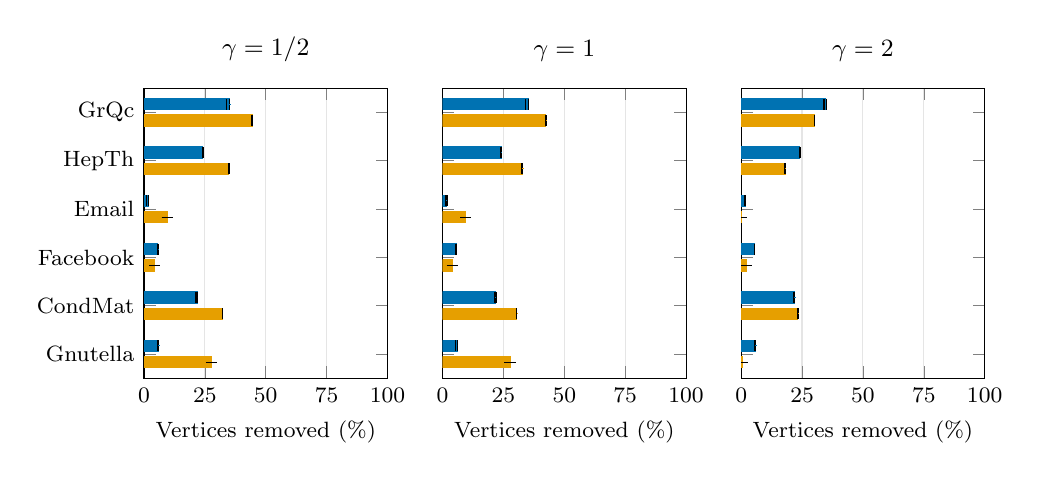
\begin{tikzpicture}
\begin{groupplot}[group style={group size=3 by 1,horizontal sep=7mm},scale only axis,width=.255\textwidth,height=1.45in,xmin=0,xmax=100,ymin=-.5,ymax=5.5,xtick={0,25,50,75,100},ytick={0,1,2,3,4,5},y dir=reverse,xlabel={Vertices removed (\%)},tick label style={font=\footnotesize},label style={font=\footnotesize},title style={font=\small},xmajorgrids,grid style={gray!20}]
\nextgroupplot[title={$\gamma=1/2$},yticklabels={GrQc,HepTh,Email,Facebook,CondMat,Gnutella}]
\addplot[xbar,bar width=4pt,fill=proposalblue,draw=proposalblue,error bars/.cd,x dir=both,x explicit] table[row sep=\\,x=x,y=y,x error minus=lo,x error plus=hi]{x y lo hi\\
35.1201831 -0.17 1.08737123 0.133536818\\
24.1267591 0.83 0.202490635 0.242988762\\
1.69154229 1.83 0.497512438 0.0995024876\\
5.64496162 2.83 0.0495172072 0.0990344145\\
21.9124195 3.83 0.540353607 0.0259369732\\
6.04665926 4.83 0.63481987 0.0158704967\\
};
\addplot[xbar,bar width=4pt,fill=referenceorange,draw=referenceorange,error bars/.cd,x dir=both,x explicit] table[row sep=\\,x=x,y=y,x error minus=lo,x error plus=hi]{x y lo hi\\
44.4105303 0.17 0.0763067531 0.228920259\\
34.8385137 1.17 0.273362357 0.151867976\\
9.55223881 2.17 0 0\\
4.33275563 3.17 0 0\\
32.0840358 4.17 0.00432282886 0.0432282886\\
27.6940168 5.17 0 0\\
};
\nextgroupplot[title={$\gamma=1$},yticklabels=\empty]
\addplot[xbar,bar width=4pt,fill=proposalblue,draw=proposalblue,error bars/.cd,x dir=both,x explicit] table[row sep=\\,x=x,y=y,x error minus=lo,x error plus=hi]{x y lo hi\\
35.1201831 -0.17 1.08737123 0.133536818\\
24.1267591 0.83 0.202490635 0.242988762\\
1.69154229 1.83 0.497512438 0.0995024876\\
5.52116861 2.83 0.0247586036 0.222827433\\
21.9124195 3.83 0.540353607 0.0259369732\\
6.04665926 4.83 0.63481987 0.0158704967\\
};
\addplot[xbar,bar width=4pt,fill=referenceorange,draw=referenceorange,error bars/.cd,x dir=both,x explicit] table[row sep=\\,x=x,y=y,x error minus=lo,x error plus=hi]{x y lo hi\\
42.3884014 0.17 0.11446013 0.0953834414\\
32.8541055 1.17 0.303735952 0.101245317\\
9.55223881 2.17 0 0\\
4.06041099 3.17 0 0\\
30.4500065 4.17 0.0172913154 0.060519604\\
27.6940168 5.17 0 0\\
};
\nextgroupplot[title={$\gamma=2$},yticklabels=\empty]
\addplot[xbar,bar width=4pt,fill=proposalblue,draw=proposalblue,error bars/.cd,x dir=both,x explicit] table[row sep=\\,x=x,y=y,x error minus=lo,x error plus=hi]{x y lo hi\\
34.6623426 -0.17 0.629530713 0.343380389\\
24.1267591 0.83 0.202490635 0.242988762\\
1.69154229 1.83 0.497512438 0.0995024876\\
5.4716514 2.83 0.123793018 0.173310225\\
21.9124195 3.83 0.540353607 0.0259369732\\
6.04665926 4.83 0.63481987 0.0158704967\\
};
\addplot[xbar,bar width=4pt,fill=referenceorange,draw=referenceorange,error bars/.cd,x dir=both,x explicit] table[row sep=\\,x=x,y=y,x error minus=lo,x error plus=hi]{x y lo hi\\
30.0457841 0.17 0.0572300649 0.190766883\\
18.011542 1.17 0.0607471904 0.0303735952\\
0.0995024876 2.17 0 0\\
2.20351572 3.17 0 0\\
23.2914019 4.17 0.0216141443 0.0345826309\\
0.476114902 5.17 0 0\\
};
\end{groupplot}
\end{tikzpicture}
\caption{Public coverage. Blue: degree-weighted certificate; orange: recursive named criteria on the same bank. Bars show median removed fractions over three discovery seeds; whiskers show the observed range. All vertices remain in the denominator.}\label{fig:coverage}
\end{figure*}
% END GENERATED COVERAGE FIGURE

% BEGIN GENERATED UTILITY FIGURE
\begin{figure*}[t]
\centering
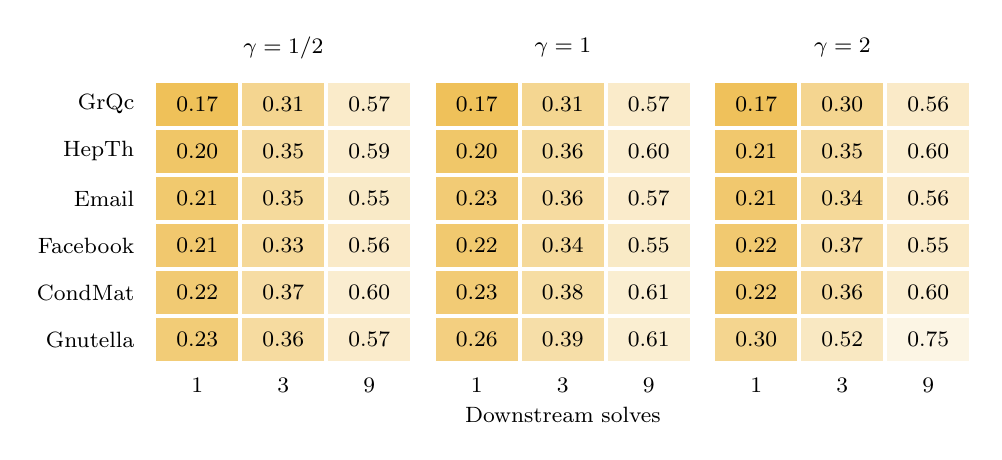
\begin{tikzpicture}[x=.43in,y=.235in,every node/.style={font=\footnotesize}]
\node[anchor=east] at (-.12,5.5) {GrQc};
\node[anchor=east] at (-.12,4.5) {HepTh};
\node[anchor=east] at (-.12,3.5) {Email};
\node[anchor=east] at (-.12,2.5) {Facebook};
\node[anchor=east] at (-.12,1.5) {CondMat};
\node[anchor=east] at (-.12,0.5) {Gnutella};
\node at (1.5,6.7) {$\gamma=1/2$};
\node at (0.5,-.48) {1};
\node at (1.5,-.48) {3};
\node at (2.5,-.48) {9};
\filldraw[fill=referenceorange!65.000!white,draw=white,line width=1.5pt] (0.0,5) rectangle (1.0,6);
\node at (0.5,5.5) {0.17};
\filldraw[fill=referenceorange!43.548!white,draw=white,line width=1.5pt] (1.0,5) rectangle (2.0,6);
\node at (1.5,5.5) {0.31};
\filldraw[fill=referenceorange!20.750!white,draw=white,line width=1.5pt] (2.0,5) rectangle (3.0,6);
\node at (2.5,5.5) {0.57};
\filldraw[fill=referenceorange!59.547!white,draw=white,line width=1.5pt] (0.0,4) rectangle (1.0,5);
\node at (0.5,4.5) {0.20};
\filldraw[fill=referenceorange!38.230!white,draw=white,line width=1.5pt] (1.0,4) rectangle (2.0,5);
\node at (1.5,4.5) {0.35};
\filldraw[fill=referenceorange!19.449!white,draw=white,line width=1.5pt] (2.0,4) rectangle (3.0,5);
\node at (2.5,4.5) {0.59};
\filldraw[fill=referenceorange!56.698!white,draw=white,line width=1.5pt] (0.0,3) rectangle (1.0,4);
\node at (0.5,3.5) {0.21};
\filldraw[fill=referenceorange!38.826!white,draw=white,line width=1.5pt] (1.0,3) rectangle (2.0,4);
\node at (1.5,3.5) {0.35};
\filldraw[fill=referenceorange!22.044!white,draw=white,line width=1.5pt] (2.0,3) rectangle (3.0,4);
\node at (2.5,3.5) {0.55};
\filldraw[fill=referenceorange!57.043!white,draw=white,line width=1.5pt] (0.0,2) rectangle (1.0,3);
\node at (0.5,2.5) {0.21};
\filldraw[fill=referenceorange!40.245!white,draw=white,line width=1.5pt] (1.0,2) rectangle (2.0,3);
\node at (1.5,2.5) {0.33};
\filldraw[fill=referenceorange!21.569!white,draw=white,line width=1.5pt] (2.0,2) rectangle (3.0,3);
\node at (2.5,2.5) {0.56};
\filldraw[fill=referenceorange!54.850!white,draw=white,line width=1.5pt] (0.0,1) rectangle (1.0,2);
\node at (0.5,1.5) {0.22};
\filldraw[fill=referenceorange!36.068!white,draw=white,line width=1.5pt] (1.0,1) rectangle (2.0,2);
\node at (1.5,1.5) {0.37};
\filldraw[fill=referenceorange!18.582!white,draw=white,line width=1.5pt] (2.0,1) rectangle (3.0,2);
\node at (2.5,1.5) {0.60};
\filldraw[fill=referenceorange!53.479!white,draw=white,line width=1.5pt] (0.0,0) rectangle (1.0,1);
\node at (0.5,0.5) {0.23};
\filldraw[fill=referenceorange!37.375!white,draw=white,line width=1.5pt] (1.0,0) rectangle (2.0,1);
\node at (1.5,0.5) {0.36};
\filldraw[fill=referenceorange!20.363!white,draw=white,line width=1.5pt] (2.0,0) rectangle (3.0,1);
\node at (2.5,0.5) {0.57};
\node at (4.75,6.7) {$\gamma=1$};
\node at (3.75,-.48) {1};
\node at (4.75,-.48) {3};
\node at (5.75,-.48) {9};
\filldraw[fill=referenceorange!64.576!white,draw=white,line width=1.5pt] (3.25,5) rectangle (4.25,6);
\node at (3.75,5.5) {0.17};
\filldraw[fill=referenceorange!42.994!white,draw=white,line width=1.5pt] (4.25,5) rectangle (5.25,6);
\node at (4.75,5.5) {0.31};
\filldraw[fill=referenceorange!20.766!white,draw=white,line width=1.5pt] (5.25,5) rectangle (6.25,6);
\node at (5.75,5.5) {0.57};
\filldraw[fill=referenceorange!58.833!white,draw=white,line width=1.5pt] (3.25,4) rectangle (4.25,5);
\node at (3.75,4.5) {0.20};
\filldraw[fill=referenceorange!37.991!white,draw=white,line width=1.5pt] (4.25,4) rectangle (5.25,5);
\node at (4.75,4.5) {0.36};
\filldraw[fill=referenceorange!18.780!white,draw=white,line width=1.5pt] (5.25,4) rectangle (6.25,5);
\node at (5.75,4.5) {0.60};
\filldraw[fill=referenceorange!53.985!white,draw=white,line width=1.5pt] (3.25,3) rectangle (4.25,4);
\node at (3.75,3.5) {0.23};
\filldraw[fill=referenceorange!37.425!white,draw=white,line width=1.5pt] (4.25,3) rectangle (5.25,4);
\node at (4.75,3.5) {0.36};
\filldraw[fill=referenceorange!20.377!white,draw=white,line width=1.5pt] (5.25,3) rectangle (6.25,4);
\node at (5.75,3.5) {0.57};
\filldraw[fill=referenceorange!56.453!white,draw=white,line width=1.5pt] (3.25,2) rectangle (4.25,3);
\node at (3.75,2.5) {0.22};
\filldraw[fill=referenceorange!39.495!white,draw=white,line width=1.5pt] (4.25,2) rectangle (5.25,3);
\node at (4.75,2.5) {0.34};
\filldraw[fill=referenceorange!22.224!white,draw=white,line width=1.5pt] (5.25,2) rectangle (6.25,3);
\node at (5.75,2.5) {0.55};
\filldraw[fill=referenceorange!53.932!white,draw=white,line width=1.5pt] (3.25,1) rectangle (4.25,2);
\node at (3.75,1.5) {0.23};
\filldraw[fill=referenceorange!35.911!white,draw=white,line width=1.5pt] (4.25,1) rectangle (5.25,2);
\node at (4.75,1.5) {0.38};
\filldraw[fill=referenceorange!18.101!white,draw=white,line width=1.5pt] (5.25,1) rectangle (6.25,2);
\node at (5.75,1.5) {0.61};
\filldraw[fill=referenceorange!49.984!white,draw=white,line width=1.5pt] (3.25,0) rectangle (4.25,1);
\node at (3.75,0.5) {0.26};
\filldraw[fill=referenceorange!34.164!white,draw=white,line width=1.5pt] (4.25,0) rectangle (5.25,1);
\node at (4.75,0.5) {0.39};
\filldraw[fill=referenceorange!18.029!white,draw=white,line width=1.5pt] (5.25,0) rectangle (6.25,1);
\node at (5.75,0.5) {0.61};
\node at (8.0,6.7) {$\gamma=2$};
\node at (7.0,-.48) {1};
\node at (8.0,-.48) {3};
\node at (9.0,-.48) {9};
\filldraw[fill=referenceorange!64.346!white,draw=white,line width=1.5pt] (6.5,5) rectangle (7.5,6);
\node at (7.0,5.5) {0.17};
\filldraw[fill=referenceorange!43.634!white,draw=white,line width=1.5pt] (7.5,5) rectangle (8.5,6);
\node at (8.0,5.5) {0.30};
\filldraw[fill=referenceorange!21.387!white,draw=white,line width=1.5pt] (8.5,5) rectangle (9.5,6);
\node at (9.0,5.5) {0.56};
\filldraw[fill=referenceorange!57.102!white,draw=white,line width=1.5pt] (6.5,4) rectangle (7.5,5);
\node at (7.0,4.5) {0.21};
\filldraw[fill=referenceorange!38.057!white,draw=white,line width=1.5pt] (7.5,4) rectangle (8.5,5);
\node at (8.0,4.5) {0.35};
\filldraw[fill=referenceorange!18.934!white,draw=white,line width=1.5pt] (8.5,4) rectangle (9.5,5);
\node at (9.0,4.5) {0.60};
\filldraw[fill=referenceorange!56.941!white,draw=white,line width=1.5pt] (6.5,3) rectangle (7.5,4);
\node at (7.0,3.5) {0.21};
\filldraw[fill=referenceorange!39.844!white,draw=white,line width=1.5pt] (7.5,3) rectangle (8.5,4);
\node at (8.0,3.5) {0.34};
\filldraw[fill=referenceorange!21.508!white,draw=white,line width=1.5pt] (8.5,3) rectangle (9.5,4);
\node at (9.0,3.5) {0.56};
\filldraw[fill=referenceorange!55.898!white,draw=white,line width=1.5pt] (6.5,2) rectangle (7.5,3);
\node at (7.0,2.5) {0.22};
\filldraw[fill=referenceorange!36.568!white,draw=white,line width=1.5pt] (7.5,2) rectangle (8.5,3);
\node at (8.0,2.5) {0.37};
\filldraw[fill=referenceorange!21.861!white,draw=white,line width=1.5pt] (8.5,2) rectangle (9.5,3);
\node at (9.0,2.5) {0.55};
\filldraw[fill=referenceorange!54.940!white,draw=white,line width=1.5pt] (6.5,1) rectangle (7.5,2);
\node at (7.0,1.5) {0.22};
\filldraw[fill=referenceorange!37.144!white,draw=white,line width=1.5pt] (7.5,1) rectangle (8.5,2);
\node at (8.0,1.5) {0.36};
\filldraw[fill=referenceorange!18.926!white,draw=white,line width=1.5pt] (8.5,1) rectangle (9.5,2);
\node at (9.0,1.5) {0.60};
\filldraw[fill=referenceorange!44.017!white,draw=white,line width=1.5pt] (6.5,0) rectangle (7.5,1);
\node at (7.0,0.5) {0.30};
\filldraw[fill=referenceorange!24.043!white,draw=white,line width=1.5pt] (7.5,0) rectangle (8.5,1);
\node at (8.0,0.5) {0.52};
\filldraw[fill=referenceorange!10.632!white,draw=white,line width=1.5pt] (8.5,0) rectangle (9.5,1);
\node at (9.0,0.5) {0.75};
\node at (4.75,-1.1) {Downstream solves};
\end{tikzpicture}
\caption{Cost recovery: median matched warm unreduced-to-reduced total-time ratio over three discovery seeds. Values above 1 recover the full reduction cost; values below 1 retain the overhead. Blue denotes recovery and orange denotes overhead; color intensity uses a common symmetric logarithmic scale about 1.}\label{fig:utility}
\end{figure*}
% END GENERATED UTILITY FIGURE

% BEGIN GENERATED coverage-details TABLE
\begin{table*}[t]
\caption{Complete v1 public coverage. Entries are median [minimum,maximum] over three discovery seeds. D and R denote the degree certificate and the specified recursive criteria. Join ranks compare the structural partitions; they are not an executed safe hybrid pipeline.}\label{tab:coverage-details}
\centering\small
\begin{tabular}{lcrrrr}\toprule
Graph & $\gamma$ & D removed (\%) & R removed (\%) & D beyond R & R beyond D\\\midrule
GrQc & $1/2$ & 35.1 [34.0,35.3] & 44.4 [44.3,44.6] & 216 [174,218] & 715 [694,718]\\
GrQc & $1$ & 35.1 [34.0,35.3] & 42.4 [42.3,42.5] & 250 [209,257] & 643 [618,647]\\
GrQc & $2$ & 34.7 [34.0,35.0] & 30.0 [30.0,30.2] & 463 [419,476] & 220 [213,221]\\
HepTh & $1/2$ & 24.1 [23.9,24.4] & 34.8 [34.6,35.0] & 324 [322,347] & 1397 [1356,1398]\\
HepTh & $1$ & 24.1 [23.9,24.4] & 32.9 [32.6,33.0] & 366 [353,380] & 1232 [1191,1238]\\
HepTh & $2$ & 24.1 [23.9,24.4] & 18.0 [18.0,18.0] & 874 [868,893] & 268 [264,284]\\
Email & $1/2$ & 1.7 [1.2,1.8] & 9.6 [9.6,9.6] & 0 [0,1] & 79 [79,84]\\
Email & $1$ & 1.7 [1.2,1.8] & 9.6 [9.6,9.6] & 0 [0,1] & 79 [79,84]\\
Email & $2$ & 1.7 [1.2,1.8] & 0.1 [0.1,0.1] & 17 [12,18] & 1 [1,1]\\
Facebook & $1/2$ & 5.6 [5.6,5.7] & 4.3 [4.3,4.3] & 145 [143,149] & 92 [88,96]\\
Facebook & $1$ & 5.5 [5.5,5.7] & 4.1 [4.1,4.1] & 147 [142,148] & 83 [79,90]\\
Facebook & $2$ & 5.5 [5.3,5.6] & 2.2 [2.2,2.2] & 153 [149,159] & 21 [20,22]\\
CondMat & $1/2$ & 21.9 [21.4,21.9] & 32.1 [32.1,32.1] & 733 [697,757] & 3103 [3096,3175]\\
CondMat & $1$ & 21.9 [21.4,21.9] & 30.5 [30.4,30.5] & 796 [765,825] & 2790 [2785,2865]\\
CondMat & $2$ & 21.9 [21.4,21.9] & 23.3 [23.3,23.3] & 1376 [1309,1393] & 1703 [1701,1753]\\
Gnutella & $1/2$ & 6.0 [5.4,6.1] & 27.7 [27.7,27.7] & 0 [0,0] & 1364 [1363,1404]\\
Gnutella & $1$ & 6.0 [5.4,6.1] & 27.7 [27.7,27.7] & 0 [0,0] & 1364 [1363,1404]\\
Gnutella & $2$ & 6.0 [5.4,6.1] & 0.5 [0.5,0.5] & 355 [316,356] & 4 [4,5]\\
\bottomrule\end{tabular}
\end{table*}
% END GENERATED coverage-details TABLE

% BEGIN GENERATED cost-cap-details TABLE
\begin{table*}[t]
\caption{Complete v1 checking and preprocessing cost, cap exclusions, and largest-component coverage, as median [minimum,maximum] over three discovery seeds. Component coverage retains the original full-graph objective and volume. Preprocessing includes the declared original representation, discovery, refinement, checker, quotient and solver-interface work.}\label{tab:cost-cap-details}
\centering\small
\begin{tabular}{lcrrrr}\toprule
Graph & $\gamma$ & Checker (s) & Preprocessing (s) & Cap exclusions & LCC removed (\%)\\\midrule
GrQc & $1/2$ & 0.520 [0.507,0.538] & 1.199 [1.187,1.213] & 68 [64,70] & 26.7 [25.3,26.9]\\
GrQc & $1$ & 0.518 [0.502,0.557] & 1.199 [1.194,1.245] & 68 [64,70] & 26.7 [25.3,26.9]\\
GrQc & $2$ & 0.513 [0.509,0.516] & 1.199 [1.193,1.209] & 68 [64,70] & 26.1 [25.3,26.6]\\
HepTh & $1/2$ & 0.899 [0.874,0.957] & 2.488 [2.479,2.610] & 174 [171,176] & 18.2 [18.0,18.5]\\
HepTh & $1$ & 0.956 [0.910,0.988] & 2.553 [2.505,2.634] & 174 [171,176] & 18.2 [18.0,18.5]\\
HepTh & $2$ & 0.875 [0.874,0.954] & 2.528 [2.489,2.575] & 174 [171,176] & 18.2 [18.0,18.5]\\
Email & $1/2$ & 0.148 [0.127,0.157] & 0.430 [0.407,0.449] & 16 [14,18] & 1.7 [1.2,1.8]\\
Email & $1$ & 0.144 [0.128,0.145] & 0.437 [0.410,0.444] & 16 [14,18] & 1.7 [1.2,1.8]\\
Email & $2$ & 0.153 [0.129,0.204] & 0.437 [0.410,0.504] & 16 [14,18] & 1.7 [1.2,1.8]\\
Facebook & $1/2$ & 0.648 [0.640,0.707] & 2.044 [2.031,2.280] & 85 [84,86] & 5.6 [5.6,5.7]\\
Facebook & $1$ & 0.695 [0.640,0.728] & 2.147 [2.075,2.214] & 85 [84,86] & 5.5 [5.5,5.7]\\
Facebook & $2$ & 0.689 [0.644,0.721] & 2.140 [2.079,2.261] & 85 [84,86] & 5.5 [5.3,5.6]\\
CondMat & $1/2$ & 2.266 [2.242,2.447] & 6.886 [6.774,7.065] & 494 [485,509] & 18.1 [17.5,18.1]\\
CondMat & $1$ & 2.248 [2.241,2.269] & 6.855 [6.744,6.928] & 494 [485,509] & 18.1 [17.5,18.1]\\
CondMat & $2$ & 2.275 [2.259,2.293] & 6.892 [6.848,6.923] & 494 [485,509] & 18.1 [17.5,18.1]\\
Gnutella & $1/2$ & 0.510 [0.508,0.530] & 1.866 [1.832,1.877] & 155 [144,158] & 6.0 [5.4,6.0]\\
Gnutella & $1$ & 0.516 [0.499,0.519] & 1.872 [1.828,1.877] & 155 [144,158] & 6.0 [5.4,6.0]\\
Gnutella & $2$ & 0.528 [0.507,0.575] & 1.869 [1.866,1.903] & 155 [144,158] & 6.0 [5.4,6.0]\\
\bottomrule\end{tabular}
\end{table*}
% END GENERATED cost-cap-details TABLE

% BEGIN GENERATED mechanism-details TABLE
\begin{table*}[t]
\caption{Every controlled supplied-block family and resolution. Counts are certified blocks over denominator N; U denotes unavailable comparisons, not mathematical rejection. AUTO is the production median checker; Exact is its forced exact counterpart. Zero and Full pair are independent rational reference conditions. The uniform reference retains its frozen graph-size guard. Private leaves are exploratory stress controls.}\label{tab:mechanism-details}
\centering\small
\begin{tabular}{lcrrrrrr}\toprule
Family & $\gamma$ & N & AUTO & Exact & Zero & Full pair & Uniform\\\midrule
Matched cliques & $1/2$ & 14 & 14 & 14 & 14 & 14 & 14\\
Matched cliques & $1$ & 14 & 10 & 12 & 12 & 12 & 12\\
Matched cliques & $2$ & 14 & 0 & 0 & 0 & 0 & 0\\
Common hubs & $1/2$ & 2 & 2 & 2 & 2 & 2 & 2\\
Common hubs & $1$ & 2 & 2 & 2 & 1 & 2 & 2\\
Common hubs & $2$ & 2 & 0 & 0 & 0 & 0 & 0\\
Weighted blocks & $1/2$ & 9 & 9 & 9 & 9 & 9 & 7\\
Weighted blocks & $1$ & 9 & 9 & 9 & 9 & 9 & 3\\
Weighted blocks & $2$ & 9 & 6 & 6 & 6 & 6 & 0\\
Noisy blocks & $1/2$ & 192 & 110 & 110 & 110 & 116 & 0 (192 U)\\
Noisy blocks & $1$ & 192 & 88 & 88 & 88 & 90 & 0 (192 U)\\
Noisy blocks & $2$ & 192 & 50 & 50 & 50 & 51 & 0 (192 U)\\
Exterior profiles & $1/2$ & 6 & 6 & 6 & 6 & 6 & 2 (4 U)\\
Exterior profiles & $1$ & 6 & 6 & 6 & 4 & 6 & 2 (4 U)\\
Exterior profiles & $2$ & 6 & 4 & 4 & 3 & 4 & 0 (4 U)\\
Uniform advantage & $1/8$ & 1 & 0 & 0 & 0 & 0 & 1\\
Private leaves & $1$ & 3 & 0 & 0 & 0 & 0 & 0\\
\bottomrule\end{tabular}
\end{table*}
% END GENERATED mechanism-details TABLE

\end{document}
